% ---------------------------------------------------------------------
%                      DOCUMENTO DE EJEMPLO
%                    QUE UTILIZA LA PLANTILLA
%                      DE LA EDITORIAL DE LA
%                UNIVERSITAT POLITÈCNICA DE VALÈNCIA
% ---------------------------------------------------------------------

\documentclass[tesi, crop, rm, english]{editorialupv}
\usepackage{amsmath}
\DeclareMathOperator*{\argmin}{arg\,min}
% Opciones de la clase 'editorialupv'
%
% llibre      - Libro docente
% ebookpdf    - Libro en formato PDF para e-Readers
% tesi        - Formato de tesis
% a4          - Formato A4
% rm          - Tipo de letra roman
% sf          - Tipo de letra sanserif
% crop        - Marcas de corte (cruz) 17x24 cm (+3 mm por los cuatro lados) centrada en una A4 
% nocrop      - Sin marcas de corte, respeta el tamaño 17x24 cm 
% nomathskip  - No se modifican las distancias de las ecuaciones 
%
% castellano  - La publicación está escrita en castellano
% valencia    - La publicació està escrita en valencià
% english     - La publicación está escrita en inglés

% ---------------------------------------------------------------------
% Configuraciones presonalizadas 

% ---------------------------------------------------------------------
% ---------------------------------------------------------------------
% Configuración general

\usepackage[utf8]{inputenc}
\usepackage[T1]{fontenc}

\ifEPUB
	% Soluciona error "Undefined control sequence \blx@shorthands" cuando backend=biber 
	% Con bibtex no da este error
	\makeatletter
	\def\blx@shorthands{} 
	\makeatother 

	\ifcastellano\usepackage[spanish,es-tabla,es-sloppy]{babel}\fi
	\ifvalencia\usepackage[catalan]{babel}\fi
	\ifenglish\usepackage[english]{babel}\fi
	\newcommand{\sen}{\on{sen}}
	\date{}
\else
	\ifcastellano\usepackage[spanish,es-tabla]{babel}\fi
	\ifvalencia\usepackage[catalan]{babel}\fi
	\ifenglish\usepackage[english]{babel}\usepackage{csquotes}\fi
	\newcommand{\sen}{\on{sen}}	
\fi

\usepackage{xcolor}
\usepackage{array,booktabs}
\usepackage{tabularx,longtable,multicol}
\usepackage{amssymb}

%\ifenglish
%	\raggedright % No justifica, i no divide las palabras con guiones
%\fi

% ---------------------------------------------------------------------
% ---------------------------------------------------------------------
% Bibliografía

\usepackage[
	url = false,
	style = authoryear,
	hyperref = true,
	backref = true,
	backend = biber, % Otra opción es 'backend = bibtex'
	]{biblatex}

% ---------------------------------------------------------------------
% ---------------------------------------------------------------------
% Documento electrónico

\usepackage{makeidx}
\makeindex

\ifEBOOKPDF
	\colorlet{colorEnlace}{red!75!black} 
\else 
	\colorlet{colorEnlace}{black} 
\fi

\usepackage[
	{colorlinks},
	{linkcolor=colorEnlace},
	{citecolor=colorEnlace},
	{urlcolor=colorEnlace},
	{bookmarksnumbered},
	{breaklinks},
	]{hyperref}

% ---------------------------------------------------------------------
% ---------------------------------------------------------------------
% Expresión de unidades según el Sistema Internacional, monedas

\usepackage{eurosym}
\usepackage{siunitx}

\ifenglish
	\sisetup{output-decimal-marker={.}}
\else
	\sisetup{output-decimal-marker={,}}
\fi

\DeclareSIUnit[number-unit-product = {\;}] \EURO{\geneuro}

% ---------------------------------------------------------------------
% ---------------------------------------------------------------------
% Comandos y entornos personalizados

\ifEPUB
	\renewcommand{\includegraphics}[2][]{\Picture[#2]{./figuras/#2.png width="500px"}}
\fi

% ---------------------------------------------------------------------
% ---------------------------------------------------------------------
% Por compatibilidad con versiones anteriores de la plantilla

\ifEPUB
	\newcommand{\incluyeGrafico}[2][]{\Picture[#2]{./figuras/#2.png width="500px"}} % Por compatibilidad
\else		
	\newcommand{\incluyeGrafico}[2][]{\includegraphics[#1]{#2}} % Por compatibilidad
\fi

% ---------------------------------------------------------------------

\newcommand{\ingles}[1]{\textit{#1}}

% ------------------------------------------------------------------------

\usepackage{xspace}

\newcommand{\angles}[1]{\textit{#1}\/}
\newcommand{\miUrl}[1]{{\small%
	%\texttt%
	{\underline{#1}}}}

\newcommand{\matlabr}{{\sc Matlab}$^\circledR$\xspace}
\newcommand{\simulinkr}{\textit{Simulink}$^\circledR$\xspace}
\newcommand{\matlab}{{\textsc{Matlab}}\xspace}
\newcommand{\simulink}{\textit{Simulink}\xspace}

\newcommand{\scr}{\textit{script\/}\xspace}
\newcommand{\scrs}{\textit{scripts\/}\xspace}

% ------------------------------------------------------------------------

\definecolor{griset}{rgb}{.925, .925, .925}

\ifEPUB

	\newenvironment{parrafoDestacado}
		{
		\HCode{<div class="parrafoDestacado">}
		}
		{
		\HCode{</div>}	
		}

\else

	\newsavebox{\mybox}
	\newenvironment{parrafoDestacado}
		{%
		\fboxsep = 2ex
		\fboxrule = .4pt
	  	\begin{lrbox}{\mybox}%
	  	\begin{minipage}{.85\textwidth-2\fboxsep}\itshape\parskip=2ex
		}
		{%
		\end{minipage}
	  	\end{lrbox}%
		\begin{flushright}
			\colorbox{griset}{\usebox{\mybox}}%
	  		%\fcolorbox{black}{griset}{\usebox{\mybox}}%
		\end{flushright}
		}
		
%	\newenvironment{parrafoDestacado} % Si no nos gusta el sombreado
%		{
%		\vspace{0ex}
%		\begin{quote}\noindent
%		\itshape
%		\samepage
%		\parskip=2ex
%		%\color{NavyBlue}
%		}
%		{
%		\end{quote}
%		}

\fi

% ------------------------------------------------------------------------
% Resumen del capítulo

\ifEPUB

	\newenvironment{Resumen}
		{
		\HCode{<div class="Resumen">}
		}
		{
		\HCode{</div>}	
		}

\else

	\newsavebox{\myboxb}
	\newenvironment{Resumen}
		{%
		\vspace*{-2.0cm}
		\fboxsep = 0pt
		\fboxrule = 0pt
	  	\begin{lrbox}{\myboxb}%
	  	\begin{minipage}{.85\textwidth}\itshape\parskip=2ex\parindent=2em
		}
		{%
		\end{minipage}
	  	\end{lrbox}%
		\begin{flushright}
			\usebox{\myboxb}%
		\end{flushright}
		\vspace{0.5cm}
		}

\fi

% ---------------------------------------------------------------------
% ---------------------------------------------------------------------
% Símbolos matemáticos

\newcommand{\on}{\operatorname}

% ---------------------------------------------------------------------
% ---------------------------------------------------------------------
% Teoremas y ejemplos

\ifcastellano
	\newtheorem{teorema}{\upshape\bfseries Teorema}[section]
	\newtheorem{lema}{\mdseries\scshape Lema}[section]
	\newtheorem{proposicion}{\upshape\bfseries Proposición}[section]
	\newtheorem{ejemplo}{\bfseries\scshape Ejemplo}[section]
\fi

\ifvalencia % Es mantenen els mateixos noms per compatibilitat, però l'autor els pot personalitzar
	\newtheorem{teorema}{\upshape\bfseries Teorema}[section]
	\newtheorem{lema}{\mdseries\scshape Lema}[section]
	\newtheorem{proposicion}{\upshape\bfseries Proposició}[section]
	\newtheorem{ejemplo}{\bfseries\scshape Exemple}[section]
\fi

\ifenglish
	\newtheorem{teorema}{\upshape\bfseries Theorem}[section]
	\newtheorem{lema}{\mdseries\scshape Lemma}[section]
	\newtheorem{proposicion}{\upshape\bfseries Proposition}[section]
	\newtheorem{ejemplo}{\bfseries\scshape Example}[section]
\fi


% ---------------------------------------------------------------------
% Obsoleto

% En esta versión de la plantilla no es necesario utilizar el comando \ parBlanca 
% Pero lo mantenemos por compatibilidad

\newcommand
	{\parBlanca}
	{\clearpage{\thispagestyle{empty}\cleardoublepage}}


% ---------------------------------------------------------------------



\bibliography{referencias}

% ---------------------------------------------------------------------
% Las carpetas para los gráficos

\graphicspath{
	{../figuras/}
	{../logos/}
	{./figuras/}
	{./logos/}
	}

% ---------------------------------------------------------------------

\title{
	Use of multivariate statistical methods for the analysis of metabolomic data\\[3ex]
	\mdseries\large	October 2018
	}


% ---------------------------------------------------------------------
% Para una tesis se recomienda utilizar esta estructura para el autor y directores de tesis

\author{
	\parbox{\textwidth}{\centering%
		\begin{tabular}{l@{\hspace{.75em}}l}
			Author: 		& David Hervás Marín\\[4ex]
			Director: 	& José Manuel Prats Montalbán\\[.5ex]
						& Agustín Lahoz Rodríguez
		\end{tabular}
		}
	}


% ---------------------------------------------------------------------
% ---------------------------------------------------------------------
% ---------------------------------------------------------------------

\begin{document}

% ---------------------------------------------------------------------
% Referencias cruzadas personalizadas y texto automático de LaTeX

\ifcastellano % Las definiciones predefinidas empiezan con mayúscula
	\renewcommand{\itemautorefname}{punto}
	\renewcommand{\sectionautorefname}{sección}
	\renewcommand{\subsectionautorefname}{subsección}
	\renewcommand{\subsubsectionautorefname}{subsección}
	\renewcommand{\figureautorefname}{figura}
	\renewcommand{\tableautorefname}{tabla}
	
	\renewcommand{\indexname}{Índice alfabético}
	\renewcommand{\bibname}{Bibliografía}
	\renewcommand{\contentsname}{Índice general}
	\renewcommand{\abstractname}{Resumen}	
\fi

\ifvalencia % És molt important fer aquestes definicions, si no, apareixeran en anglès
	\renewcommand{\itemautorefname}{punt}
	\renewcommand{\sectionautorefname}{secció}
	\renewcommand{\subsectionautorefname}{subsecció}
	\renewcommand{\subsubsectionautorefname}{subsecció}
	\renewcommand{\figureautorefname}{figura}
	\renewcommand{\tableautorefname}{taula}

	\renewcommand{\indexname}{Índex alfabètic}
	\renewcommand{\bibname}{Bibliografia}
	\renewcommand{\contentsname}{Índex}
	\renewcommand{\abstractname}{Resum}	
\fi

% -------------------------------------------------------

\frontmatter

% -------------------------------------------------------
% Página de título

\maketitle	

% -------------------------------------------------------
% Resumen, prólogo o prefacio
\addcontentsline{toc}{chapter}{Acknowledgments}
\chapter*{Acknowledgments}

% ---------------------------------------------------------------------
% ---------------------------------------------------------------------
% ---------------------------------------------------------------------

Writing a thesis always involves a lot of working, fighting against adversity and enduring numerous obstacles. This one is no exception, and it wouldn’t have been finished without the help of my two directors José Manuel Prats Montalbán and Agustín Lahoz Rodríguez. 

I want to thank also the help and insights given by Alberto Ferrer Riquelme, who has greatly contributed with his knowledge to the contents of this work.

Special thanks to Victoria Fornés Ferrer for her help with the valencian version of the abstract and for being such a great colleage.

Finally, some lines to my parents Ana and Tomás, my brother Raúl, my wife Lucía and my precious daughter Laura. Thank you for your support, for your patience and your love. This thesis is dedicated to you all.


\cleardoublepage
\phantomsection
\addcontentsline{toc}{chapter}{\abstractname}


% ---------------------------------------------------------------------
% ---------------------------------------------------------------------
% ---------------------------------------------------------------------

\chapter*{Resumen}

% ---------------------------------------------------------------------
% ---------------------------------------------------------------------
% ---------------------------------------------------------------------

En las últimas décadas los avances tecnológicos han tenido como consecuencia la generación de una creciente cantidad de datos en el campo de la biología y la biomedicina. A día de hoy, las así llamadas tecnologías “ómicas”, como la genómica, epigenómica, transcriptómica o metabolómica entre otras, producen bases de datos con cientos, miles o incluso millones de variables. 

El análisis de datos ómicos presenta una serie de complejidades tanto metodológicas como computacionales que han llevado a una revolución en el desarrollo de nuevos métodos estadísticos específicamente diseñados para tratar con este tipo de datos. 

A estas complejidades metodológicas hay que añadir que, en la mayor parte de los casos, las restricciones logísticas y/o económicas de los proyectos de investigación suelen conllevar que los tamaños muestrales en estas bases de datos con tantas variables sean muy bajos, lo cual no hace sino empeorar las dificultades de análisis, ya que se tienen muchísimas más variables que observaciones.

Entre las técnicas desarrolladas para tratar con este tipo de datos podemos encontrar algunas basadas en la penalización de los coeficientes, como lasso o elastic net, otras basadas en técnicas de proyección sobre estructuras latentes como PCA o PLS y otras basadas en árboles o combinaciones de árboles como random forest.

Todas estas técnicas funcionan muy bien sobre distritos datos ómicos presentados en forma de matriz (IxJ), sin embargo, en ocasiones los datos ómicos pueden estar expandidos, por ejemplo, al tomar medidas repetidas en el tiempo sobre los mismos individuos, encontrándonos con estructuras de datos que ya no son matrices, sino arrays tridimensionales o three-way (IxJxK). En estos casos, la mayoría de las técnicas citadas pierden toda o buena parte de su aplicabilidad, quedando muy pocas opciones viables para el análisis de este tipo de estructuras de datos.

Una de las técnicas que sí es útil para el análisis de estructuras three-way es $N$-PLS, que permite ajustar modelos predictivos razonablemente precisos, así como interpretarlos mediante distintos gráficos.

Sin embargo, relacionado con el problema de la escasez de tamaño muestral relativa al desorbitado número de variables, aparece la necesidad de realizar una selección de variables relacionadas con nuestra respuesta. Esto es especialmente cierto en el ámbito de la biología y la biomedicina, ya que no solo queremos poder predecir lo que va a suceder, sino entender por qué sucede, qué variables están implicadas y, a poder ser, no tener que volver a recoger los cientos de miles de variables para realizar una nueva predicción, sino utilizar unas cuantas, las más importantes, para poder diseñar kits predictivos coste/efectivos de utilidad real. Por ello, el objetivo principal de esta tesis es mejorar las técnicas existentes para el análisis de datos ómicos, específicamente las encaminadas a analizar datos three-way, incorporando la capacidad de selección de variables, mejorando la capacidad predictiva y mejorando la interpretabilidad de los resultados obtenidos. Todo ello se implementará además en un paquete de R completamente documentado, que incluirá todas las funciones necesarias para llevar a cabo análisis completos de datos three-way. 

El trabajo incluido en esta tesis por tanto, consta de una primera parte teórico-conceptual de desarrollo de la idea del algoritmo, asi como su puesta a punto, validación y comprobación de su eficacia, de una segunda parte empírico-práctica de comparación de los resultados del algoritmo con otras metodologías de selección de variables existentes como VIP y de una parte adicional de programación y desarrollo de software en la que se presenta todo el desarrollo del paquete de R, su funcionalidad y capacidades de análisis. 

El desarrollo y validación de la técnica, así como la publicación del paquete de R, que ya cuenta con varios cientos de usuarios, ha permitido ampliar las opciones actuales para el análisis de datos ómicos three-way  abriendo un gran número de líneas futuras de investigación.


\ifEBOOKPDF
	\bigskip
\else
	\vfill
\fi


\chapter*{Resum}

% ---------------------------------------------------------------------
% ---------------------------------------------------------------------
% ---------------------------------------------------------------------

En les últimes dècades els avançaments tecnològics han tingut com a conseqüència la generació d'una creixent quantitat de dades en el camp de la biologia i la biomedicina. A dia d'avui, les anomenades tecnologies "òmiques", com la genòmica, epigenòmica, transcriptòmica o metabolòmica entre altres, produeixen bases de dades amb centenars, milers o fins i tot milions de variables. 

L'anàlisi de dades òmics presenta una sèrie de complexitats tant metodològiques com computacionals que han portat a una revolució en el desenvolupament de nous mètodes estadístics específicament dissenyats per a tractar amb aquest tipus de dades.

A aquestes complexitats metodològiques cal afegir que, en la major part dels casos, les restriccions logístiques i / o econòmiques dels projectes de recerca solen comportar que les magnituts de les mostres en aquestes bases de dades amb tantes variables siguen molt baixes, el que no fa sinó empitjorar les dificultats d'anàlisi, ja que es tenen moltíssimes més variables que observacions

Totes aquestes tècniques funcionen molt bé sobre diferents dades òmics presentats en forma de matriu (IXJ), però, en ocasions les dades òmics poden estar expandits, per exemple, cuan ni ha mesures repetides en el temps sobre els mateixos individus, trobant-nos amb estructures de dades que ja no són matrius, sinó arrays tridimensionals o three-way (IxJxK). En aquestos casos, la majoria de les tècniques mencionades perden tota o bona part de la seua aplicabilitat, quedant molt poques opcions viables per a l'anàlisi d'aquest tipus d'estructures de dades.

Una de les tècniques que sí que és útil per a l'anàlisi d'estructures three-way és $N$-PLS, que permet ajustar models predictius raonablement precisos, així com interpretar-los mitjançant diferents gràfics.

No obstant això, relacionat amb el problema de l'escassetat de mostres relativa al desorbitat nombre de variables, apareix la necessitat de realitzar una selecció de variables relacionades amb la nostra resposta. Això és especialment cert en l'àmbit de la biologia i la biomedicina, ja que no només volem poder predir el que va a succeir, sinó entendre per què passa, quines variables estan implicades i, si pot ser, no haver de tornar a recollir els centenars de milers de variables per realitzar una nova predicció, sinó utilitzar unes quantes, les més importants, per poder dissenyar kits predictius cost / efectius d'utilitat real. Per això, l'objectiu principal d'aquesta tesi és millorar les tècniques existents per a l'anàlisi de dades òmics, específicament les encaminades a analitzar dades three-way, incorporant la capacitat de selecció de variables, millorant la capacitat predictiva i millorant la interpretabilitat dels resultats obtinguts. Tot això s'implementarà a més en un paquet de R completament documentat, que inclourà totes les funcions necessàries per a dur a terme anàlisis completes de dades three-way.

El treball inclòs en aquesta tesi per tant, consta d'una primera part teorica-conceptual de desenvolupament de la idea de l'algoritme, així com la seua posada a punt, validació i comprovació de la seua eficàcia, d'una segona part empíric-pràctica de comparació dels resultats de l'algoritme amb altres metodologies de selecció de variables existents com VIP i d'una part adicional de programació i desenvolupament de programació en la qual es presenta tot el desenvolupament del paquet de R, la seua funcionalitat i capacitats d'anàlisi.

El desenvolupament i validació de la tècnica, així com la publicació del paquet de R, que ja compta amb diversos centenars d'usuaris, ha permès ampliar les opcions actuals per a l'anàlisi de dades òmics three-way obrint un gran nombre de línies futures de recerca .


\ifEBOOKPDF
	\bigskip
\else
	\vfill
\fi


\chapter*{Abstract}

% ---------------------------------------------------------------------
% ---------------------------------------------------------------------
% ---------------------------------------------------------------------

In the last decades, advances in technology have enabled the gathering of an increasingly amount of data in the field of biology and biomedicine. The so called "-omics" technologies such as genomics, epigenomics, transcriptomics or metabolomics, among others, produce hundreds, thousands or even millions of variables per data set.

The analysis of omic data presents different complexities that can be methodological and computational. This has driven a revolution in the development of new statistical methods specifically designed for dealing with these type of data. 

To this methodological complexities one must add the logistic and economic restrictions usually present in scientific research projects that lead to small sample sizes paired to these wide data sets. This makes the analyses even harder, since there is a problem in having many more variables than observations.

Among the methods developed to deal with these type of data we can find some based on the penalization of the coefficients, such as lasso or elastic net, others based on projection techniques, such as PCA or PLS, and others based in regression or classification trees and ensemble methods such as random forest.

All these techniques work fine when dealing with different omic data in matrix format (\textit{I}x\textit{J}), but sometimes, these \textit{I}x\textit{J} data sets can be expanded by taking, for example, repeated measurements at different time points for each individual, thus having \textit{I}x\textit{J}x\textit{K} data sets that raise more methodological complications to the analyses. These data sets are called three-way data. In this cases, the majority of the cited techniques lose all of a good part of their applicability, leaving very few viable options for the analysis of this type of data structures.

One useful tool for analyzing three-way data, when some \textbf{Y} data structure is to be predicted, is $N$-PLS. $N$-PLS reduces the inclusion of noise in the models and obtains more robust parameters when compared to PLS while, at the same time, producing easy-to-understand plots.

Related to the problem of small sample sizes and exorbitant variable numbers, comes the issue of variable selection. Variable selection is essential for facilitating biological interpretation of the results when analyzing 'omic' data sets. Often, the aim of the study is not only predicting the outcome, but also understanding why it is happening and also what variables are involved. It is also of interest being able to perform new predictions without having to collect all the variables again. Because all of this, the main goal of this thesis is to improve the existing methods for 'omic' data analysis, specifically those for dealing with three-way data, incorporating the ability of variable selection, improving predictive capacity and interpretability of results. All this will be implemented in a fully documented \texttt{R} package, that will include all the necessary functions for performing complete analyses of three-way data.

The work included in this thesis consists in a first theoretical-conceptual part where the idea and development of the algorithm takes place, as well as its tuning, validation and assessment of its performance. Then, a second empirical-practical part comes where the algorithm is compared to other variable selection methodologies such as VIP. Finally, an additional programming and software development part is presented where all the \texttt{R} package development takes place, and its functionality and capabilities are exposed.

The development and validation of the technique, as well as the publication of the R package, which has already hundreds of users, has opened many future research lines.

\ifEBOOKPDF
	\bigskip
\else
	\vfill
\fi
% ---------------------------------------------------------------------



% -------------------------------------------------------
% Índice: tabla de contenidos

\ifEPUB
	% Nada, es decir no se incluye el índice general, 
	% se genera en el proceso de creación del EPUB
\else
	\cleardoublepage
	\phantomsection
	\addcontentsline{toc}{chapter}{\contentsname}

	\tableofcontents
\fi

% -------------------------------------------------------
% Numeración de páginas números arábicos
% Primer capítulo en página 1

\mainmatter

% -------------------------------------------------------
% -------------------------------------------------------
% -------------------------------------------------------
% Capítulos de la publicación

% ---------------------------------------------------------------------
% ---------------------------------------------------------------------
% ---------------------------------------------------------------------
\part{Introduction and literature review}
\chapter[Introduction, contents and aims of the thesis]{Introduction, contents and aims of the thesis}



% ---------------------------------------------------------------------
% ---------------------------------------------------------------------
\section{Introduction}
\label{sec:Intro}
Data sets have experienced a rapid growth in size and complexity during the last years, and biology and biomedicine have been no exception \parencite{marx2013biology, costa2014big}. Few decades ago, a typical data set consisted in dozens of variables, and a large data set was one with some few hundreds of variables. Nowadays, the different 'omic' technologies have evolved producing data sets ranging from hundreds of variables, in the case of specific panels or targeted analyses, to thousands or even hundreds of thousands of variables for untargeted or whole genome analyses. A specific characteristic of 'omic' data sets, compared to data sets from other disciplines is their heterogeneous nature. Individual variability is huge and experiments have to be repeated many times to reach conclusions \parencite{lay2006problems}. This has lead to the so called "reproducibility crisis", which considers that many research findings could be false \parencite{ioannidis2005most, begley2015reproducibility}. In fact, as shown in \autoref{figura32}, some studies have estimated that more than 70\% of published works in the field of biology may be not reproducible \parencite{baker20161}.

Among the causes for lack of reproducibility, the most prominent ones are the use of inadequate statistical methods, the misuse of adequate statistical methods and the misunderstanding of statistical results \parencite{ioannidis2017statistical, gagnier2017misconceptions, diong2018poor}. There is also an inertia to continue using the same outdated methods that have been used during the last 30 years \parencite{leek2017five}. These issues are prevalent in all scientific branches, but in biology, and most specifically in the field of 'omic' data, they are critical because of the enormous variability in the data (both technical and biological), the large number of variables and the prevailing low sample sizes. It is still very common to find publications in top journals where no corrections for multiple comparisons have been applied after performing hundreds of tests or using statistical methods such as the \textit{t test} without even considering their assumptions (normality and homocedasticity) \parencite{marino2014use, eklund2016cluster}. During the last decades, a wide array of statistical methods have been specifically developed to deal with the issues and hurdles present when analyzing 'omic' data sets, but their adoption has been pretty slow in most fields. In the following chapters, the different methods for analyzing 'omic' data will be presented and critically reviewed before presenting a new method for the analysis of multi-way arrays that also implements variable selection.

\begin{figure}[hbtp]
	\centering
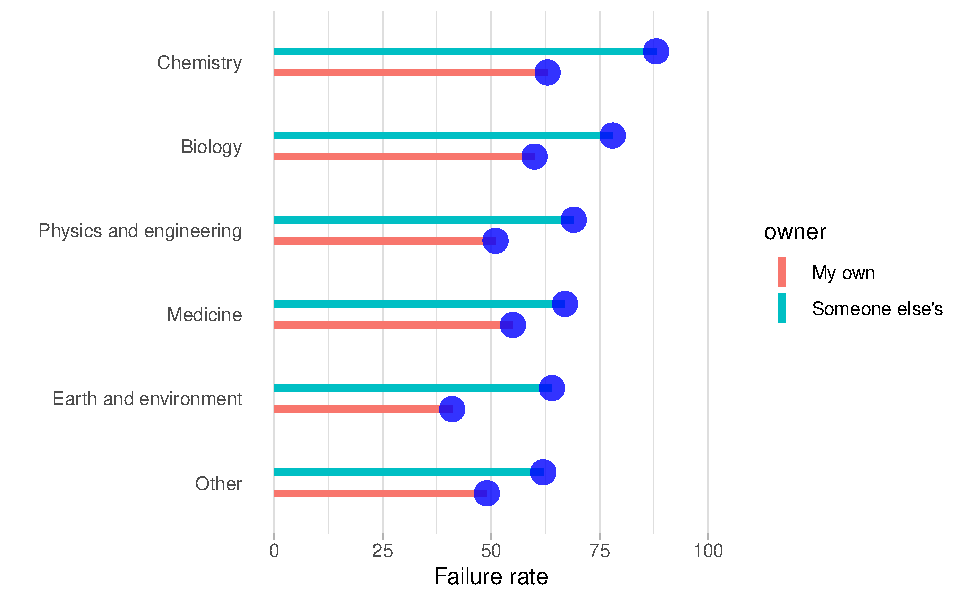
\includegraphics[width=0.9\textwidth]{figura32.pdf}
\caption{Reproducibility problems in different branches of science (data from \cite{baker20161})}
\label{figura32}
\end{figure}

\section{Characteristics of 'omic' data}
\label{sec:charomicdata}
The word "omics" makes reference to the study of some characteristics of different families of biological molecules, such as genes, proteins, etc. \parencite{palsson2002silico}. The basic aspect of the 'omic' approaches is that a complex system can be understood more thoroughly if considered as a whole. Thanks to this approach, the advances that have been achieved in the last decades in the understanding of the different biological processes are huge, and today the future of medicine and biology cannot be understood outside the view of the different 'omics' approaches \parencite{van2018role}. In few years, 'omics' technologies have given us an unimaginable deep knowledge of many cellular processes and pathways, helping the scientific community to make huge progresses in the understanding of living systems. Each year new technologies are developed allowing for the gathering of more information, increasing the resolution of the analyses and improving the precision of the determinations. As emerging fields, the different 'omics' are still expanding and defining themselves but, in a general view, 'omic' data can be classified according to the nature of the elements being analyzed. Following this approach, 5 different fields can be delimited (\autoref{figura01}), \parencite{horgan2011omic, 2018iv}:

\vspace{10pt}

\begin{itemize}
    \item Genomics: Focused at the structure, function, evolution and mapping of genomes, that is, the complete set of DNA of an organism.
    \item Epigenomics: Studies the complete set of epigenetic reversible modifications of the genome, which regulate expression.
    \item Transcriptomics: Focused at the whole set of RNA transcripts of an organism, that is, the expression of an organism's genes.
    \item Proteomics: Focused at the whole set of proteins produced or modified by an organism. Proteomics studies protein composition, structure and activity.
    \item Metabolomics: Studies metabolites in a biological entity, which are the end products of cellular processes.
\end{itemize}

\begin{figure}[htbp]\centering
		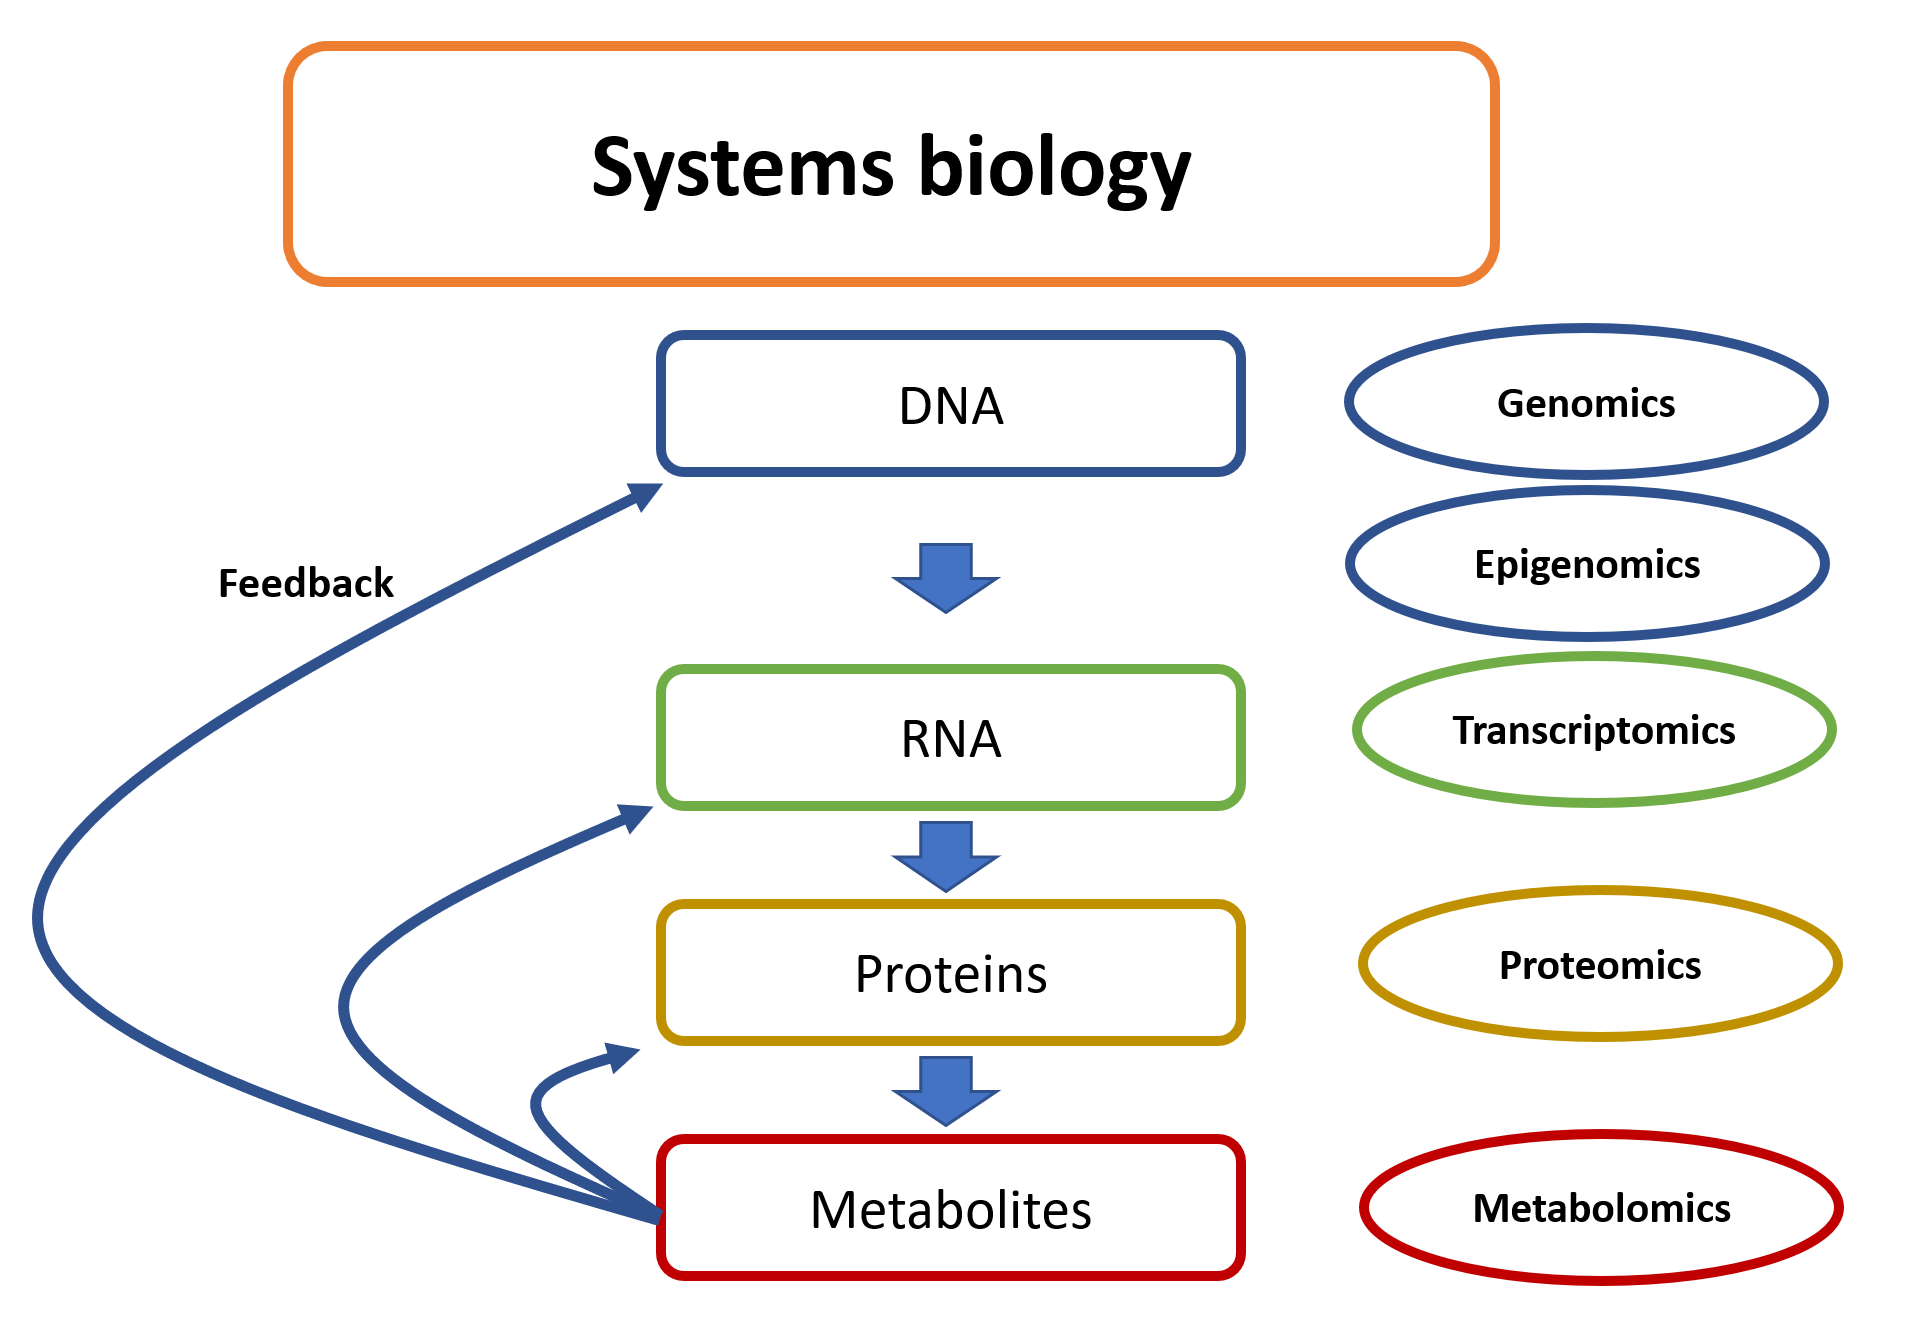
\includegraphics[width=.7\textwidth]{figura01}
		\caption{Different 'omic' technologies and their relationship}
		\label{figura01}
	\end{figure}



\subsection{Metabolomic data}
The term '\textit{metabolome}' is used to address the entire set of metabolites present in an organism and '\textit{metabolomics}' is defined as the comprehensive and quantitative analysis of all metabolites of the biological system under study \parencite{fiehn2001combining}. Metabolomics studies the downstream products of the so called "omics cascade" presented in \autoref{figura01}, so its information is influenced by the actions of genomic, epigenomic, transcriptomic and proteomic mechanisms. Because of this, metabolomics is the closest approximation to phenotype among all 'omic' technologies, thus providing  more information about the actual status of the organism than the other 'omic' technologies \parencite{beger2016metabolomics}. 

In general metabolomic studies can be classified as targeted or untargeted depending on whether the researcher measures and quantifies a specific set of known metabolites or the largest possible number of metabolites contained in a biological system \parencite{orevsivc2009metabolomics}. 
Among all 'omic' technologies, metabolomics is the most complex and heterogeneous in terms of chemical diversity. More specifically, targeted metabolomic studies focus on accurate identification and quantification of a defined set of metabolites in biological samples which was predetermined by the scientific question formulated by the researcher or, in some cases, by the size of metabolite library that is available in the software used for the analyses. On the other hand, untargeted metabolomics focuses on measuring and comparing as many signals as possible in a biological samples, and then assigning these signals to specific metabolites by using annotation databases such as HMDB \parencite{wishart2007hmdb} and Metlin \parencite{smith2005metlin}. It is important to mention that a significant portion of the detected signals cannot be identified as the metabolome is not fully annotated \parencite{viant2017close}. A typical raw data spectrum of a metabolomics analysis is presented in \autoref{figura37}.

\begin{figure}[htbp]\centering
		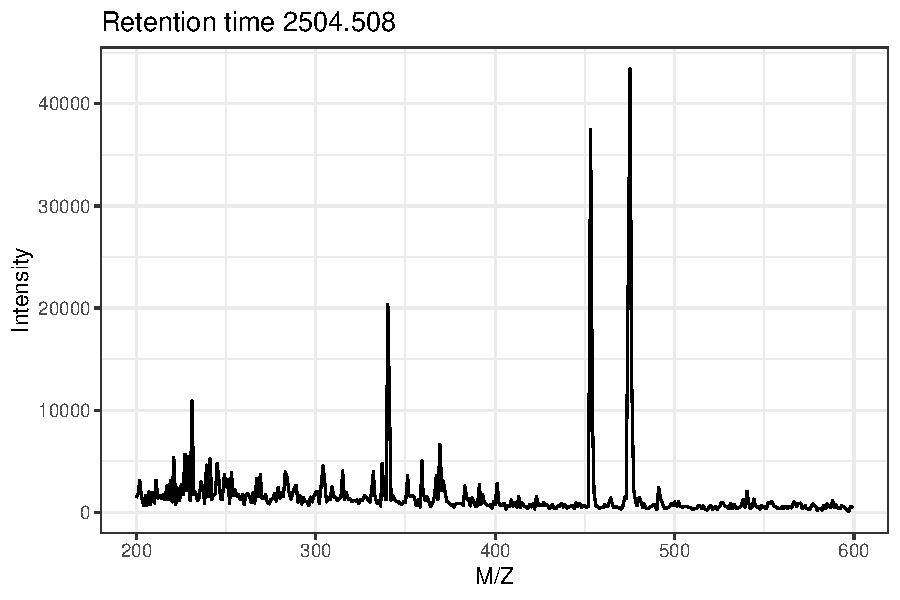
\includegraphics[width=.7\textwidth]{figura37.pdf}
		\caption{Raw spectrum of a metabolomics analysis}
		\label{figura37}
	\end{figure}

In genomics, epigenomics and transcriptomics, measurement procedures are reasonably standardized. This is not the case in metabolomics, with many different technologies being used, which lead to different study designs and different produced data types \parencite{moco2007metabolomics}. The commonly used analytical techniques for metabolomic studies are nuclear magnetic resonance (NMR), spectroscopy and mass spectrometry \parencite{buscher2009cross}. Another specific hurdle of metabolomics is the identification of the metabolites in untargeted analyses. Many of the metabolites found in an untargeted analysis can not be identified, because the data bases for associating a specific mass and retention time to a concrete metabolite are still very immature \parencite{mathew2013metabolomics}. In fact, identification of unknowns is considered as the bottleneck of untargeted metabolomics \parencite{bingol2018recent}.
In any case, although heterogeneous, metabolomic data share a common set of properties which define their most important characteristics for their statistical analysis:

\begin{itemize}
    \item High correlation among variables
    \item Complex pre-processing of the signal to obtain the data
    \item High range of detection values among variables (i.e., some metabolites are found in very small concentrations and others are found in very high concentrations)
    \item Variables (metabolites) found in one analysis are not guaranteed to be found in a subsequent analysis (i.e., lack of reproducibility).
\end{itemize}

All these properties add to the difficulty of analyzing metabolomic data, and will be further developed in the following sections.



% ---------------------------------------------------------------------
% ---------------------------------------------------------------------
% ---------------------------------------------------------------------

\chapter[Common strategies for the analysis of metabolomic data]{Common strategies for the analysis of metabolomic data}



% ---------------------------------------------------------------------
% ---------------------------------------------------------------------
\section{Classical bivariate tests}
\label{bivariate_tests}
As exposed in \autoref{sec:challengesmetabodata}, many metabolomic data analysis are performed using rudimentary statistical methods such as bivariate tests \parencite{saccenti2014reflections}. These tests, such as the well know \textit{t test} consist in the test of a specific hypothesis of equality for each of the variables being studied. The hypothesis test assesses for each metabolite if its mean (or median depending on the test being used) is different among the groups being compared. This way, in a study searching for biomarkers to discern between controls and patients of a specific disease, one hypothesis test (\autoref{hypotest}) for differences between both groups is performed for each of the metabolites in the data set, thus performing hundreds or thousands of hypothesis test in the analysis.

\begin{equation}
\label{hypotest}
\begin{split}
H_0: \mu_{controls} = \mu_{patients} \\
H_A: \mu_{controls} \neq \mu_{patients}
\end{split}
\end{equation}

The advantages of bivariate tests are the ease of application and interpretation of the results \parencite{vetter2018unadjusted}, but they suffer from a lot of issues. One of the most important issues when performing bivariate tests is the integration of results \parencite{katz2011multivariable}. Usually, even when finding several statistically significant biomarkers in a study, each of them has a small effect not being able by itself of discriminating between the groups being studied. Since the analysis was performed independenly on each variable, there is no way of combining the different selected biomarkers to perform a prediction, or even to understand the behavior of the studied biological system. Another important issue is the inability of controlling for confounders \parencite{heinze2017five}. Most sudies are observational, so groups are almost always never directly comparable. Bivariate tests are not able to take into account possible confounders and this renders many of their results invalid. There is also no way of assessing possible interactions among variables \parencite{hassall2018beyond}. As seen in \autoref{figura14}, the effect of one variable in the response can depend on the value of another. All this important information is completely lost when analyzing data one variable at a time.

\begin{figure}[hbtp]
	\centering
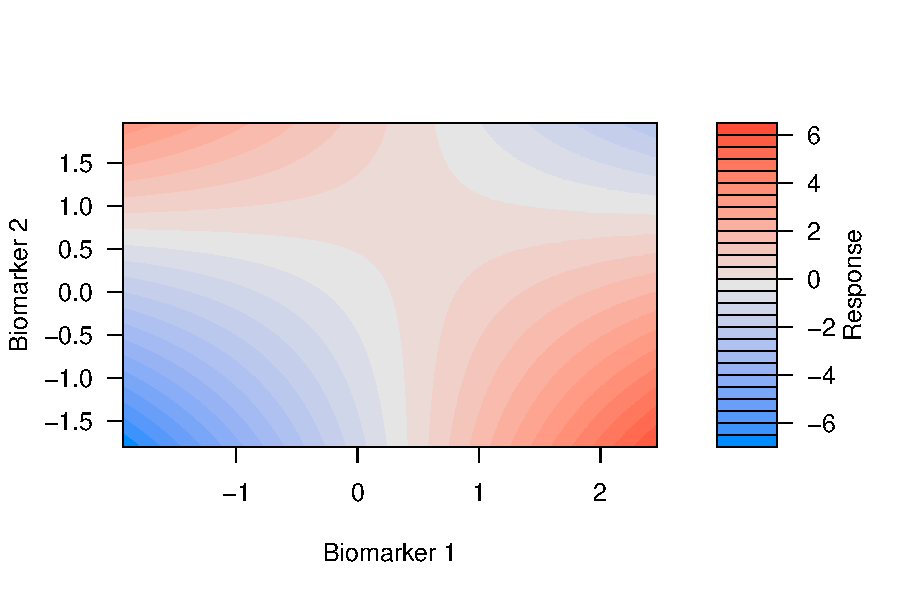
\includegraphics[width=0.75\textwidth]{figura14.pdf}
\caption[Interaction between two variables]{Interaction between two variables (biomarker 1 and biomarker 2). Higher values of one of the two biomarkers are associated to higher values of the response, but only if the other biomarker has not high values, too.}
\label{figura14}
\end{figure}

Finally, there is also a concern with the question being asked by the bivariate tests. Usually, what these analysis are doing is flipping the question. If we are looking for biomarkers for detecting a specific disease, we want to be able to predict disease with the value of the biomarkers, this is something inherently different as the question answered by the bivariate hypothesis test: Are the means (medians) for this biomarker different in each group? (\autoref{equation05}). 

\begin{equation}
\label{equation05}
\begin{split}
    Group\ {\raise.17ex\hbox{$\scriptstyle\sim$}}\ Biomarker_i \\
    vs. \phantom{MMMM}  \\
    Biomarker_i\ {\raise.17ex\hbox{$\scriptstyle\sim$}}\ Group
\end{split}
\end{equation}

In the first case, the response variable is the group and the predictors are the different biomarkers. In the second case, the responses are the different biomarkers and the predictor is the group. Since the approaches are different, it is not surprising that the fact that the means are different is not enough to achieve a good discrimination power between groups and, on the other hand, the fact that the means are equal does not mean that the biomarker is not appropriate for discriminating between groups. \autoref{figura15} shows clear examples of both cases.

\begin{figure}[hbtp]
	\centering
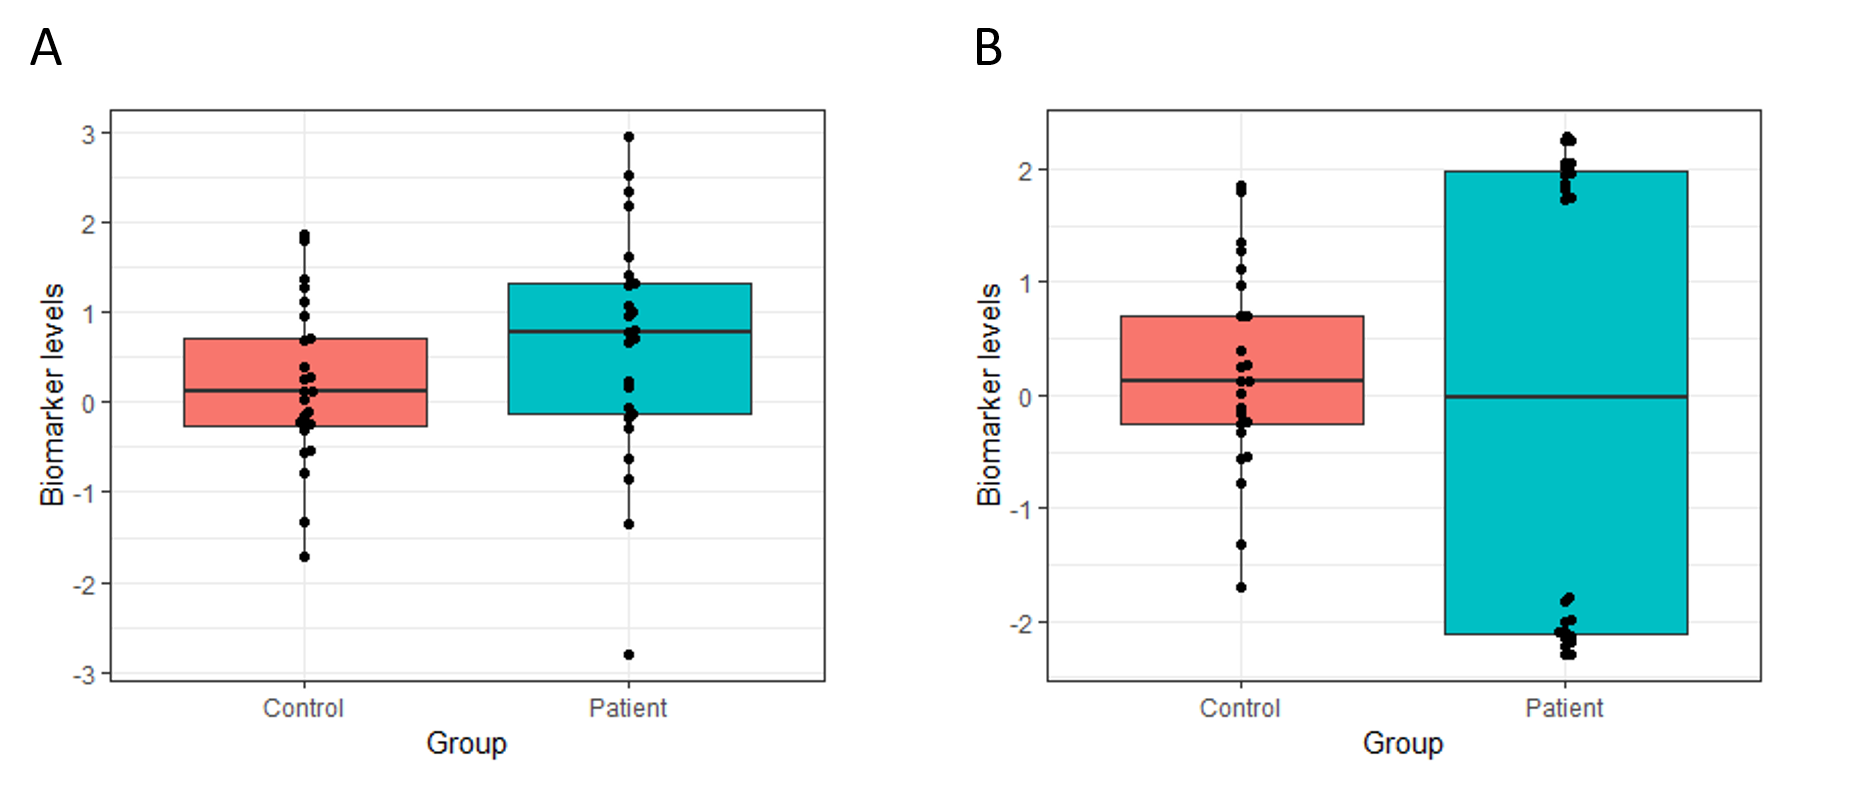
\includegraphics[width=0.95\textwidth]{figura15.png}
\caption[Difference between having different means and discrimination power]{In \textbf{A} means are different (p < 0.001) but values of the biomarker are not valid for discriminationg between controls and patients. In \textbf{B} means are exactly equal, but values of the biomarker allow for a perfect discrimination between both groups.}
\label{figura15}
\end{figure}

In summary, while compelling for their simplicity and ease of use, classical bivariate tests are not appropriate for the analysis of omic data and should only be used in the context of exploratory analysis or complementary secondary analyses.

\section{Linear modelling of omic data}
\label{linearmodels}
Linear models are a generalization of the well known statistical tests \textit{t test} and \textit{ANOVA}, where more predictors can be included in the studied association with the response variable. In fact, the standard \textit{t test} and \textit{ANOVA} are just a linear regression with one categorical predictor (\autoref{figura16})

\begin{figure}[hbtp]
	\centering
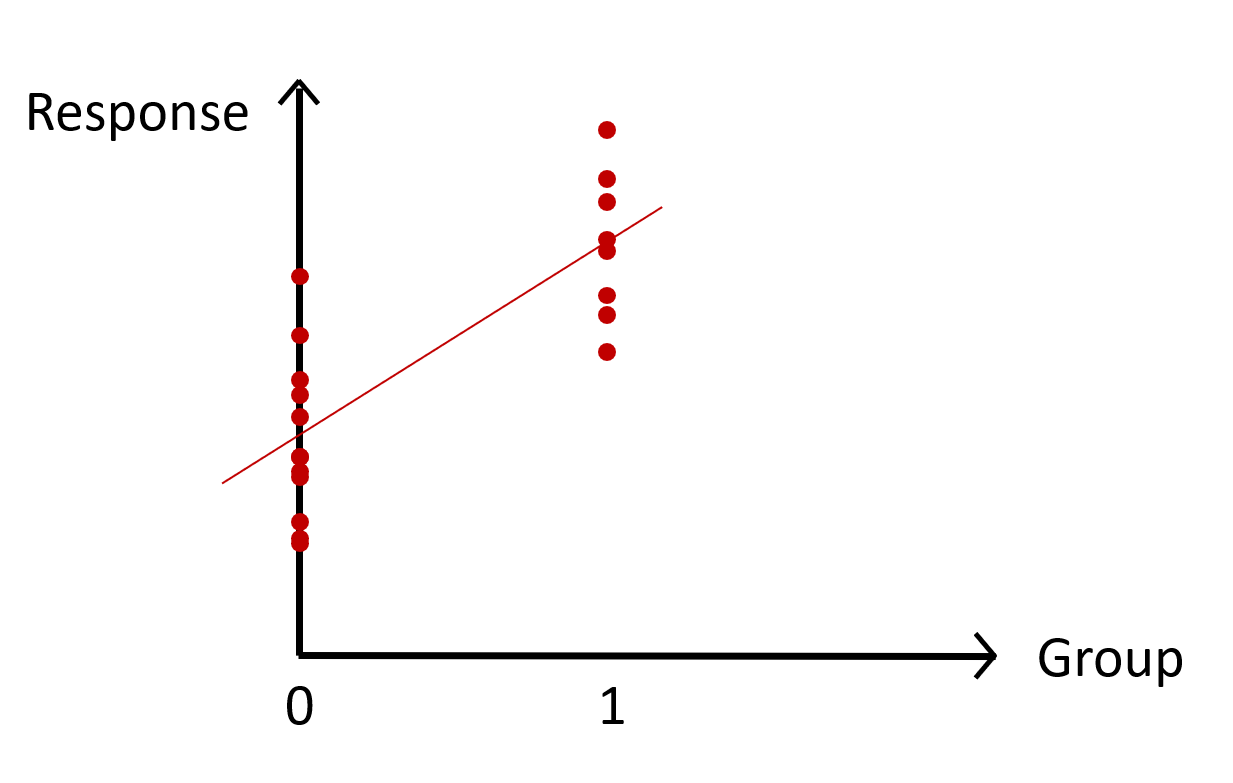
\includegraphics[width=0.75\textwidth]{figura16.png}
\caption[Equivalence between the \textit{t test} and a linear regression with one categorical predictor]{Equivalence between the \textit{t test} and a linear regression with one categorical predictor. It is easy to notice that the slope of the regression line, defined as $\Delta y/\Delta x$, equals the difference between means from group 0 and group 1.}
\label{figura16}
\end{figure}

One advantage of linear models compared to their simpler versions \textit{t test} and \textit{ANOVA} is their ability to control for confounding variables. This overcomes one of the important issues raised in \autoref{bivariate_tests} regarding non-comparable groups in observational studies. The linear model has the form showed in \autoref{equation06}. Where $\beta_0$ is the intercept and $\beta_i$ are the slopes of the different variables included in the model. The linear model can also accommodate interactions by introducing a multiplicative term between variables.

\begin{equation}
\label{equation06}
y=\beta_0 + \beta_i * x_i + \epsilon
\end{equation}

At first glance, it seems like the linear model could solve most of the problems presented in \autoref{bivariate_tests}, including integration of results, capturing interactions and answering the right question. One of the assumptions of linear models is that the response variable is continuous and has a linear relationship with the predictors, but this assumption can be relaxed using a well known generalization of the linear models known as generalized linear models \parencite{mcculloch2000generalized}. This way, it would seem possible to perform regressions to predict or explain relationships of the different metabolites with a continuous variable, and also for discriminating between different groups just by including all studied metabolites in the model as covariates. Unfortunately, linear models cannot accommodate an unlimited number of variables, because they are limited by their degrees of freedom and suffer greatly from overfitting \parencite{babyak2004you, hawkins2004problem}. Thus, in the context of omic data analysis, linear models are only useful for the control of confounding variables. This means that they are used in a similar fashion as the bivariate tests (\autoref{linearmodel}). That is, performing as many regressions as predictor variables are in the data set.

\begin{equation}
\label{linearmodel}
Biomarker_i\ {\raise.17ex\hbox{$\scriptstyle\sim$}}\ Group + Confounder + \epsilon
\end{equation}


\section{Corrections for multiple comparisons}
Each time a hypothesis test is performed, there is a $\alpha\%$ probability of a false positive (usually $\alpha = 0.05$). That means that, when using the techniques presented in \autoref{bivariate_tests} and \autoref{linearmodels}, the probability of false positives grows to unacceptable levels. The relationship between the number of performed hypothesis tests and the overall probability of a false positive is presented in \autoref{falsos_positivos}.

\begin{equation}
\label{falsos_positivos}
    Pr(False\ positive) = 1-(1-\alpha)^{n_{tests}}
\end{equation}

This entails that, in a data set with just 100 variables, we expect five false positives in average. Noteworthy, metabolomic data sets can have up to thousands of variables producing docens or even hundreds of false positives \parencite{broadhurst2006statistical}. This renders the results of the performed hypothesis tests useless, because there is no way of discriminating between false positives and true positives

\subsection{Bonferroni correction}
One method for dealing with the problem of the large number of false positives is the bonferroni correction \parencite{bland1995multiple}. In this method, the $\alpha$ value for each comparison is set to $\alpha /n_{tests}$ in order to control the family wise error rate (the probability of making one or more false discoveries, when performing all the hypothesis tests). So this method is just setting a lower threshold for the significance level. The more hypotheses are tested, the lower is the significance level threshold. This is a very basic correction, and has a major drawback: it greatly increases the number of false negatives. It is straightforward to see that only with 20 tests, the significance level is lowered to $0.05/20 = 0.0025$, so only medium to large effects will be detected assuming that sample size is large enough. But, in the case of metabolomic studies, data sets tend to have many more variables. With 500 variables, the significance level would be $0.05/500=0.0001$ and with 2000 (typical for an untargeted analysis) it would be $0.05/2000=0.000025$. Taking into account the limited sample sizes present in metabolomic studies, only the hugest effects will be detected at such a low significance level \parencite{johnson2010accounting}. 

\subsection{False Discovery Rate}
As explained in the previous paragraph, bonferroni correction greatly increases the number of false negatives. The explanation for this increase can be deduced from the pseudo formula presented in \autoref{error_rates}. In this pseudo formula, both error types are at the same place of the equation and the other parameters are fixed for a specific data set. This means that, when we decrease one of the two error types, the other has to increase accordingly.

\begin{equation}
\label{error_rates}
    N\ {\raise.17ex\hbox{$\scriptstyle\sim$}}\ \frac{variance}{effect\ size + Type\ I\ error + Type\ II\ error}
\end{equation}

In the case of bonferroni correction, the lowering of type I error is huge, so the increase in type II error is correspondingly large. In practice, this usually means that the analysis yields no positive results after a bonferroni correction. To overcome this problem, an alternative, less aggressive correction named False Discovery Rate was developed  \parencite{benjamini1995controlling}. The false discovery rate method is not concerned with the family wise error rate (FWER) as the bonferroni method. It is focused in controlling the number of false positives among all the discovered positives. So, in the case of false discovery rate, we assume that some false positives are going to happen, but want to control their proportion in relation with all the positives. The difference between this approach and the classical control of type I error is explained in \autoref{tableFDR}.

\vspace{10pt}
\begin{table}[h!]
\centering
\begin{tabular}{@{}lcc@{}}
\toprule
                         & \textbf{$H_0$ is true} & \textbf{$H_0$ is false} \\ \midrule
\textbf{Rejected $H_0$}     & FP      & TP        \\
\textbf{Not rejected $H_0$} & TN       & FN       \\ \bottomrule
\end{tabular}
\caption[Difference between FWER and FDR]{Difference between FWER and FDR. FP, TP, TN and FN stand for false positives, true positives, true negatives and false negatives, respectively. In the classic FWER procedures such as bonferroni, one is interested in maintaining the overall proportion of false positives under a specific threshold $\alpha$. In FDR, on the other hand, the interest is in maintaining the ration of FP/(FP+TP) under a specific threshold.}
\label{tableFDR}
\end{table}
\vspace{10pt}

It is easily shown that controlling the ratio FP/(FP+TP) is less stringent than controlling the overall proportion of false positives. Thus, FDR has greater statistical power, although it has a larger amount of type I error compared to bonferroni. This is expected since FDR is also subject to the formula presented in \autoref{error_rates}.

\subsection{Other corrections}
As explained in the preceding paragraph, there is no way out of the formula presented in \autoref{error_rates} when performing hypothesis tests. Several alternative methods have been provided during the last decades \parencite{benjamini2001control, gao2008multiple, castro2015adjusted}, but all of them are just playing with the balance between type I and type II error rate. Some researchers even support that the loss of power is so high, even when performing false discovery rate, that in many cases it would be better to not correct at all and consider the results as exploratory or hypotheses generators instead of forcing an unacceptable low power for confirming hypotheses \parencite{bender2001adjusting}.
In summary, hypothesis testing for the analysis of metabolomic data suffers from many issues that are difficult or, in some cases, impossible to overcome. From the exposed methods in this section, the linear modelling approach seems the most promising, specially when considering its ability to use the different metabolites as predictors, although it would have to overcome its limitation regarding overfitting and limited number of variables due to the degrees of freedom. 

\section{Principal Component analysis}
\label{sec:PCA}
It has already been exposed that linear models could be an appropriate solution for analyzing metabolomic data sets. One of the important issues with them is the saturation of their degrees of freedom when the number of variables is large. Principal component analysis (PCA) is a dimensionality reduction technique, that can be used to reduce the number of variables prior to modeling, thus helping to overcome one of the problems of linear models in the context of high dimensionality data sets \parencite{hotelling1933analysis, wang2008principal}. An illustration of the dimensionality reduction capability of PCA is provided in \autoref{figura33}.


\begin{figure}[hbtp]
	\centering
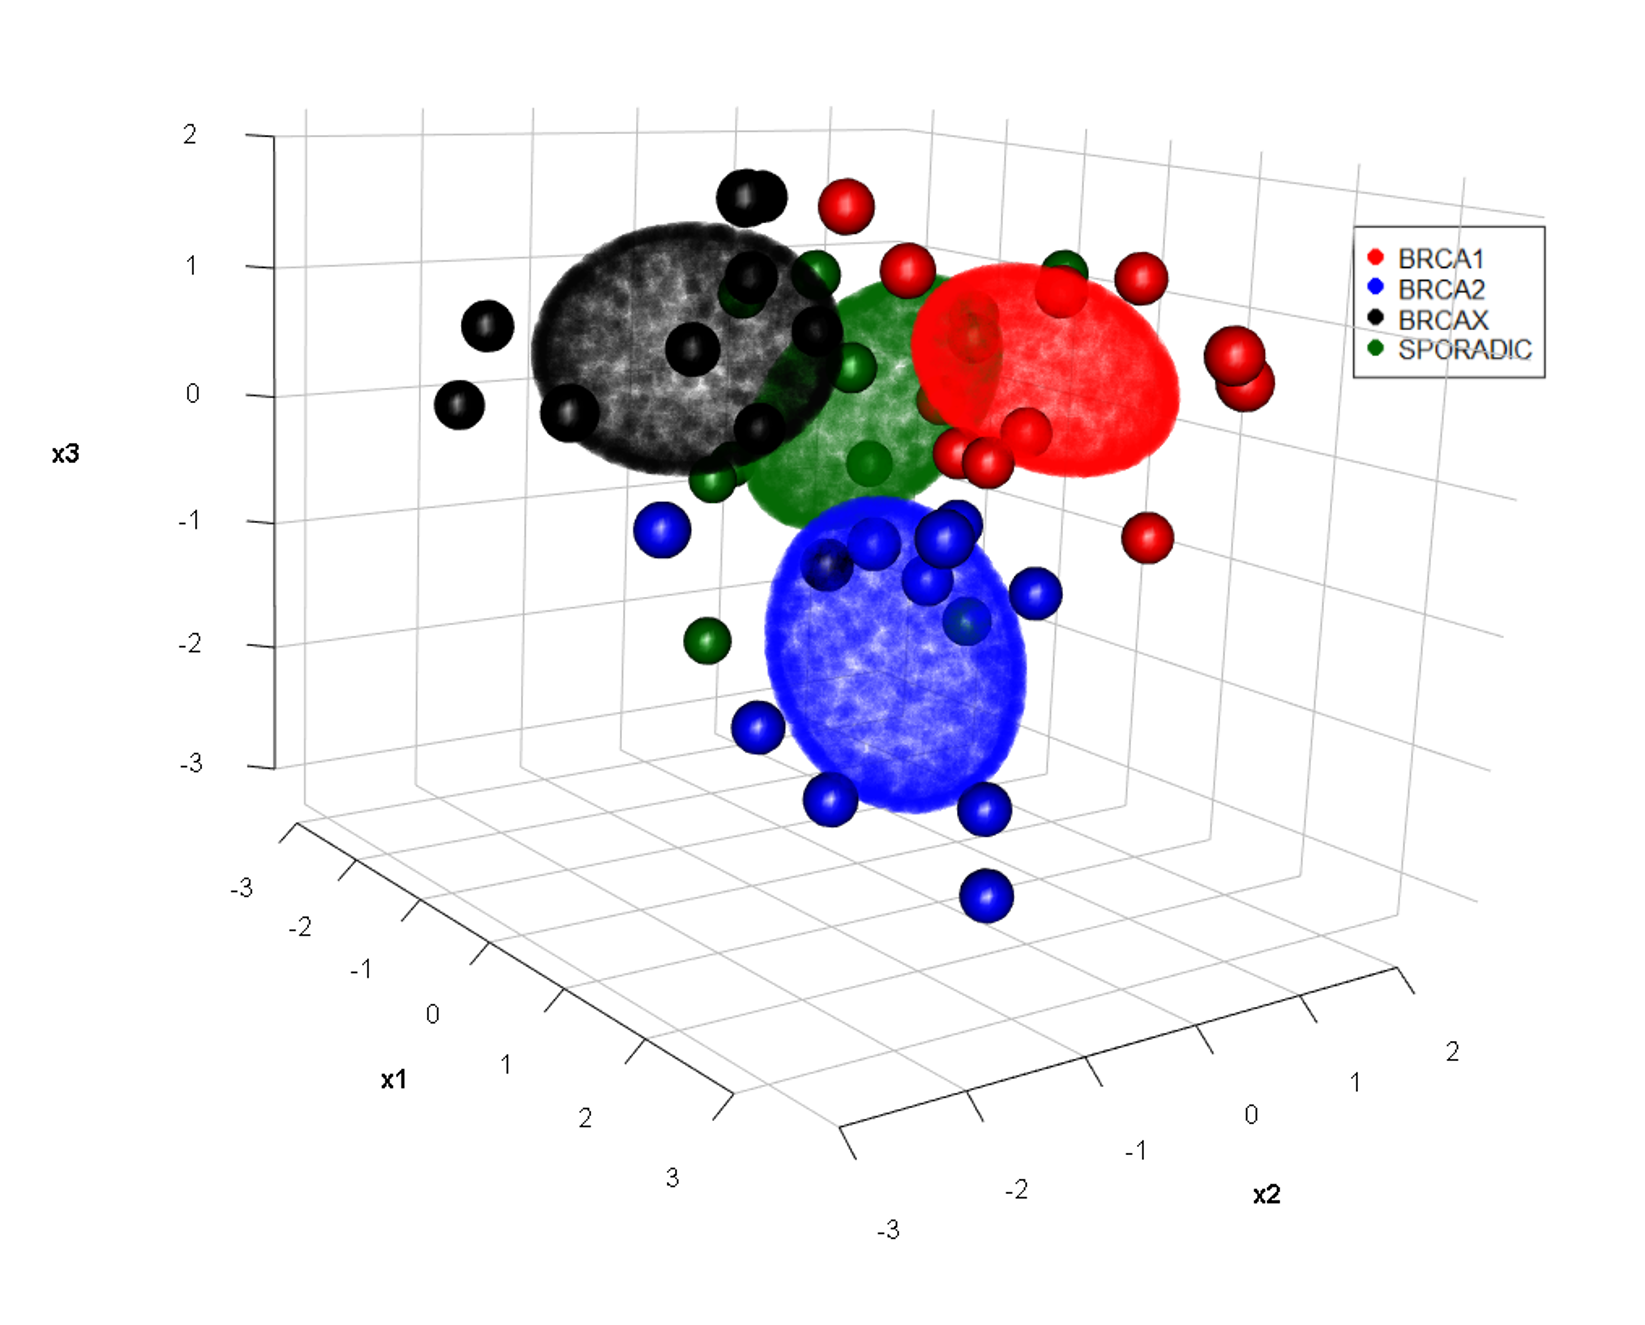
\includegraphics[width=0.75\textwidth]{figura33.png}
\caption[Plot of the first three principal components of a miRNA dataset]{Plot of the first three principal components of a miRNA dataset. These components carry enough information to be able to discriminate four different groups of samples.}
\label{figura33}
\end{figure}

Formally, PCA is defined as an orthogonal linear transformation that projects the data in a new coordinate system such that the greatest variance of the data lies in the first dimension, the second greatest variance in the second dimension, and so on until the number of components is equal to the number of original dimensions. The full principal components decomposition of \textbf{X} is given by (\autoref{equation07}).

\begin{equation}
\label{equation07}
\textbf{\text{T}} = \textbf{\text{XW}}
\end{equation}

Where \textbf{W} is a $p \times p$ matrix of weights whose columns are the eigenvectors of $\textbf{\text{X}}^T\textbf{\text{X}}$. Since the last components are the ones accounting for the least part of the variability, they carry almost no information from the original data matrix. Thus, it is reasonable to remove them keeping only the first components and effectively reducing the dimensionality of the data. Principal component regression then uses these first components as predictors in a linear regression model to predict the response \parencite{jolliffe1982note}.

Another common use of PCA is as an exploratory analysis method \parencite{tsai2007dimensionality}. Since it is very hard to represent more than three dimensions in a surface such as a sheet of paper or a screen, multidimensional data sets such as those coming from omic technologies are difficult to visualize. The dimensionality reduction produced by PCA allows for the representation of such data sets and the performing of exploratory analyses such as outlier detection, batch effect assessment, etc. \parencite{meglen1992examining}.


% ---------------------------------------------------------------------
% ---------------------------------------------------------------------
% ---------------------------------------------------------------------

\chapter[Modern techniques for the analysis of metabolomic data]{Modern techniques for the analysis of metabolomic data}
\label{chapter:modern_techniques}


% ---------------------------------------------------------------------
% ---------------------------------------------------------------------
\section{Projection based methods}
\label{projectionmethods}
In the previous chapter, the projection technique known as PCA has been introduced. As explained in section \ref{sec:PCA}, this method works by performing a dimension reduction to an original data matrix with dimensions $I \times J$, to a projected data matrix with dimensions $I \times M$, where $M<J$. Each new component of the projected data matrix is built trying to capture as much of the variability from the original data matrix as possible. So PCA is a projection technique that tries to reduce the dimensionality of the data while trying to maximize the information kept from the original data. This approach can be great for performing exploratory analysis of a data set or unsupervised analysis, but can be inefficient for performing supervised analysis such as regression or classification. The reason for this is that, while variables with the highest variability carry most of the information of the original data matrix, they do not have to be the ones able to explain the response we are trying to predict \parencite{kettaneh2005pca}. A conceptual explanation of this is presented in \autoref{figura02}.

\begin{figure}[htbp]\centering
		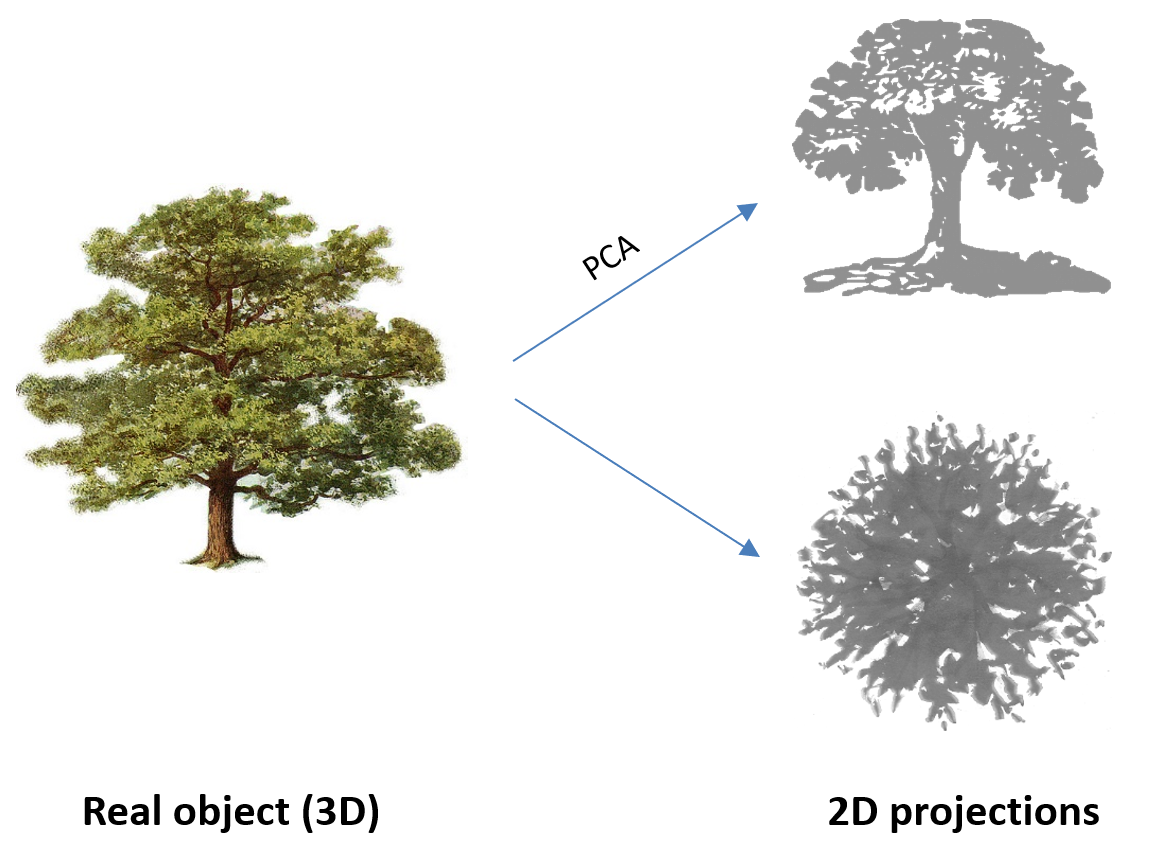
\includegraphics[width=.6\textwidth]{figura02}
		\caption{Variables with less variability can be the ones related to the response, thus being infrarepresented in the first components of PCA. In this example, if we wanted to predict the amount of shadow dropped by the tree, the PCA projection would not be efficient, while the other presented projection fully captures our target prediction. On the other hand, the PCA projection makes the tree fully recognizable, while the other projection makes it hard to even guess there is a tree.}
		\label{figura02}
	\end{figure}

Thus, if the aim is prediction, projection for maximizing the explained variability on the original data matrix is not the best approach. It is much better to maximize covariance with the response. This is how the technique Partial Least Squares (PLS) works.

\subsection{Partial Least Squares}
In linear regression, there is a limit on the number of variables that can enter a model for a specific sample size. Recent studies have shown that a minimum of two independent observations per variable are needed for estimating regression coefficients with reasonable bias \parencite{austin2015number}. Metabolomic data sets usually have many more variables than observations, so linear regression models are not a viable alternative for analyzing these data sets. Linear regression also suffers from multicollinearity, so when highly correlated predictors are used together in a model their coefficients get unstable and standard errors grow wildly \parencite{alin2010multicollinearity}. PLS can be seen as an extension of multiple linear regression designed to overcome the issues just described. It can analyze data sets with strongly correlated variables and handle situations where the number of variables far exceeds the number of observations \parencite{wold2001pls}. Additionally, PLS can also simultaneously model several response variables. It is important to note that results of PLS (and of projection methods in general) depend on the scaling of the data so, before the analyses, the \textbf{X} and \textbf{Y} variables are often scaled to unit variance and centered to the mean.
A scheme of the PLS model is depicted in \autoref{figura17}.

\begin{figure}[hbtp]
	\centering
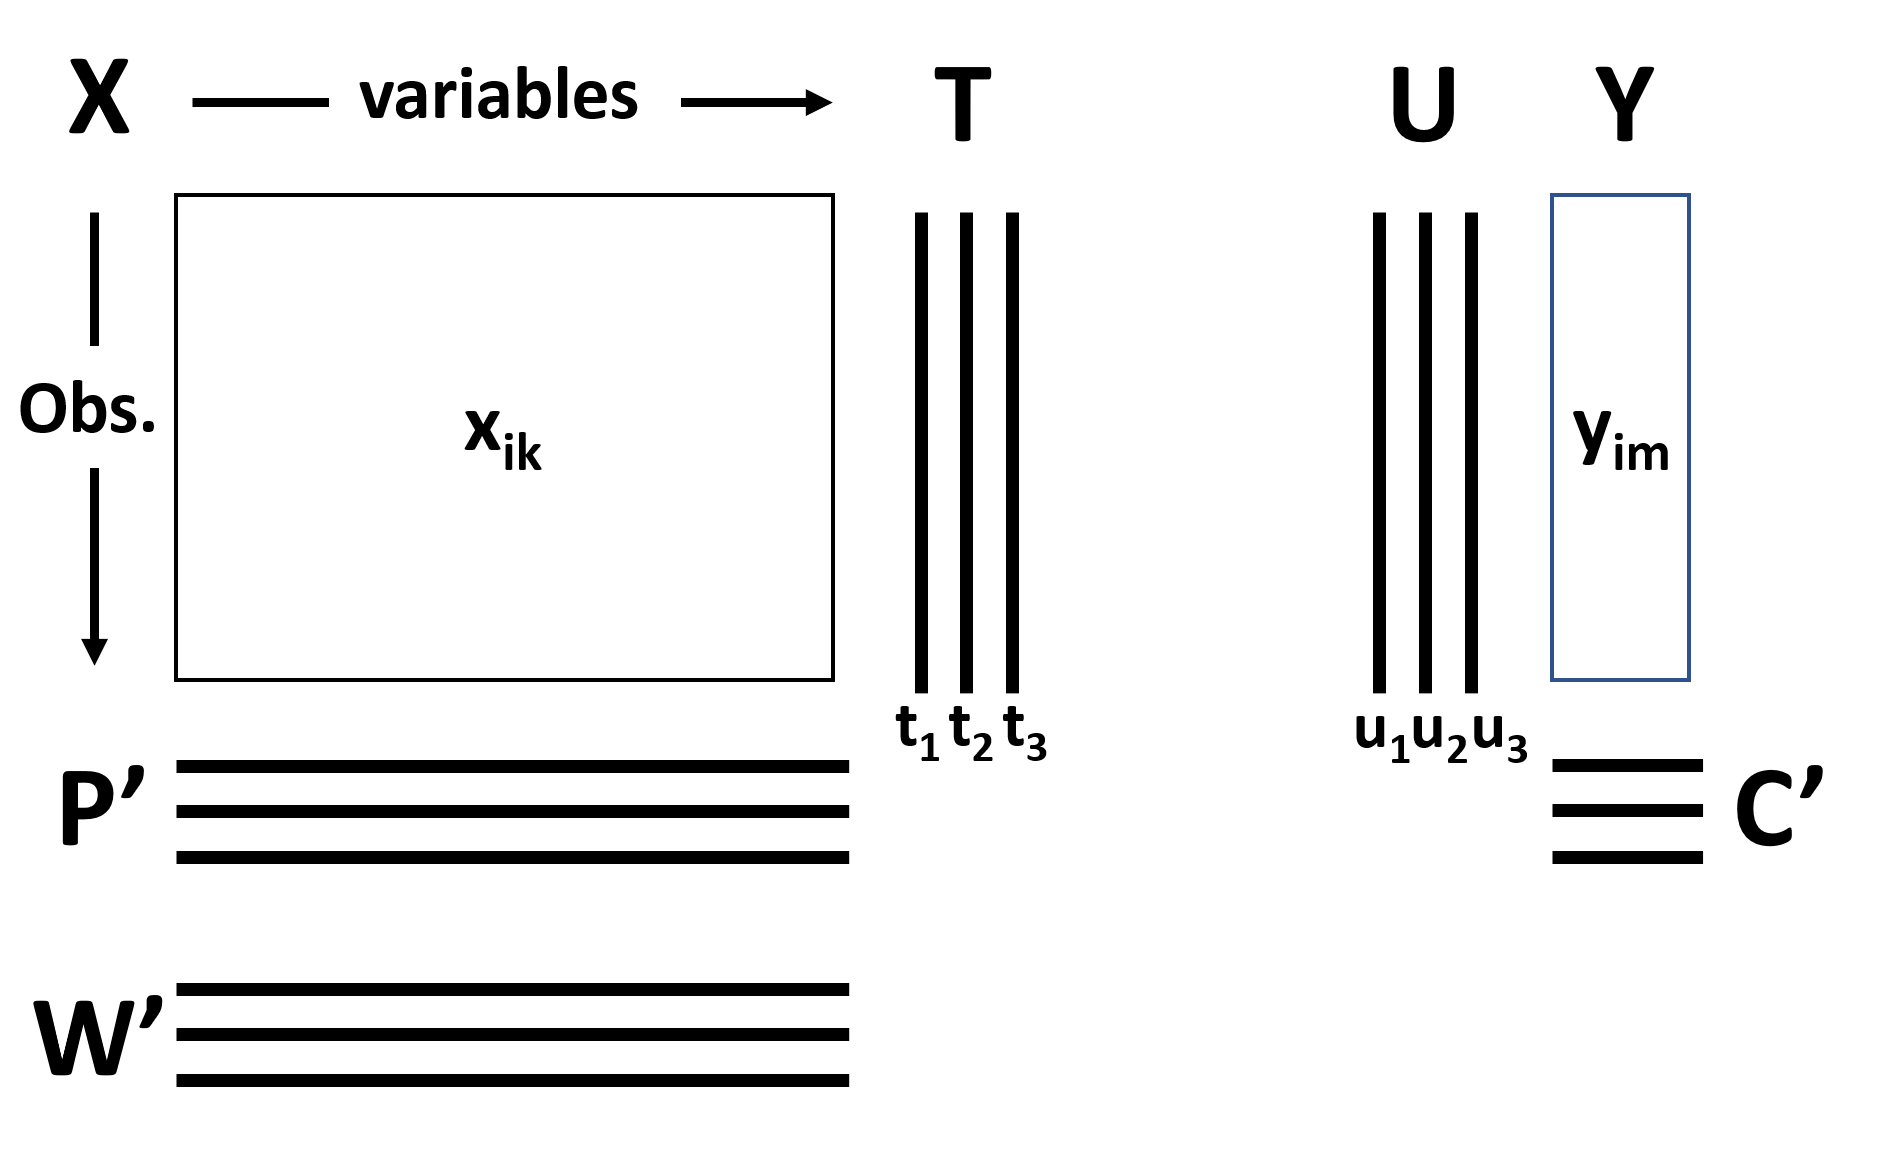
\includegraphics[width=0.7\textwidth]{figura17.png}
\caption{Scheme of the PLS model \parencite{wold2001pls}. \textbf{X} is the matrix of predictors and \textbf{Y} is the matrix of responses. Additional matrices are generated at the different modelling steps.}
\label{figura17}
\end{figure}

The PLS model finds latent variables (denoted by $\text{t}_a$, where a = 1, 2, \dots, A) that are predictors of \textbf{Y} and also model \textbf{X}. These latent variables are also called X-scores and are orthogonal. They are estimated as linear combinations of the original variables using different weights denoted by $\text{w}^*_{ka}$ (\autoref{equation08}). 

\begin{equation}
\label{equation08}
\textbf{\text{T}}=\textbf{\text{XW}}^*
\end{equation}

X-scores are multiplied by the loadings $\text{p}_{ak}$ minimizing residuals in \textbf{X}, denoted as \textbf{E} (\autoref{equation09}).

\begin{equation}
\label{equation09}
\textbf{\text{X}}=\textbf{\text{TP}}'+\textbf{\text{E}}
\end{equation}

Analogously, the Y-scores are multiplied by the weights (denoted by $\text{c}_{am}$) minimizing residuals in \textbf{Y}, denoted as \textbf{G} (\autoref{equation10}).

\begin{equation}
\label{equation10}
\textbf{\text{Y}}=\textbf{\text{UC}}'+\textbf{\text{G}}
\end{equation}

As stated before, X-scores are good predictors of \textbf{Y} (\autoref{equation11}).

\begin{equation}
\label{equation11}
\textbf{\text{Y}}=\textbf{\text{TC}}'+\textbf{\text{F}}
\end{equation}

Where \textbf{F} is the residuals matrix from \textbf{Y}. Alternatively, \autoref{equation11} can be rewritten as follows (\autoref{equation12}):

\begin{equation}
\label{equation12}
\textbf{\text{Y}}=\textbf{\text{XW}}^*\textbf{\text{C}}'+\textbf{\text{F}}=\textbf{\text{XB}}+\textbf{\text{F}}
\end{equation}

Which resembles a multiple linear regression model where the predictors matrix \textbf{X} is multiplied by the coefficients matrix \textbf{B} to predict \textbf{Y}.

With PLS, we have introduced a modelling technique able to effectively deal with metabolomic data. Correlated variables and data sets with many more variables than observations can be properly analyzed and results are easily interpreted with the help of useful plots of the scores, loadings and predictions of the model (\autoref{figura18}).

\begin{figure}[hbtp]
	\centering
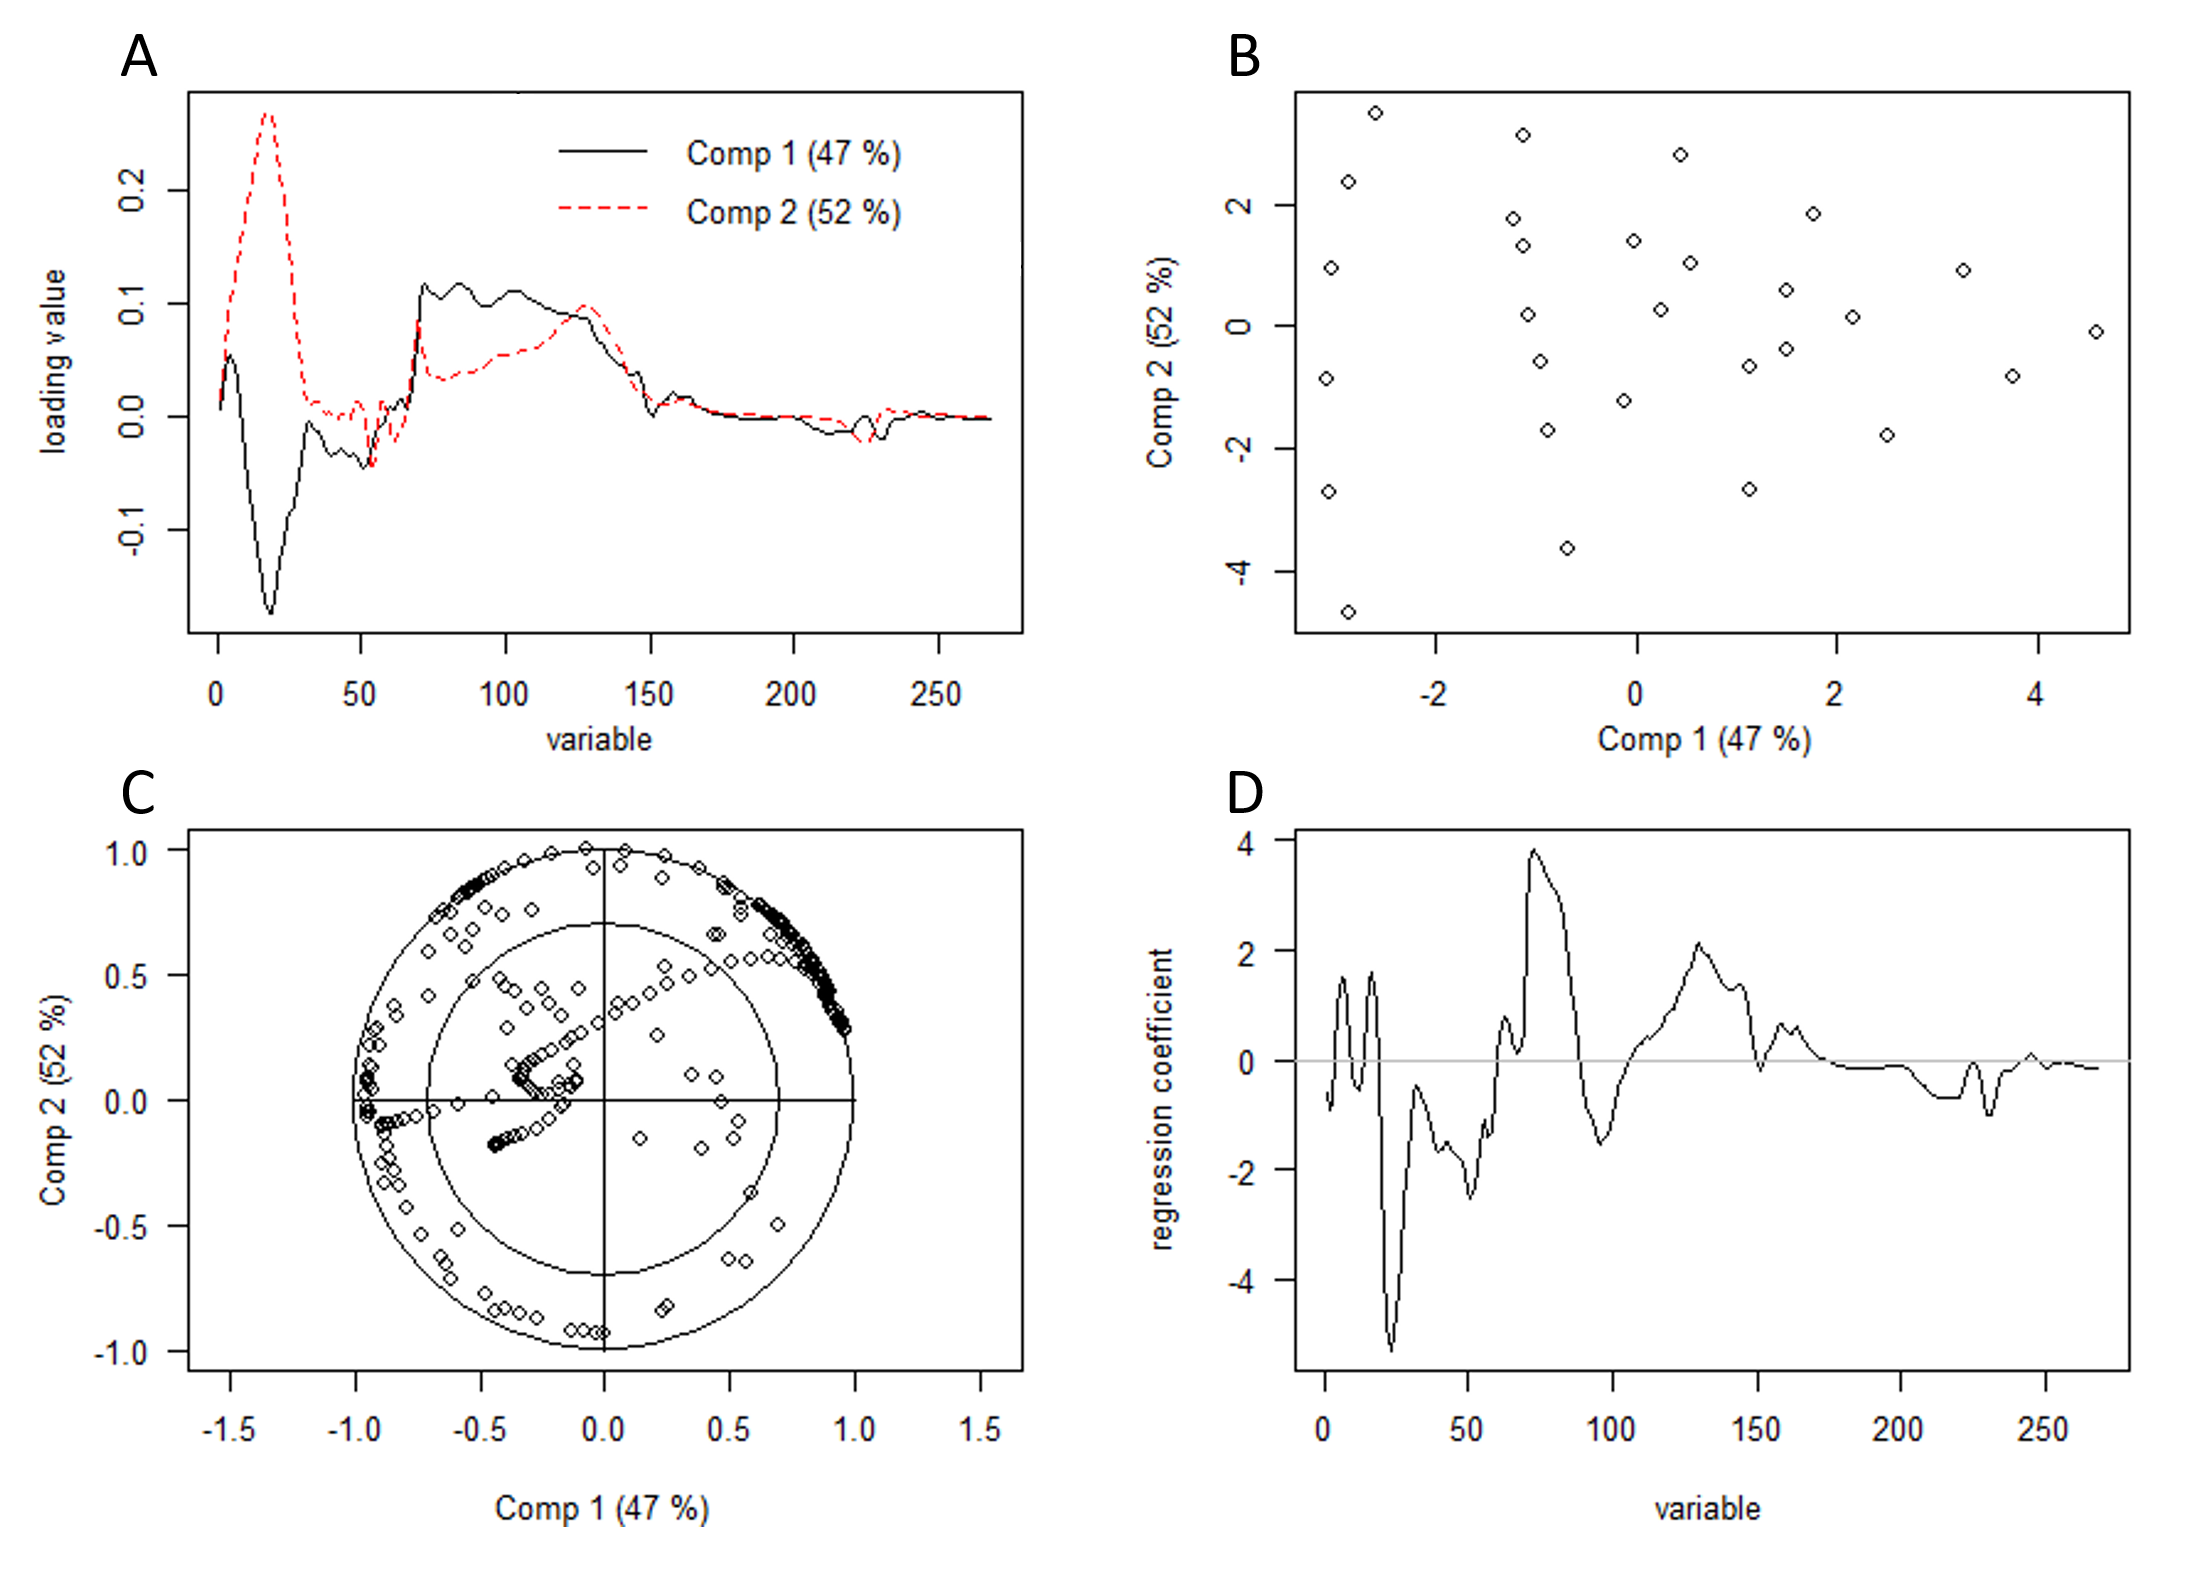
\includegraphics[width=0.82\textwidth]{figura18.png}
\caption{Plots of a PLS model. \textbf{A} shows the loadings for each variable in the two first components. \textbf{B} shows the scores for each observation in the first two components. \textbf{C} represents the correlations between each variable and the first two components.  \textbf{D} shows the regression coefficients of the model.}
\label{figura18}
\end{figure}


\section{Penalization methods}
\label{penalmethods}
Another set of techniques able to deal with metabolomic data sets are the penalization methods. These methods are motivated by the relationship between model complexity and prediction error, also known as bias-variance trade-off \parencite{hastie2001model}. As depicted in \autoref{figura19}, prediction error in the same data set used to fit a specific model always decreases when increasing the complexity of the model. On the other hand, prediction error in new data decreases at first, reaching a minimum at a specific model complexity, and increases later again as model complexity keeps growing larger.

\begin{figure}[hbtp]
	\centering
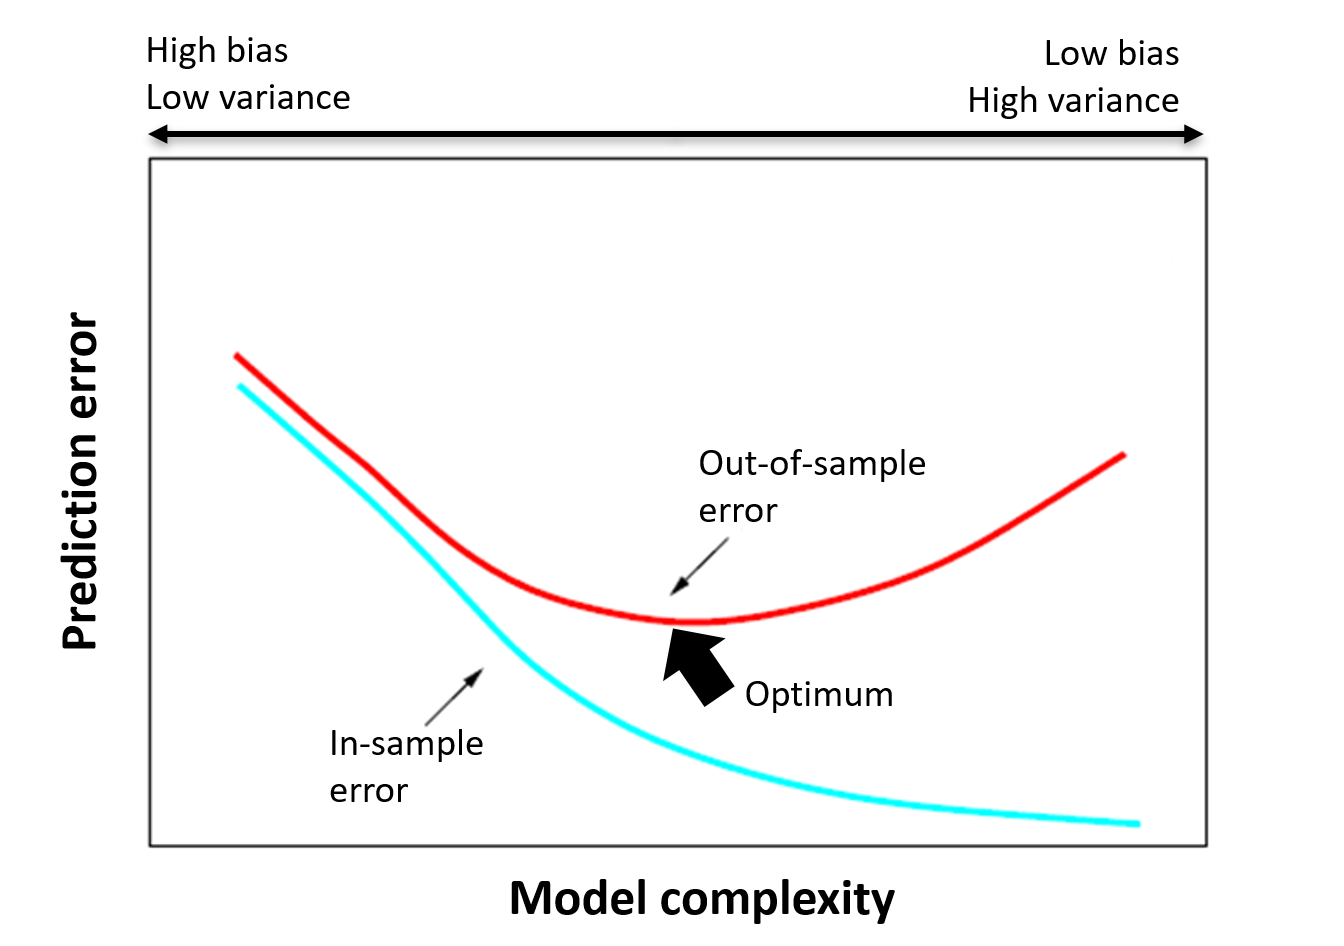
\includegraphics[width=0.75\textwidth]{figura19.png}
\caption{Behavior of prediction error in training (in-sample) and test (out-of-sample) data.}
\label{figura19}
\end{figure}

As previously described, metabolomic data sets are characterized by having a large number of variables and relatively a low number of observations. Trying to fit a model with all the variables in this situation would correspond to the extreme right side of the plot in \autoref{figura19} with low bias and high variance. This is the reason why multiple regression models cannot be fit to these data, variance grows to infinite as the number of predictor variables increases in the model. But this relationship between bias-variance and model complexity gives us the key for improving the standard linear models: increasing bias will reduce the variance, potentially obtaining a lower out-of-sample prediction error because model complexity has been decreased. Thus, the solution for being able to fit linear models to metabolomic data is to bias them. The full reasoning behind this last sentence can be better understood with the explanation provided in \autoref{figura20}.

\begin{figure}[hbtp]
	\centering
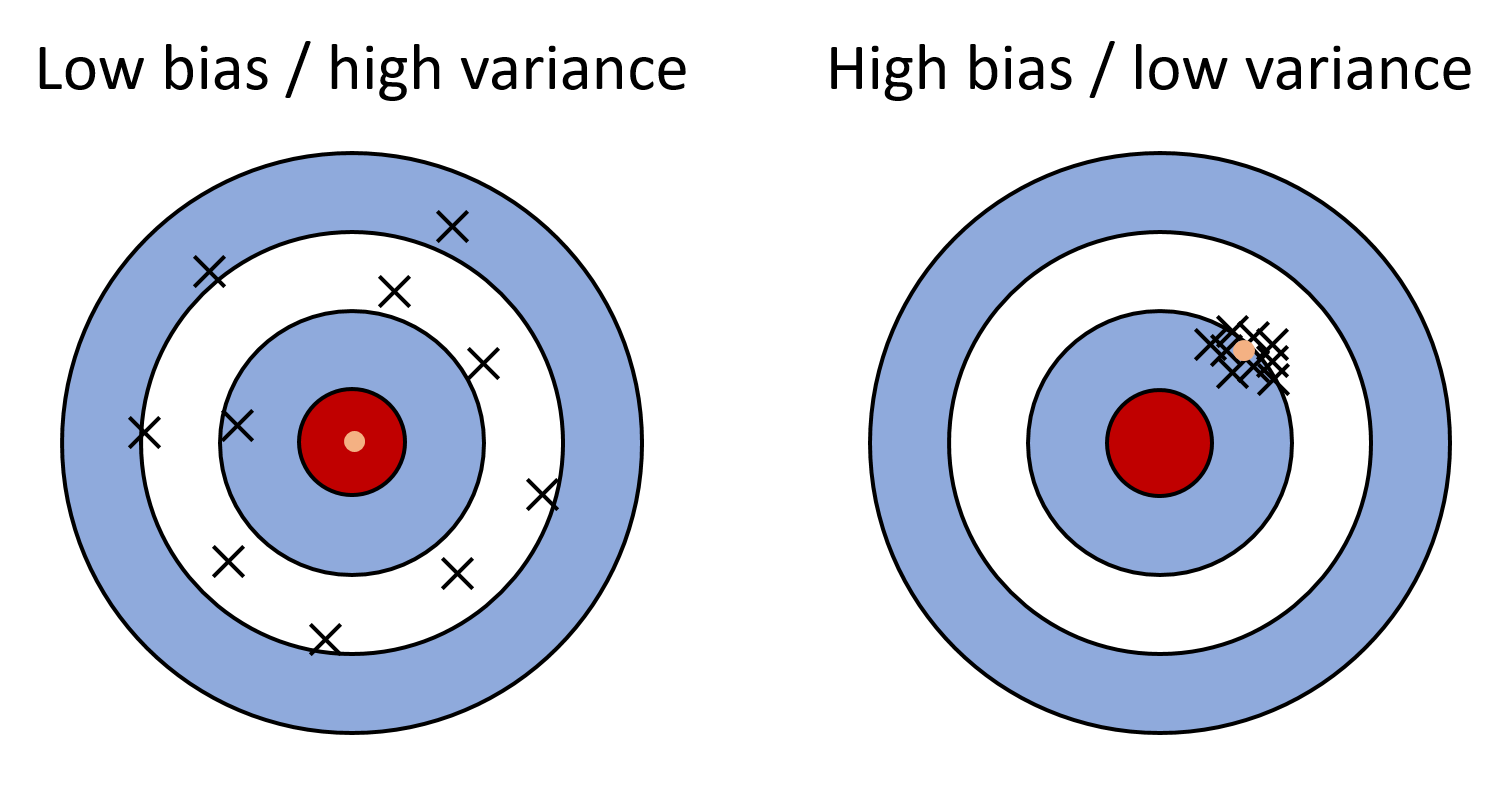
\includegraphics[width=0.75\textwidth]{figura20.png}
\caption{In both targets each black cross represents an estimation of a specific model to different samples of the same population and the orange dot represents the average estimation of all of them. In the left target there is no bias, with the orange dot right at the bullseye, but estimation from the different samples are wildly spread with a very high variability. In the right target, there is a perceptible amount of bias, the orange dot lies out of the bullseye, but all estimations from the different samples are concentrated in a small area around the average estimation. Usually, only one sample (one data set) is available for performing the estimation, so the advantage of introducing bias to lower variance is evident.}
\label{figura20}
\end{figure}

\subsection{Ridge regression}
The first developed penalization method for linear regression was ridge regression \parencite{hoerl1970ridge}. This method consists in solving the ordinary least squares problem, but introduces a restriction to the solution. This restriction consist in setting an upper bound on the sum of the squared coefficients (L2 norm) (\autoref{equation13}).

\begin{equation}
\label{equation13}
\begin{split}
\hat{\beta}^{ridge}=\argmin_\beta \sum\limits_{i=1}^N (y_{i}-\beta_{0}-\sum\limits_{j=1}^p x_{ij}\beta_{j})^{2} \\
\textrm{Subject to the restriction:}  \sum\limits_{j=1}^p \beta_{j}^2\leq s
\end{split}
\end{equation}

The inclusion of this restriction to the ordinary least squares problem imposes a reduction in the value of the coefficients, thus biasing their estimation and producing a reduction in the complexity of the model. A graphical explanation of the functioning of the method is represented in \autoref{figura21}.

\begin{figure}[hbtp]
\centering
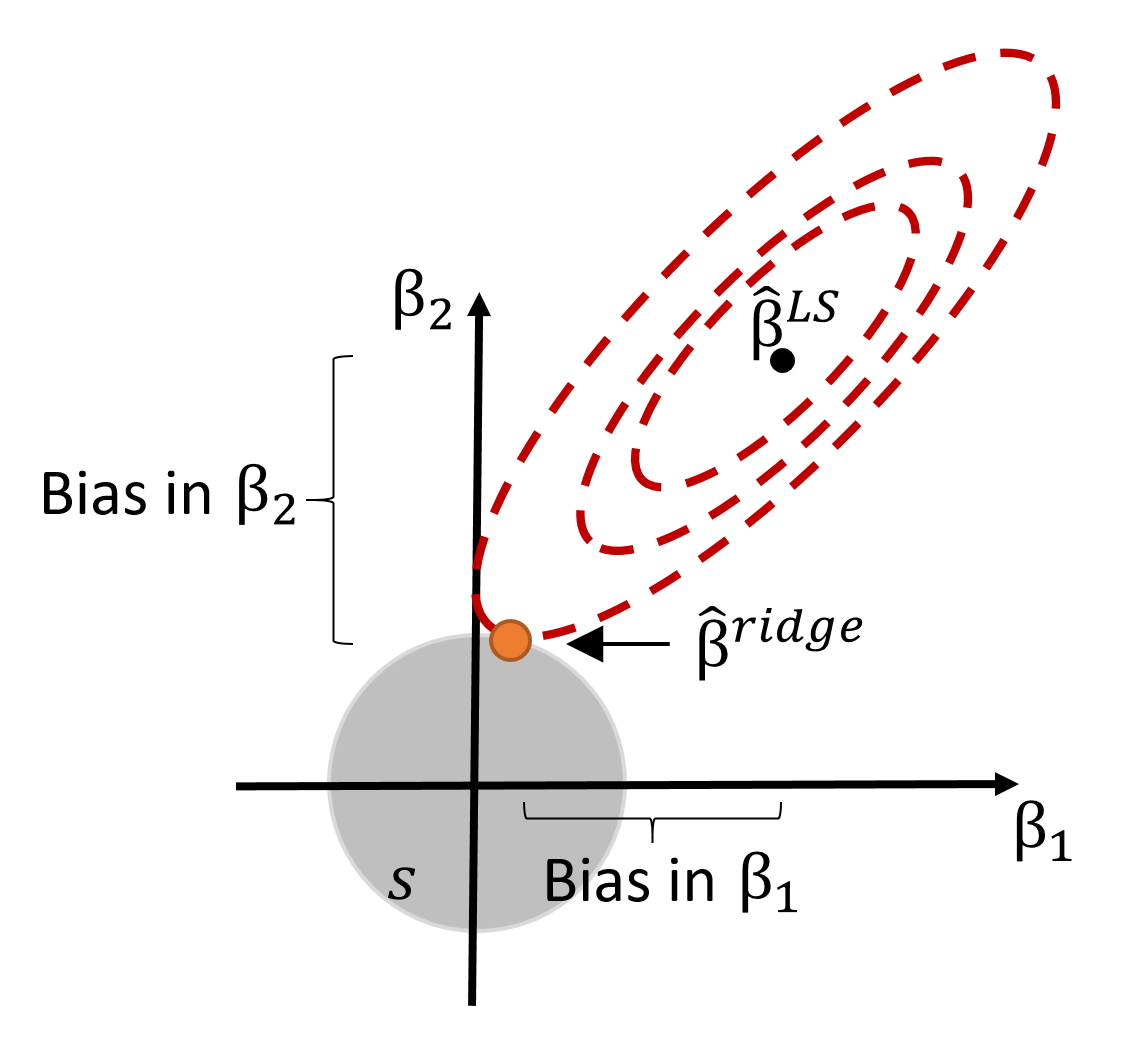
\includegraphics[width=0.6\textwidth]{figura21.png}
\caption{Ridge regression for a linear model with two predictors. As the restriction is intensified (lower value of $s$), the estimation of the coefficients is more biased to zero. Dashed red lines represent least squares contour lines. Grayed area represents the restriction imposed by $s$.}
\label{figura21}
\end{figure}

The solution offered by ridge regression is very similar to that obtained by PLS. A regression model suitable for metabolomic data sets with many, highly correlated variables. Both methods use all the variables for adjusting the model and both models shrink the estimates of the coefficients \parencite{de1995pls}, thus reducing model complexity and therefore variance at a cost of increasing bias.

\subsection{Lasso}
\label{lasso}
In many studies it is the case that it is not only of interest fitting a predictive model, but also selecting the most important predictors among all the variables present in the data. As has been exposed in the previous sections, neither PLS nor ridge regression provide a direct method for variable selection. They both use all the variables in the data set for adjusting the model. It is true that there are some post-model-fitting methods for assessing variable importance in the case of PLS \parencite{mehmood2012review}, but they require and additional filtering step after the model has been fitted and are not inherent to the PLS model. The method known as lasso is similar to ridge regression. But instead of setting a bound on the sum of the squared coefficients, it is set on the sum of the absolute values of the coefficients (L1 norm) as seen in \autoref{equation14} \parencite{tibshirani1996regression}. This change in the method of penalization of the coefficients allows that some of them are set to zero when the model is adjusted, thus producing a variable selection at the model-fitting step.

\begin{equation}
\label{equation14}
\begin{split}
\hat{\beta}^{lasso}=\argmin_\beta \sum\limits_{i=1}^N (y_{i}-\beta_{0}-\sum\limits_{j=1}^p x_{ij}\beta_{j})^{2} \\
\textrm{Subject to the restriction:}  \sum\limits_{j=1}^p |\beta_{j}|\leq s
\end{split}
\end{equation}

\autoref{figura22} shows how increasing the penalization by reducing $s$ forces the parameters to zero, producing a simpler model by deselecting some features. Thus, assuming data are standardized, Lasso automatically selects the most relevant features and discards the others.

\begin{figure}[hbtp]
\centering
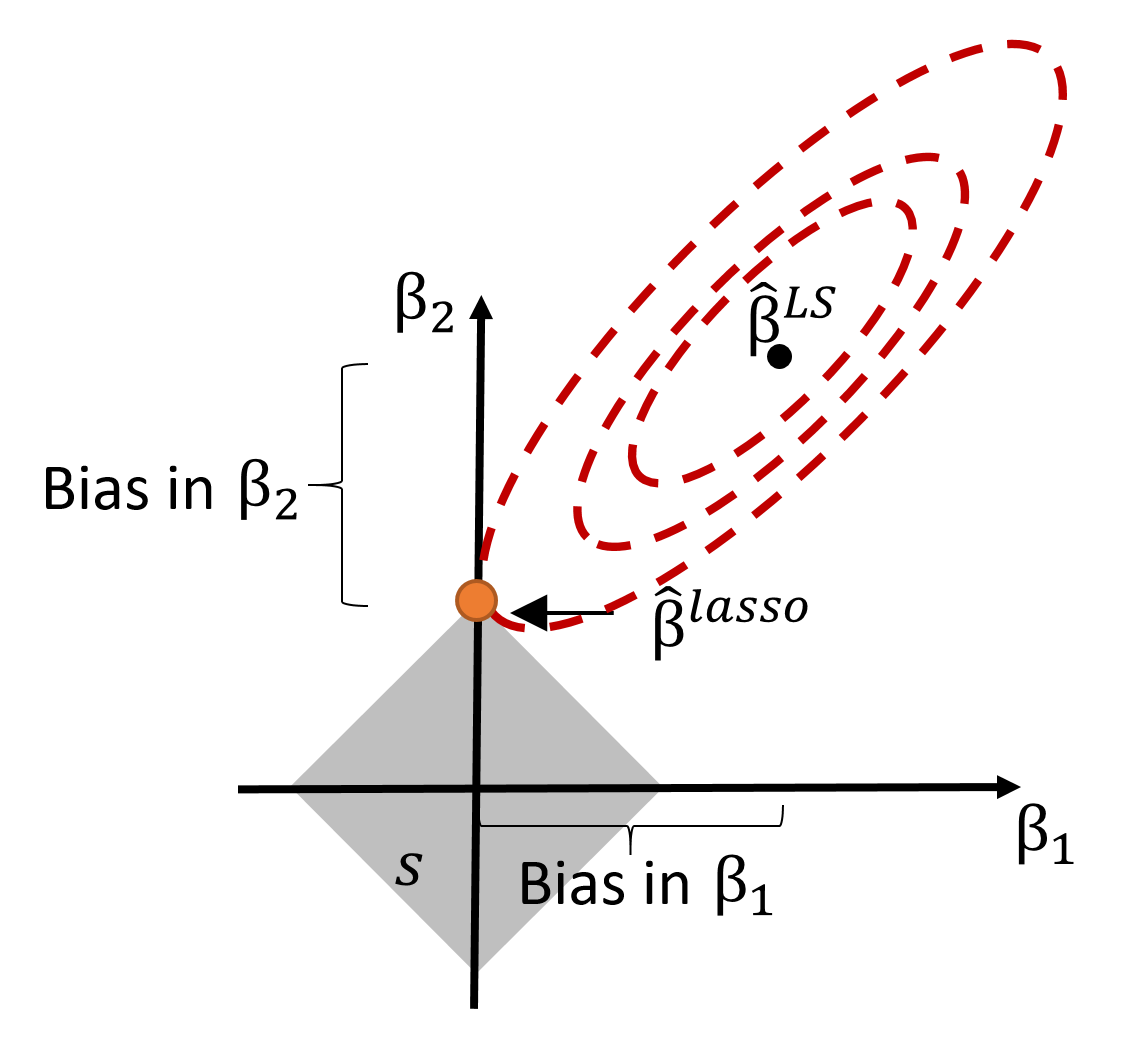
\includegraphics[width=0.6\textwidth]{figura22.png}
\caption{Lasso regression for a linear model with two predictors. As the restriction is intensified (lower value of $s$), the estimation of the coefficients is more biased to zero. Since it is more easier to land in a vertex than in an edge, reducing $s$ forces one of the coefficients to zero. Dashed red lines represent least squares contour lines. Grayed area represents the restriction imposed by $s$.}
\label{figura22}
\end{figure}

The fact that lasso allows for variable selection makes it a very appealing solution for modelling omic data. Unfortunately, unlike PLS and ridge regression, lasso is not able to deal with multicollinearity in an optimal manner \parencite{chong2005performance}, which is a prominent characteristic of metabolimic data. When two (or more) variables are highly correlated, lasso will select one of them discarding the others and, potentially, losing predictive performance and important variables.

\subsection{Elastic net}
Two different penalization methods have been presented, each one with its own benefits and drawbacks. Ridge is able to deal with multicollinearity but does not perform variable selection and lasso performs variable selection but does not deal adequately with multicollinearity. The elastic net algorithm was developed in order to merge the good qualities of ridge and elastic net and overcome their issues \parencite{zou2005regularization}. It is a flexible combination of the two constrains defined for ridge and lasso. The L1 penalty provides variable selection and the L2 penalty provides stability in the selection of correlated variables. The balance between both penalties is defined by the parameter $\alpha$  (\autoref{equation15}). When $\alpha=0$, elastic net is equivalent to ridge regression, since the L1 constraint is set to zero. On the other hand, when $\alpha=1$, elastic net is equivalent to lasso, since the L2 constraint is set to zero. Values between $\alpha = 0$ and $\alpha = 1$ provide different balances between L1 (more variable selection) and L2 (better handling of multicollinearity) penalizations.

\begin{equation}
\label{equation15}
\begin{split}
\hat{\beta}^{elastic net}=\argmin_\beta \sum\limits_{i=1}^N (y_{i}-\beta_{0}-\sum\limits_{j=1}^p x_{ij}\beta_{j})^{2} \\
\textrm{Subject to the restriction: }  \alpha \sum\limits_{j=1}^p |\beta_{j}| + (1-\alpha) \sum\limits_{j=1}^p \beta_{j}^2 \leq s
\end{split}
\end{equation}

\autoref{figura23} depicts the elastic net in a two-variable case and shows how, while keeping the vertices present in lasso, the edges are convex and allow for grouped selection of correlated variables. This is a very attractive solution for the modelling of metabolomic data sets and has been used widely during the last years \parencite{lankinen2010dietary, bowling2014analyzing, liu2015high, ferrario2016mortality}. The only drawback of elastic net compared to lasso and ridge is the inclusion of another parameter in the model. Instead of optimizing only for the value of $s$, elastic net models have also to optimize for the value of $\alpha$, thus requiring more tuning for an appropriate fitting of the data. 

\begin{figure}[hbtp]
\centering
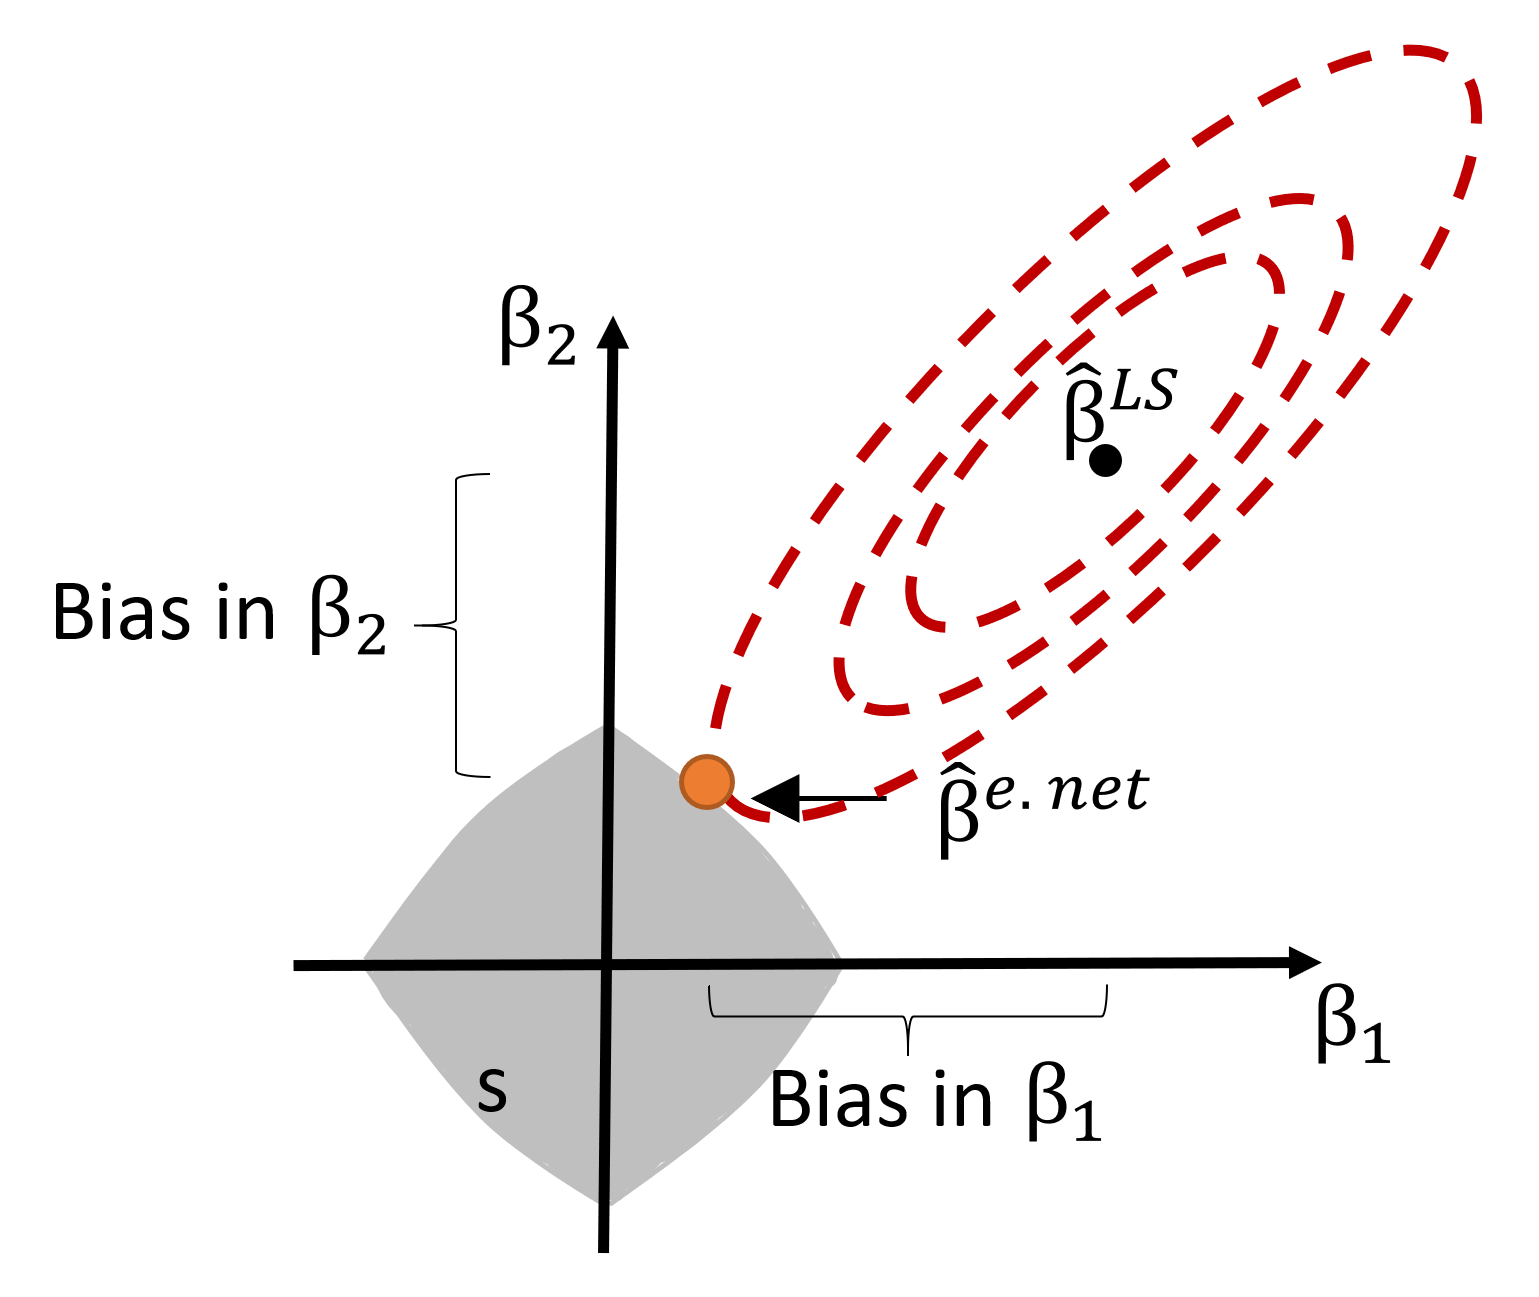
\includegraphics[width=0.6\textwidth]{figura23.png}
\caption{Elastic net regression for a linear model with two predictors. As the restriction is intensified (lower value of $s$), the estimation of the coefficients is more biased to zero. As in lasso, it is more easier to land in a vertex than in an edge, so many coefficients can be potentially set to zero. But, as in ridge, edges are convex, so highly correlated variables will be selected together. Dashed red lines represent least squares contour lines. Grayed area represents the restriction imposed by $s$.}
\label{figura23}
\end{figure}

\section{Tree-based methods}
Projection based methods and penalization methods are extensions of the standard linear model and can also be extended to generalized linear models and survival models without much effort \parencite{nygaard2008partial, simon2011regularization}. But, in essence, they are parametric models, which means that they are sensitive to outliers \parencite{liebmann2010robust, park2016robust} and that they are limited in the types of relationships among variables they can detect. Their validity is also dependent on assumptions that can or cannot be met depending on the population being analyzed. In contrast, tree-based methods are fully non-parametric methods, so they do not have underlying assumptions to be met. They were developed from an algorithmic perspective instead of from an statistical theory perspective, so many of their statistical theoretical foundations where elaborated after their development as data analysis techniques, instead of before, as is usual with most statistical methods \parencite{breiman2001statistical}. The main difference between these two approaches lies in the interpretation of the data generating process. In one case, the data is assumed to be generated by a stochastic data model which we reproduce and use to make the analysis, in the other case the data generating process is treated as unknown and algorithms are generated based in their prediction capability (\autoref{figura24}).

\begin{figure}[hbtp]
\centering
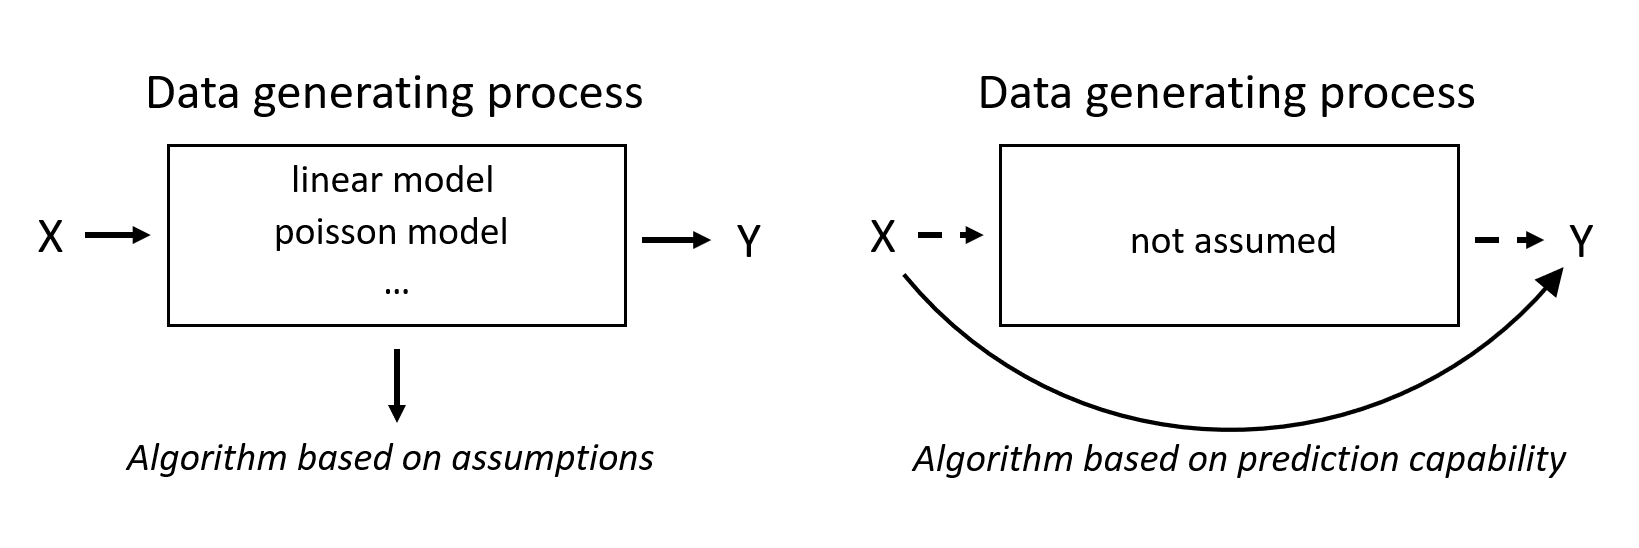
\includegraphics[width=0.9\textwidth]{figura24.png}
\caption{Differences between methods based on assumptions (left) and methods based on predictive capability (right).}
\label{figura24}
\end{figure}

\subsection{Regression and classification trees}
\label{decisiontrees}
Regression and classification trees, also known as decision trees are one of the simplest methods based on trees. They are based on a series of logical decisions structured in a flowchart form, with dichotomic decision nodes based on the different predictor variables. These nodes split into different branches of the tree depending on the decision. The initial node, also called the root node, is at the top of the tree. From there, data passes through various decision nodes until it reaches one of the final nodes of the tree, also called leafs, which contain the prediction of the model. \autoref{figura25} represents a classification tree for predicting relapse in breast cancer. One of the advantages of trees is their ease of interpretation. There is no need of formulas or difficult theory behind them. They are just a flowchart with dichotomic decisions at each node, so all the mechanisms by which a specific prediction is made are fully transparent even for non-experts. They also can deal naturally with categorical predictors and also with missing values and are virtually immune to outliers \parencite{venables2002tree} and to collinearity \parencite{loh2014fifty}. But, in spite of all these strengths, they also suffer from several issues which limit their usefulness when dealing with metabolomic data sets. One of the main issues is their non-smooth bias-variance curve. Small trees are usually too simple, thus underfiting the data (high bias), but they rapidly grow to very complex trees that overfit the data (high variance). This makes it very difficult to achieve a good balance between bias and variance resulting in a good predictive model. For this reason, single decision trees are only used for very simple problems, leaving the complex ones for more sophisticated tree-based methods.

\begin{figure}[hbtp]
\centering
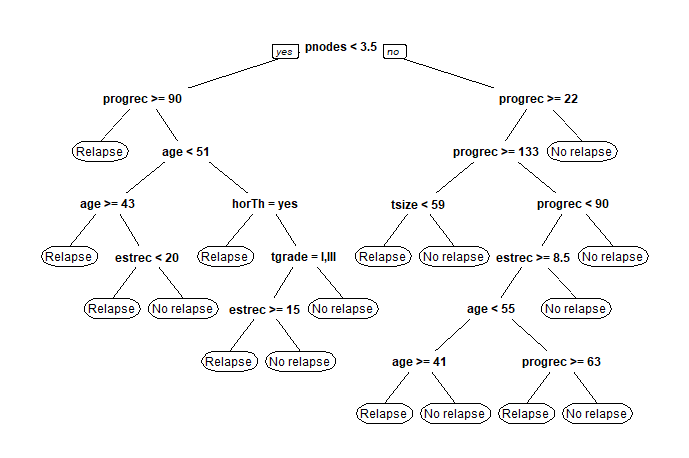
\includegraphics[width=0.9\textwidth]{figura25.png}
\caption{Classification tree for predicting relapse in breast cancer patients. Starting from the top one, each node tests a boolean condition which determines the direction of the next node to test until a terminal node is reached and a prediction is made.}
\label{figura25}
\end{figure}

\subsection{Random forests}
As explained in \autoref{decisiontrees}, single trees are not able to achieve a reasonable balance between bias and variance when adjusting the model. The method known as random forest \parencite{breiman2001random} is inspired in the reasoning behind what was already exposed in \autoref{figura20} of \autoref{penalmethods}. In that figure, there are two targets, the first one corresponding to a zero bias / high variance situation and the second one corresponding to a moderate bias / low variance situation. Since only one sample is usually available (corresponding to just one shot at the target), it is more reasonable to use the moderate bias / low variance target. However, if we had a sufficient amount of large enough samples and could fit one model to each sample, the zero bias / high variance situation would be the best, since averaging the different models would reduce variance and maintain the low bias. This is how random forest works. It creates different instances of the data set using bootstrap resampling \parencite{efron1994introduction} and trains one decision tree to each instance. Since bootstrap samples are correlated, predictor variables are selected at random at each node in each tree to make the models fitted to the different samples more diverse. When performing a prediction, the results of each tree are combined into a single outcome by voting. 

Random forests are among the best methods for predictive modelling, being immune to almost all of the problems commented for the other introduced methods and having very competitive error rates in almost all situations \parencite{fernandez2014we}. Their only drawbacks for its use when analyzing metabolomic data are that they are not easily interpretable and that they do not strictly provide variable selection, although they provide variable importance measures \parencite{archer2008empirical}.

\subsection{Boosting}
As random forest, boosting consists in combining different decision trees to improve prediction accuracy. But, instead of reducing variance like random forest, boosting combines small trees (or any other weak learner) to reduce bias \parencite{freund1996experiments}. The different resampled data sets are generated also differently. In the case of boosting, data sets are generated sequentially in an iterative way. \autoref{figura26} depicts a scheme of how boosting works.

\begin{figure}[hbtp]
\centering
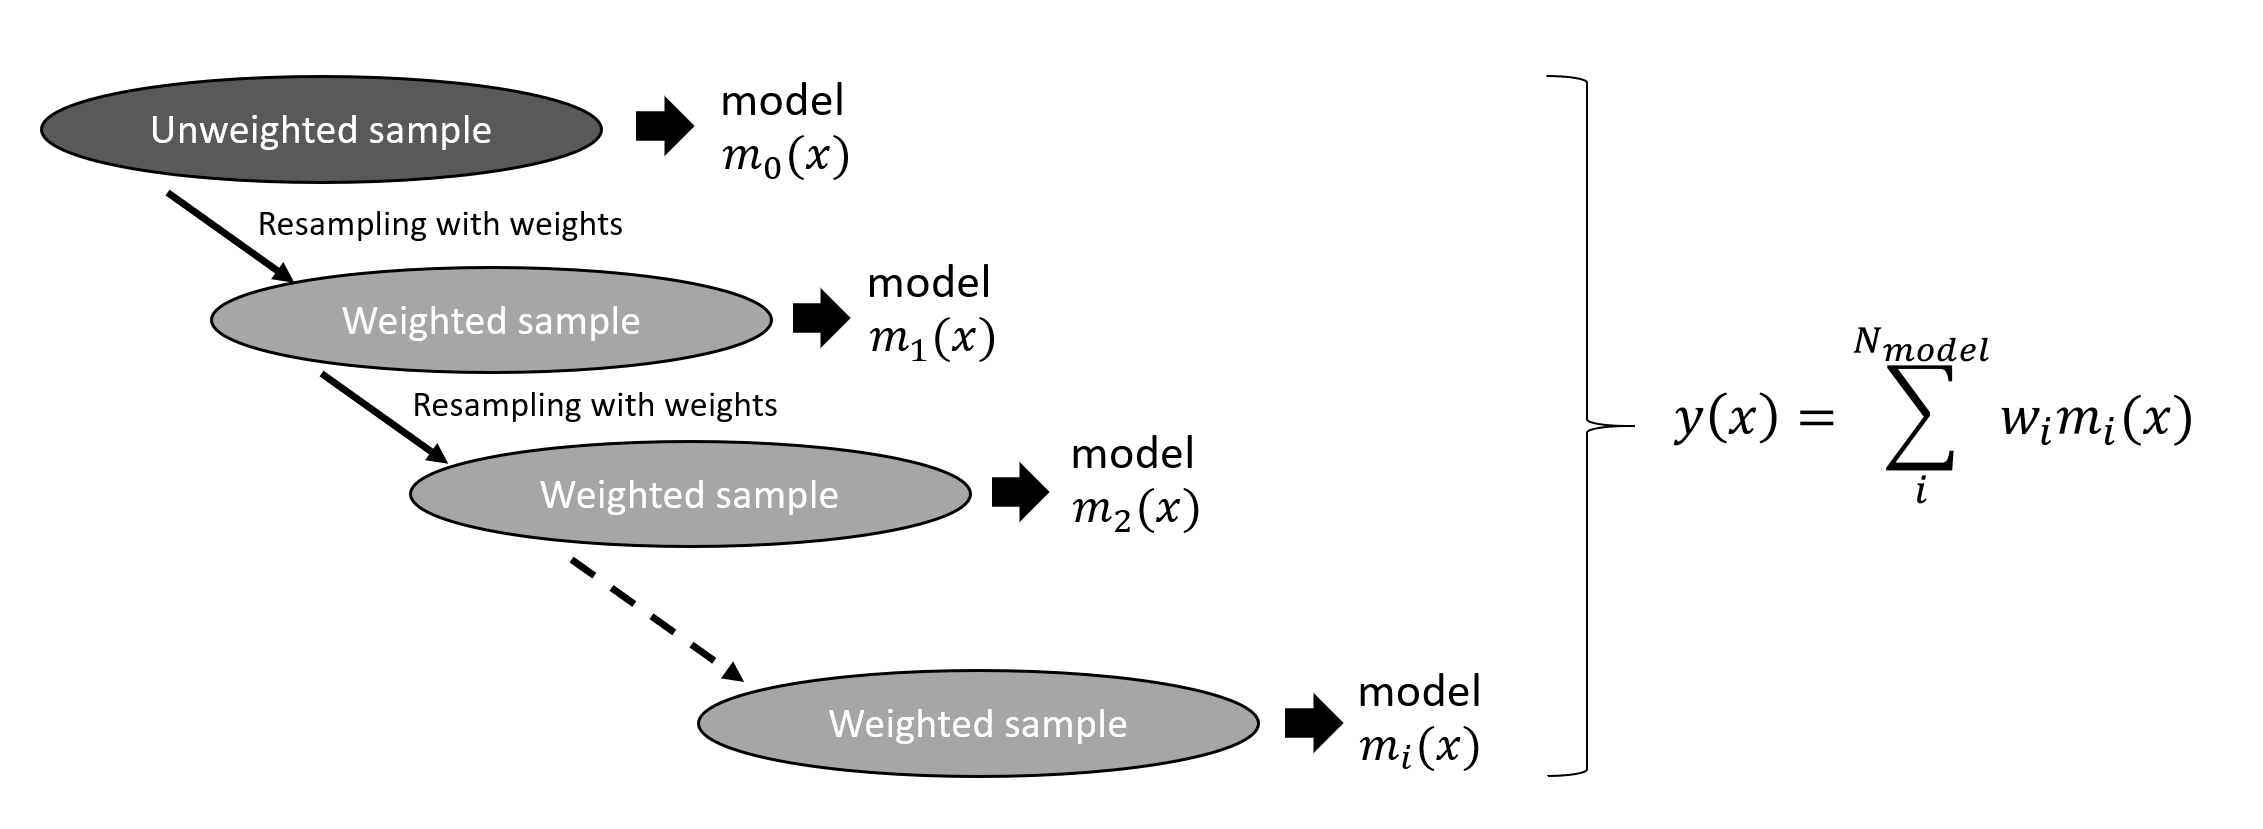
\includegraphics[width=0.85\textwidth]{figura26.png}
\caption{Representation of the boosting algorithm. Each time a model is fitted, a new weighted sample is generated based on the results of the model.}
\label{figura26}
\end{figure}

Beginning from an unweighted data set, the first tree is fitted and a new data set will be generated where observations that were mispredicted will appear more frequently than observations correctly predicted. This way, next model will learn from the mistakes of the previous one, improving prediction error. After this, a new data set will be produced where the mispredicted observations from the second model will be overrepresented compared to the correctly predicted observations. This steps will be repeated until the error rate is low enough. Predictions of the model are estimated using weighted voting based on their accuracy. As random forest, boosting is among the best methods for predictive modelling regarding prediction accuracy, but it suffers from the same issues as random forest regarding interpretability and variable selection \parencite{auret2011empirical}.

\section{Other methods}
Although projection, penalization and tree-based methods have been covered in detail, there are other methods worth mentioning when thinking about dealing with metabolomic data sets. Among them stand out neural networks \parencite{dayhoff2001artificial}, support vector machines \parencite{mahadevan2008analysis} and bayesian networks \parencite{bartel2013statistical}.

% ---------------------------------------------------------------------
% ---------------------------------------------------------------------
% ---------------------------------------------------------------------
\part{Materials and methods}

\chapter[Multiway data, methods for its analysis]{Multiway data, methods for its analysis}
\label{chapter:threeways}


% ---------------------------------------------------------------------
% ---------------------------------------------------------------------
\section{From 2D matrices to 3D arrays}
In most fields, data sets are usually represented by two dimensional matrices, where the rows are the observations and the columns are the different variables ($I \times J$). But in metabolomics, and in general in many other 'omic' sciences, sometimes these $I \times J$ data sets can be expanded by taking, for example, repeated measurements at different $K$ time points for each observation and producing a three-dimensional data structure ($I \times J \times K$) called three-way array (\autoref{figura27}) or, more generally, a multidimensional data structure called multi-way array \parencite{kroonenberg2016my}. Most of the modelling methods that have been explained in \autoref{chapter:modern_techniques} are not able of dealing with such data structures, which raise many methodological complications to the analyses. Therefore, different three-way or multi-way specific methods have been developed during the last decades to deal with this sort of data.

\begin{figure}[hbtp]
\centering
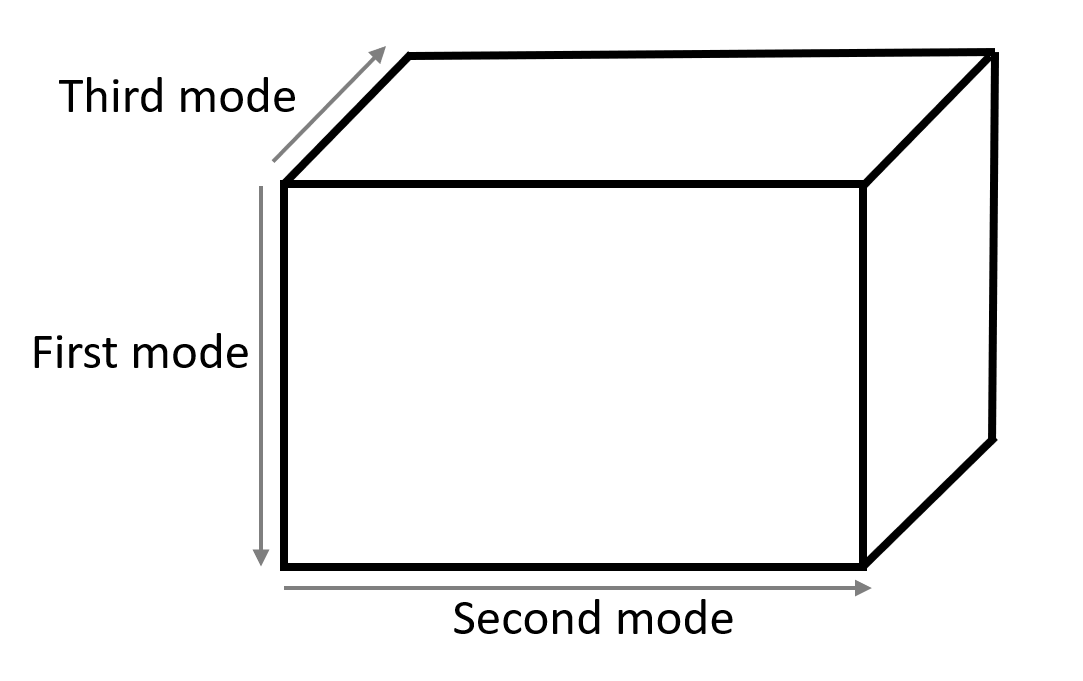
\includegraphics[width=0.60\textwidth]{figura27.png}
\caption{Representation of a three-way array.}
\label{figura27}
\end{figure}

\section{Exploration and description of N-way arrays}
\subsection{Unfolding}
One of the straightforward solutions for dealing with $N$-way arrays is performing an unfolding of the array into a two-dimensional matrix. This unfolding is performed by regrouping the elements of the higher order dimensions, also called modes, by extending the dimension of the second mode, as showed in \autoref{figura35}. After the unfolding, all statistical methods valid for two-dimensional matrices are applicable to the new structure, although the tridimensional structure of the data is lost, leading to a list of potential issues such as more complex models (too many parameters), loss of predictive power, loss of the multi-way information and greater difficulty in the interpretation of results.

\begin{figure}[hbtp]
\centering
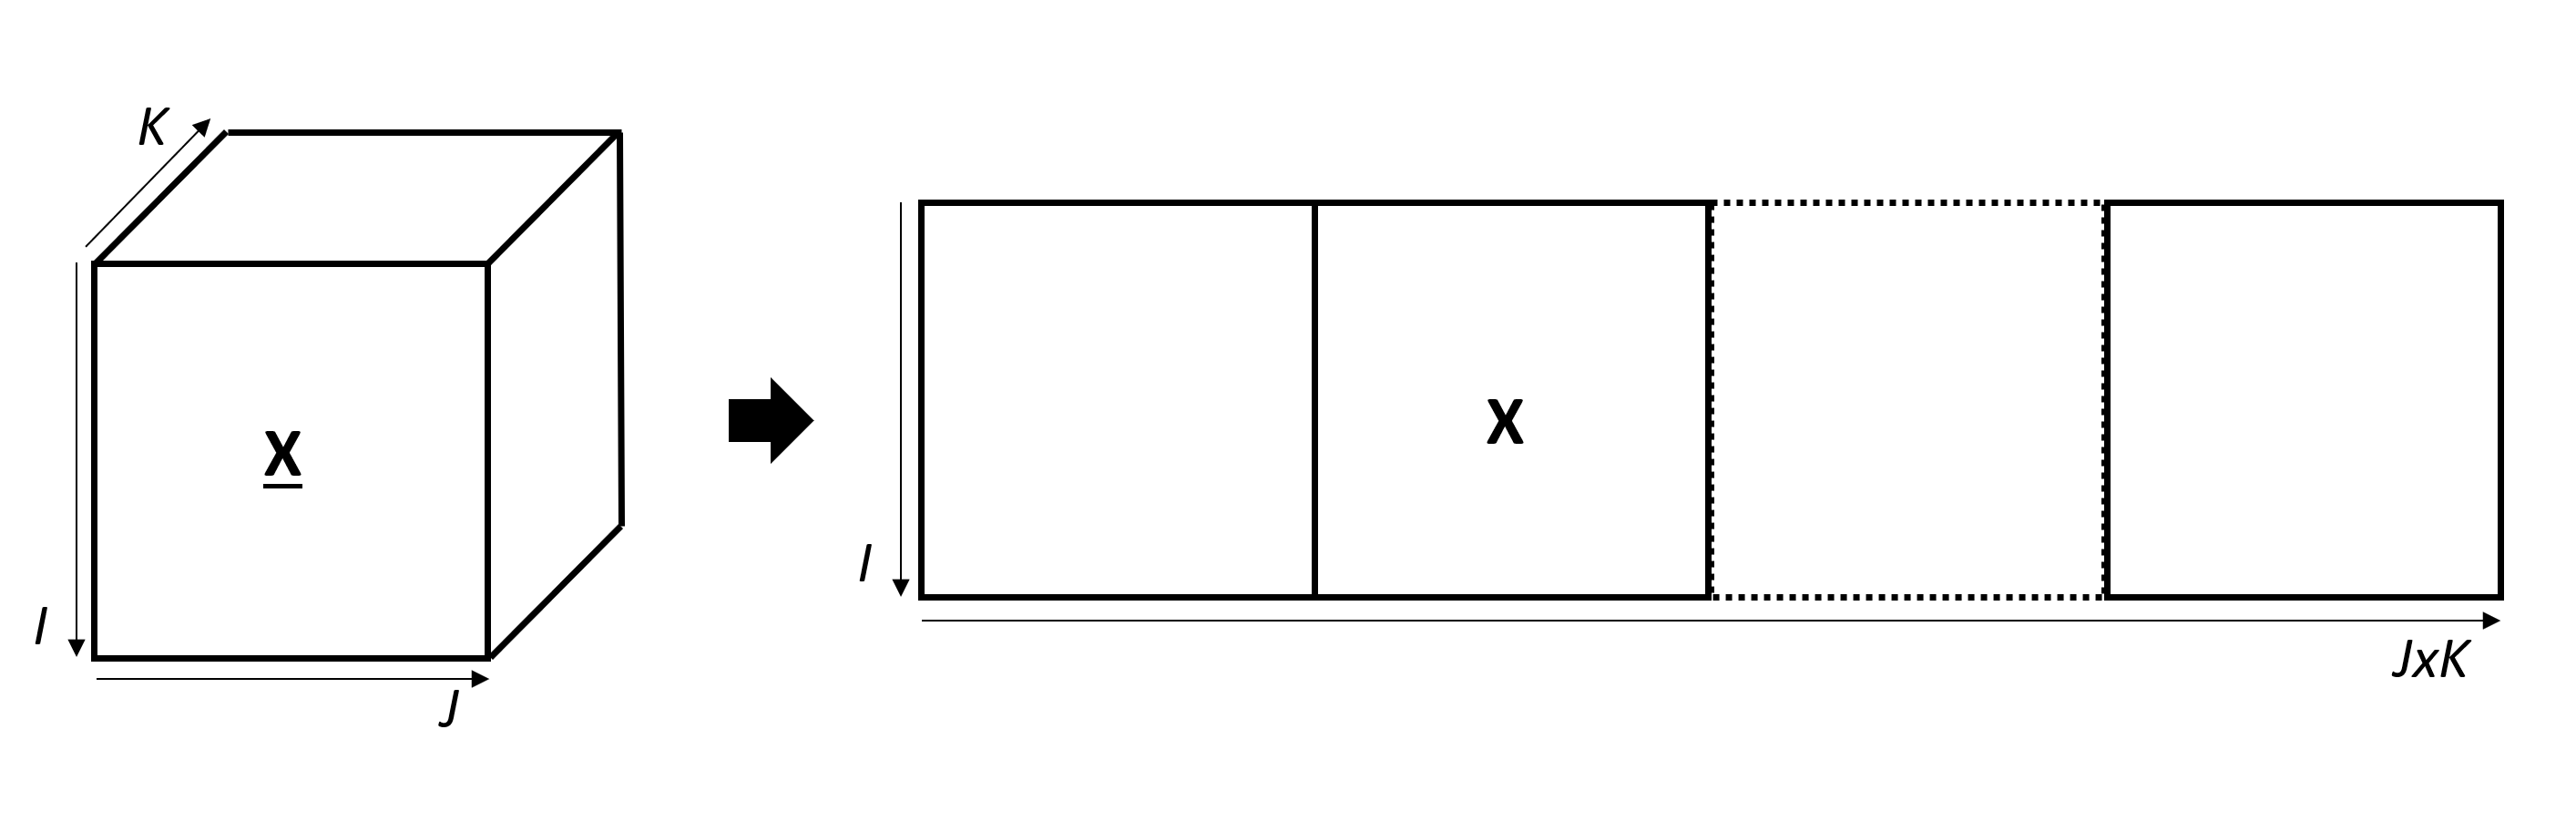
\includegraphics[width=0.95\textwidth]{figura35.png}
\caption[Unfolding of a three-way array into a two-dimensional matrix]{Unfolding of a three-way array ($I \times J \times K$) into a two-dimensional matrix ($I \times JK$).}
\label{figura35}
\end{figure}


\subsection{Tucker3}
When studying multi-way structures, the most general model that can be used is the Tucker3 model \parencite{tucker1966some}, also explained in detail by \textcite{kiers2001three}.

Assuming a three-way structure of the data, the Tucker3 model has the structure defined in \autoref{figura34}. This figure shows that the model is a weighted sum of all possible outer products, where the weights of the outer product between the $i$th factor from \textbf{A}, the $j$th factor from \textbf{B} and the $k$th factor from \textbf{C} is determined by element $g_{ijk}$ of the core. 

Model parameters are estimated by minimizing the squared sum of residuals $e_{lmn}$ as shown in \autoref{equation17}

\begin{equation}
x_{ijk}=\sum\limits_{l=1}^{w_1} \sum\limits_{m=1}^{w_2} \sum\limits_{n=1}^{w_3}a_{il}b_{jm}c_{kn}+e_{lmn}
\label{equation17}
\end{equation}

If the Kronecker product is used, defined as $\otimes$, unfolding the \textbf{\underline{X}} array, the \textbf{\underline{G}} core and the residuals \textbf{\underline{E}} into matrices \textbf{X}, \textbf{G} and \textbf{E} by fixing the first mode, the matrix expression of the model is as follows (\autoref{equation18}):

\begin{equation}
\textbf{\text{X}}=\textbf{\text{AG}}(\textbf{\text{C}}^T\otimes \textbf{\text{B}}^T)+\textbf{\text{E}}
\label{equation18}
\end{equation}

where \textbf{A} is the loadings matrix corresponding to the first mode, \textbf{G} is the matrix obtained after unfolding the \textbf{\underline{G}} core fixing the first mode, \textbf{B} and \textbf{C} are the loading matrices of the second and third mode respectively and \textbf{E} is the residuals matrix. The fact that the number of components is not forced to be the same in the different modes allows for the different loadings matrices to have different dimensions for each mode.

\begin{figure}[hbtp]
\centering
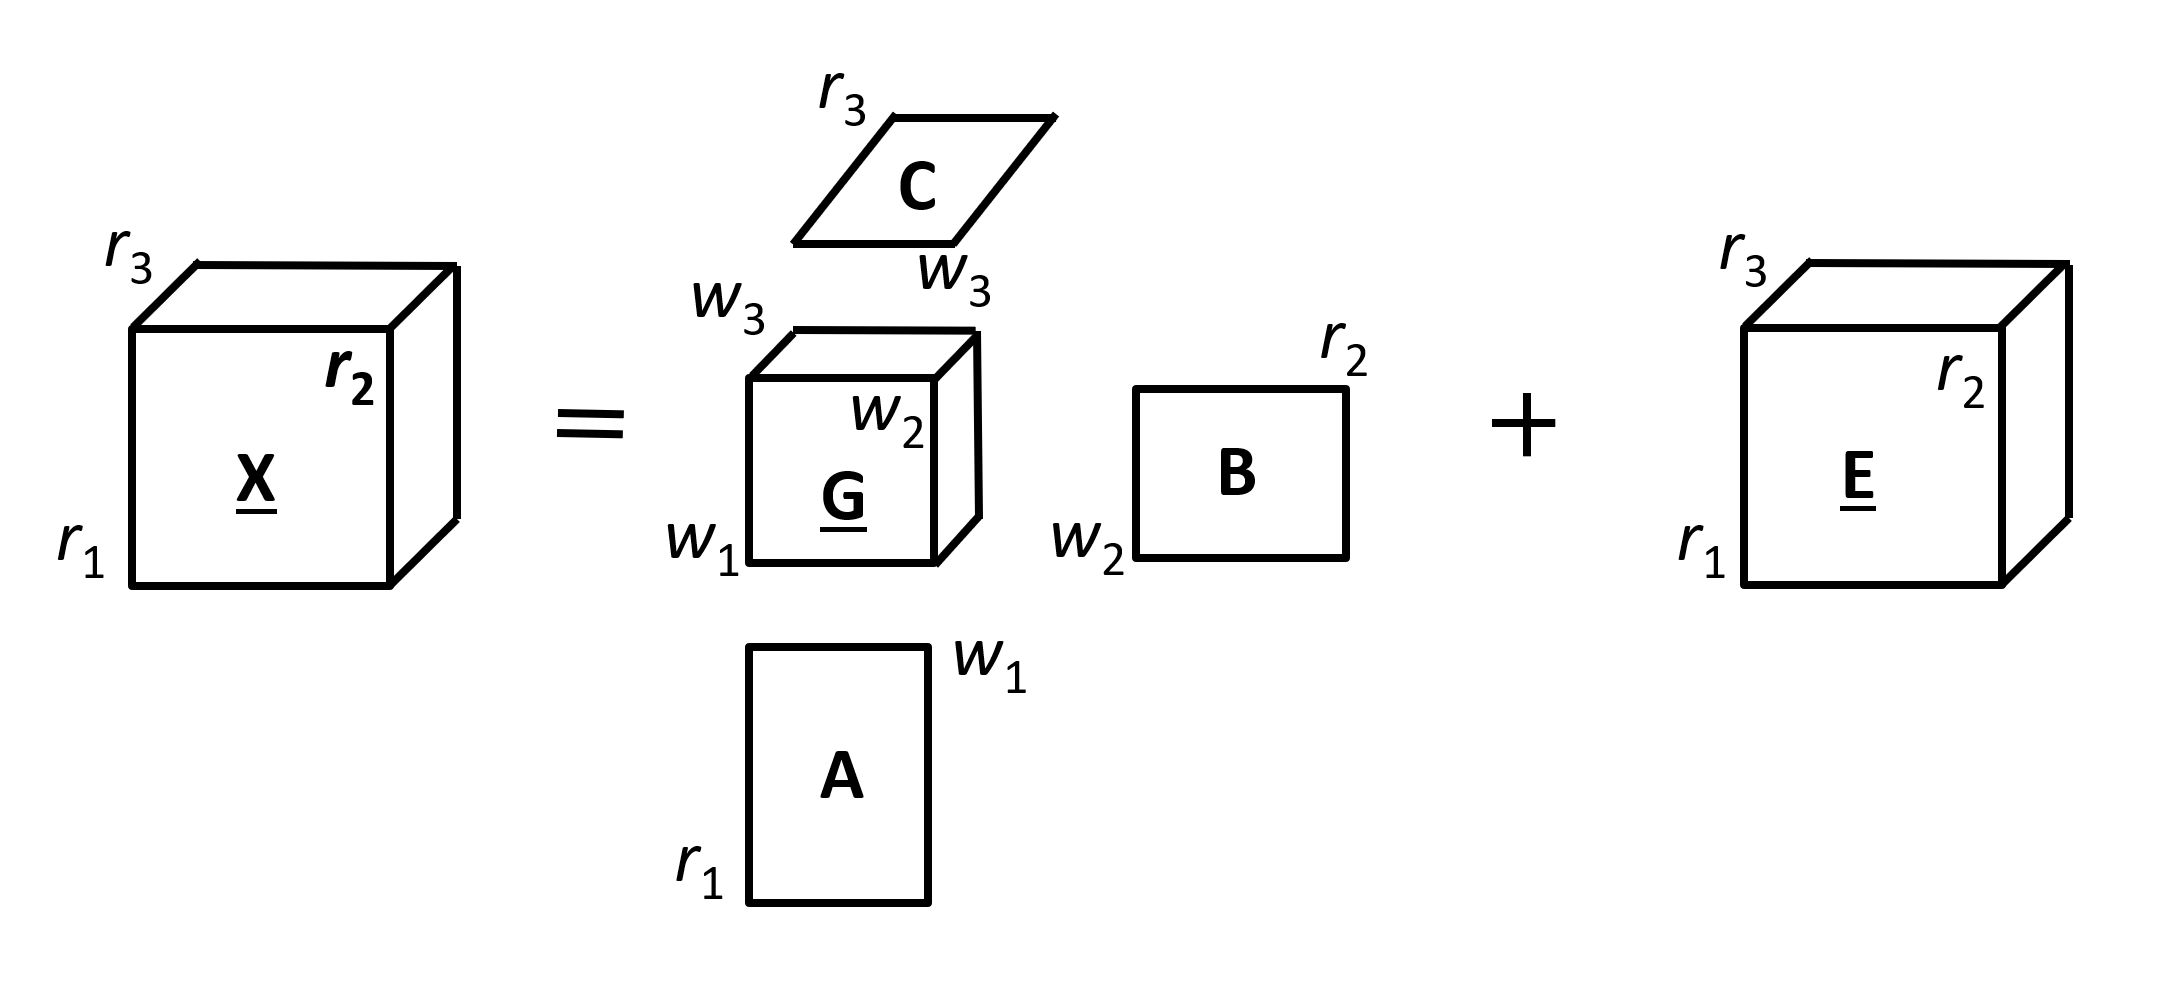
\includegraphics[width=0.85\textwidth]{figura34.png}
\caption[Scheme of the Tucker3 model]{Scheme of the Tucker3 model. The model consists on a weighted sum of outer products between the different factors stored in matrices \textbf{A}, \textbf{B} and \textbf{C}.}
\label{figura34}
\end{figure}

Of note, the compression performed by the model can be applied also to the first mode. This way, the \textbf{\underline{G}} core can be considered as an approximation to \textbf{\underline{X}}, which approximates the original array by the three matrices \textbf{A}, \textbf{B} and \textbf{C}.

It is important to take into account that the model has not a unique solution, because it has rotational freedom. In fact, the model can be so redundant that many elements of \textbf{\underline{G}} can be set to zero without altering the fit of the model, thus meaning they are associated to noise \parencite{montalban2005control}.

\subsection{PARAFAC}
The PARAFAC method is also a decomposition method for multi-way arrays. It can be derived from the Tucker 3 model by imposing superdiagonallity and identity in the structure of the \textbf{\underline{G}} core. Essentially, it is a generalization of PCA to three- or multi-way data structures \parencite{bro1997parafac}. The method was first developed by \textcite{harshman1970foundations} and \textcite{carroll1970analysis}, who named the method as CANDECOMP. In this method, the decomposition of the data is made into trilinear components, with each component consisting of one score vector and two loading vectors. The general structure of the PARAFAC model is presented in \autoref{figura36}.

\begin{figure}[hbtp]
\centering
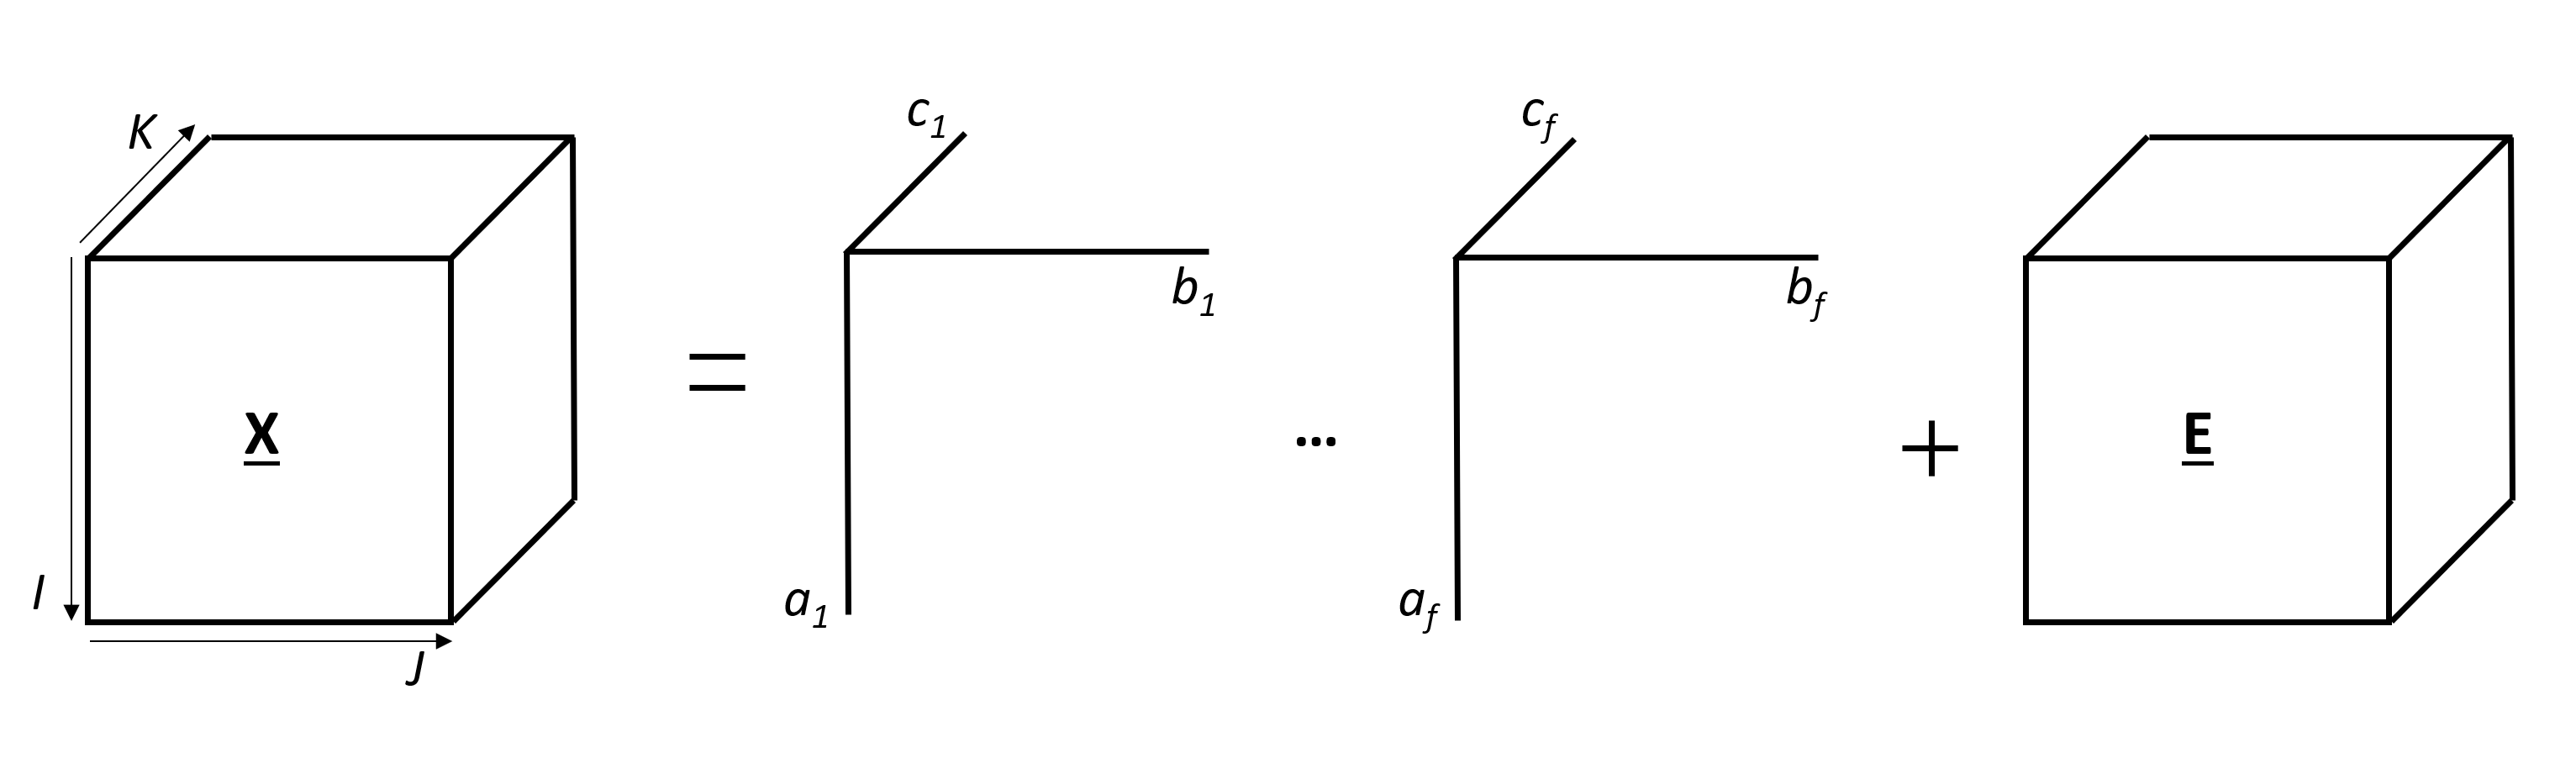
\includegraphics[width=0.9\textwidth]{figura36.png}
\caption{General structure of a PARAFAC model.}
\label{figura36}
\end{figure}

A PARAFAC model of a three-way array is given by three loading matrices, \textbf{A}, \textbf{B} and \textbf{C} with elements $a_{if}$, $b_{if}$ and $c_{kf}$. The model minimizes the sum of squares of residuals in \autoref{equation16}.

\begin{equation}
x_{ijk}=\sum\limits_{f=1}^F a_{ij}b_{jf}c_{kf}+e_{ijk}
\label{equation16}
\end{equation}

The matricial expression of the PARAFAC model can be obtained by Using the Khatri-Rao product \parencite{liu2008hadamard} and by unfolding the \textbf{\underline{X}} array into matrix \textbf{X} (\autoref{equation19}).

\begin{equation}
\textbf{\text{X}}=\textbf{\text{A}}(\textbf{\text{C}}|\otimes|\textbf{\text{B}})^T + \textbf{\text{E}} = \sum\limits_{f=1}^F a_f(c^T_f\otimes b^T_f)+\textbf{\text{E}}
\label{equation19}
\end{equation}

In the PARAFAC model, $a_f$, $b_f$ and $c_f$ are the $f$th columns of the loading matrices \textbf{A}, \textbf{B} and \textbf{C}, respectively.

The main advantage of PARAFAC over Tucker3 models is the impossibility of alternative solutions, that is, there is no posibility of rotation. This makes PARAFAC models more easily interpretable.

\section{Regression methods for \textit{N}-way arrays, \textit{N}-PLS}
\label{NPLSregression}
The $N$-PLS model is an extension of the standard PLS model to multi-way arrays based in the decomposition performed by the PARAFAC model \parencite{bro1996multiway}. Its aim is studying relationships between some three-way (or N-way) \textbf{\underline{X}} (e.g. $I \times J \times K$) data structure and any \textbf{\underline{Y}} (e.g. $I \times L \times M$) data structure by maximizing the covariance between \textbf{\underline{X}} and \textbf{\underline{Y}} data arrays. For achieving this, a multilinear model is fitted simultaneously to the \textbf{\underline{X}} and the \textbf{\underline{Y}} arrays with a regression model relating them together. The structure of the $N$-PLS model is presented in \autoref{figura38}.

\begin{figure}[hbtp]
\centering
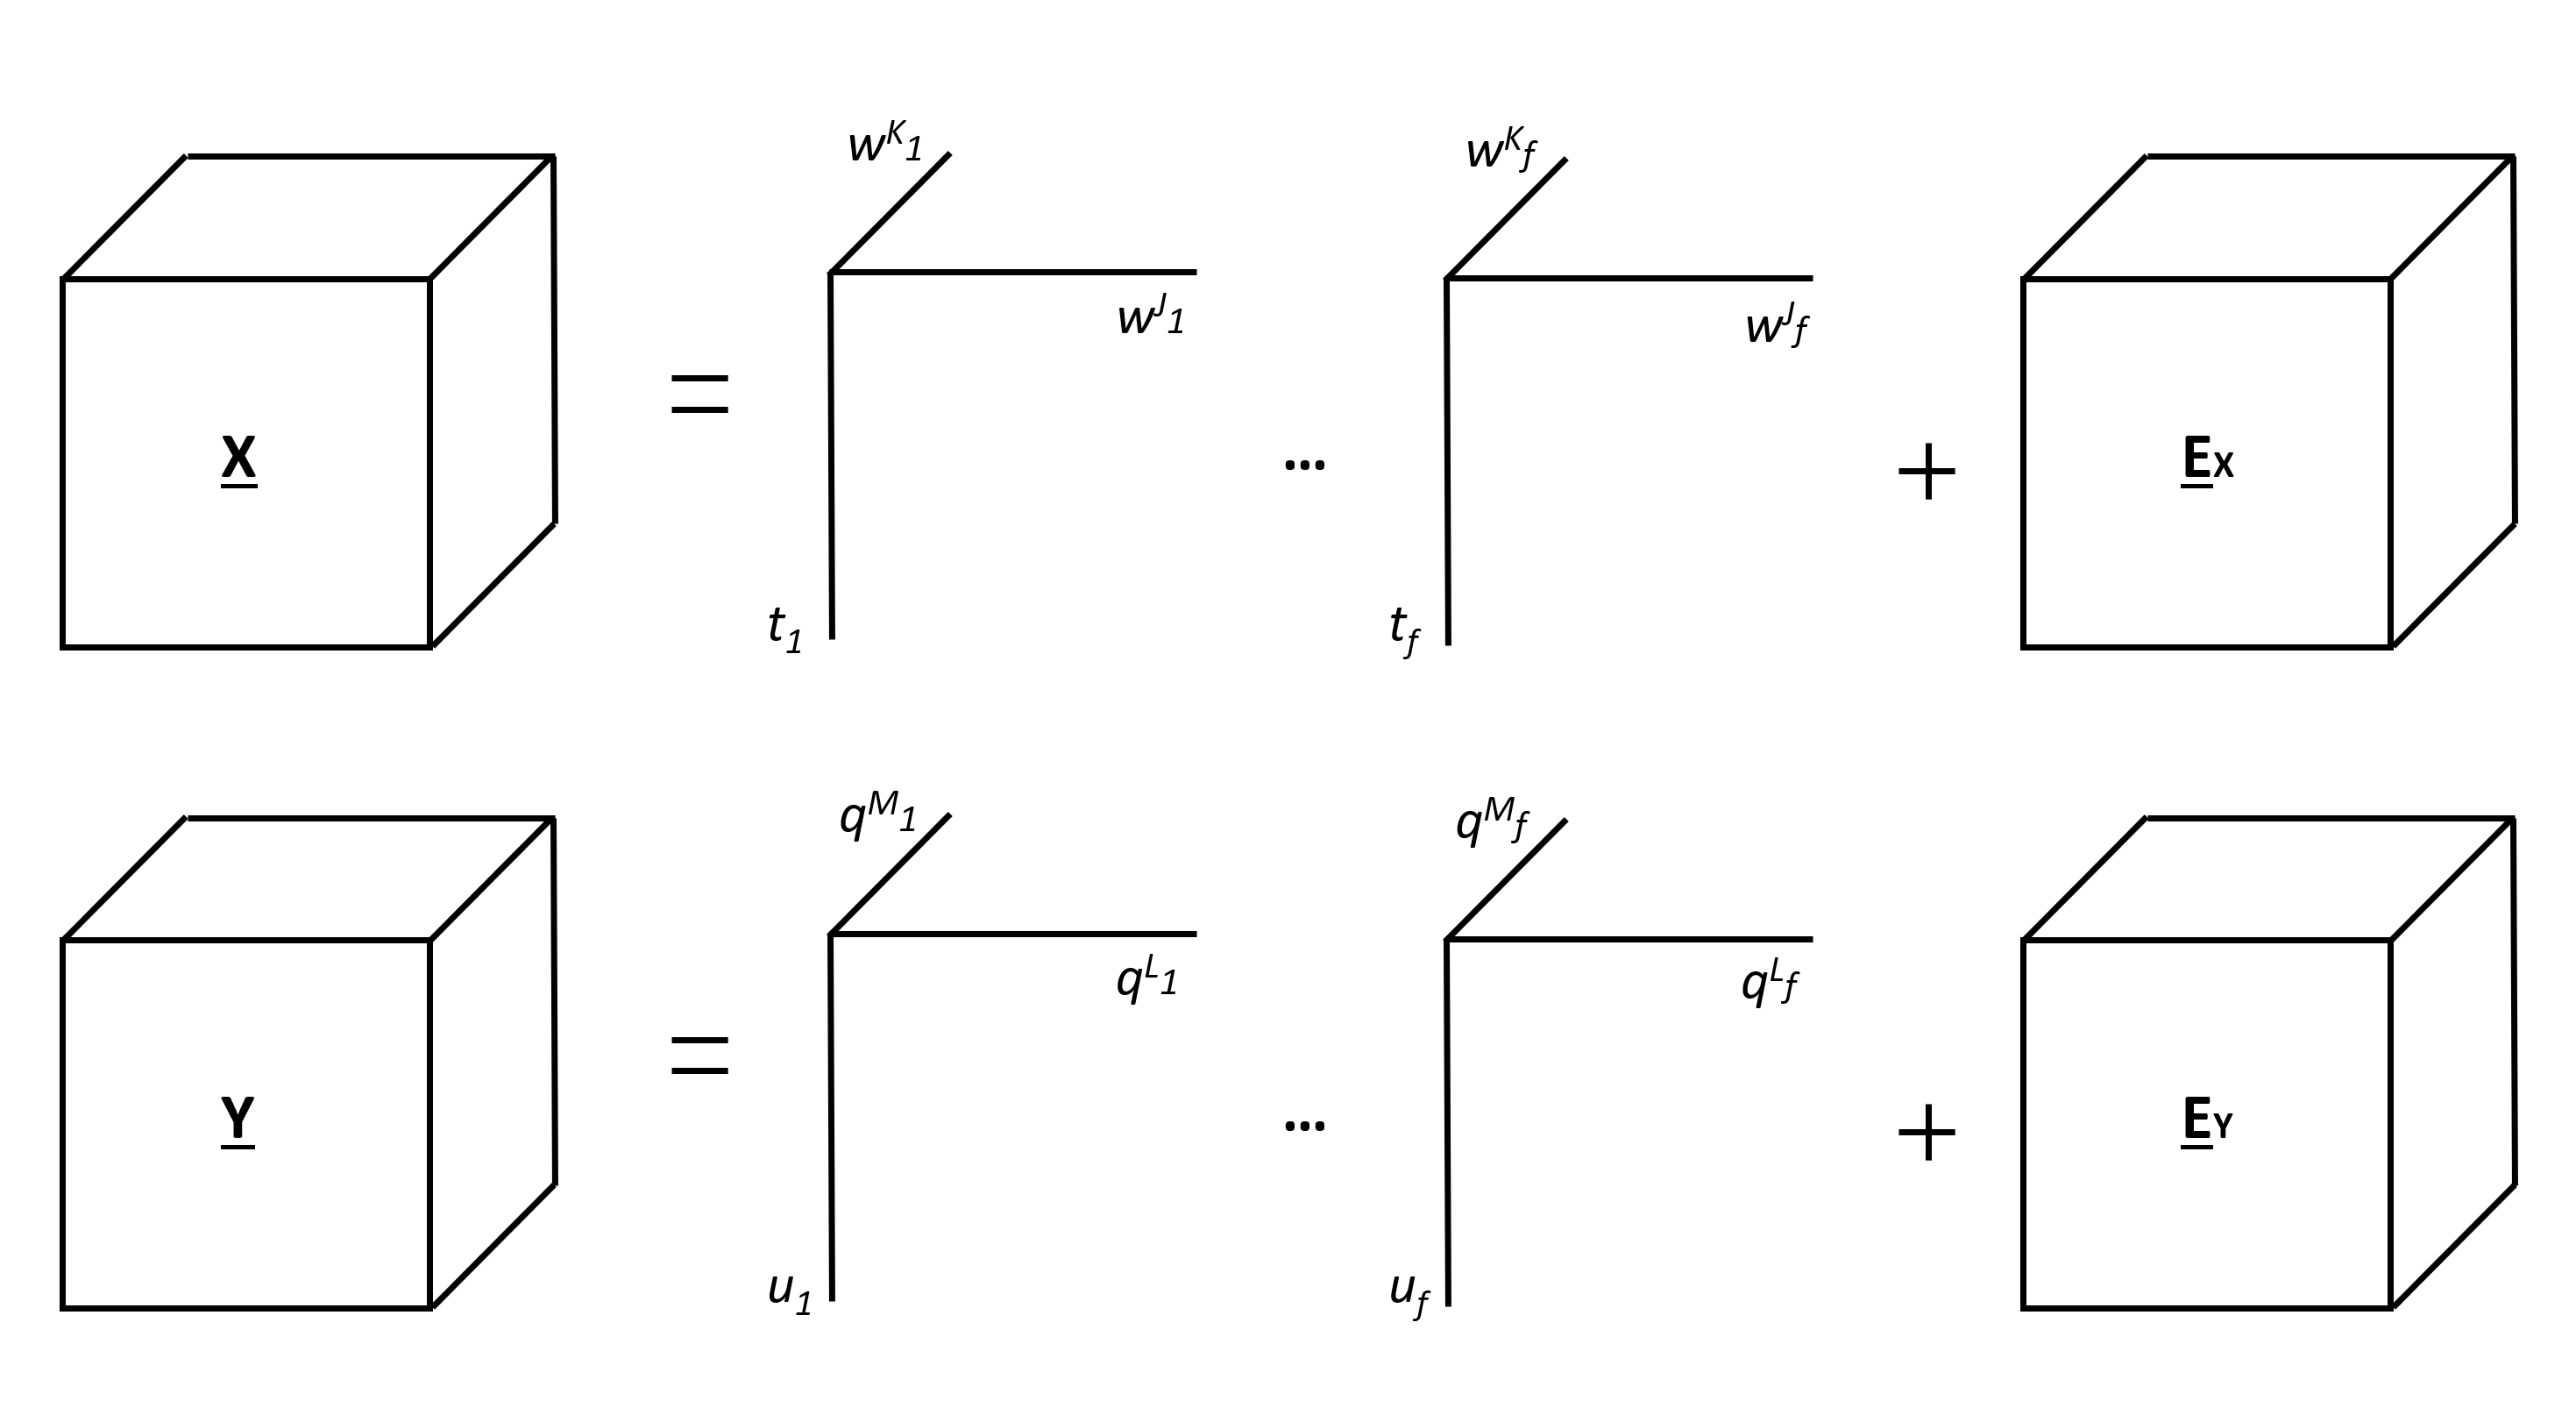
\includegraphics[width=0.85\textwidth]{figura38.png}
\caption{General structure of a $N$-PLS model.}
\label{figura38}
\end{figure}


Considering \textbf{X} ($I \times JK$) the unfolded version of \textbf{\underline{X}}, \textit{N}-PLS tries to find latent spaces $\textbf{\text{W}}^{J}$ and $\textbf{\text{W}}^{K}$ that maximize the covariance between \textbf{X} and \textbf{Y}, so it can be expressed as:

\begin{equation}
\textbf{\text{X}}=\textbf{\text{T}}(\textbf{\text{W}}^{K}|\otimes{}|\textbf{\text{W}}^{J})^{T}+\textbf{\text{R}}
\label{equation01}
\end{equation}

Afterwards decomposing \textbf{\underline{X}} from \textbf{X} using the improved $N$-PLS version expression \parencite{bro2001difference}, in order to obtain residuals with better statistical properties:

\begin{equation}
\textbf{\text{X}}=\textbf{\text{T}}\textbf{\text{Gu}}(\textbf{\text{W}}^{K}\otimes{}\textbf{\text{W}}^{J})^{T}+\textbf{\text{R}}^{\boldsymbol{\prime{}}}
\label{equation02}
\end{equation}

In the same way, \textbf{\underline{Y}} can be decomposed by unfolding \textbf{\underline{Y}} ($I \times L \times M$) into \textbf{Y} ($I \times LM$) as:

\begin{equation}
\textbf{\text{Y}}=\textbf{\text{U}}(\textbf{\text{Q}}^{M}|\otimes{}|\textbf{\text{Q}}^{L})^{T}+\textbf{\text{R}}^{\boldsymbol{\prime{}\prime{}}}
\label{equation03}
\end{equation}

In this case, $\textbf{\text{W}}^{K}$ and $\textbf{\text{W}}^{J}$ refer to the weights of the third and of the second mode, respectively; whereas $\textbf{\text{T}}$ matrix gathers the scores of the samples at each component extracted, in the first mode. $|\otimes{}|$ is the Khatri-Rao product and $\otimes{}$ the Kronecker product, which forbid or allow (respectively) to take interactions between the different modes components into account. 
\textbf{Gu} is the core array (unfolded) of a Tucker3 decomposition when using \textbf{T}, $\textbf{\text{W}}^{K}$ and $\textbf{\text{W}}^{J}$ as loadings, in order to obtain a better (or at least not worse) approximation of the \textbf{\underline{X}} array \parencite{smilde2005multi}. Finally, $\textbf{\text{R}}^{\boldsymbol{\prime{}}}$ incorporates the residuals. Analogously, \textbf{U} refers to the \textbf{Y} scores, and $\textbf{\text{Q}}^{M}$ and $\textbf{\text{Q}}^{L}$ to the loadings of the array \textbf{\underline{Y}}.
Finally, from the scores \textbf{T} and \textbf{U}, as well from the \textbf{W} weights, a $\textbf{\text{B}}_{PLS}$ regression matrix can be obtained \parencite{bro1998multi} so

\begin{equation}
\textbf{\text{Y}}=\textbf{\text{X}}\textbf{\text{B}}_{PLS}+\textbf{\text{R}}^{\boldsymbol{\prime{}\prime{}\prime{}}}
\label{equation04}
\end{equation}

In summary, $N$-PLS allows for the application of the well known standard PLS model to multi-way arrays, being able to exploit the multidimensional structure of the data, reducing the inclusion of noise, and producing more parsimonious models than standard PLS models applied to unfolded matrices. 


\section{Software for analyzing three-way data}
\subsection{\texttt{R} programming language}
\texttt{R} \parencite{ihaka1996r, rsoftware} is a programming language designed for statistical programming, derived from the \texttt{S} language, which was developed in the Bell Laboratories by Rick Becker, John Chambers and Allan Wilks in the 60s. It is free software and open source, and was designed specifically for performing data analysis and statistical tasks. Since it is open source, \texttt{R} has thousands of developers, which results in more than 10000 packages in the main software repository for \texttt{R} named \textit{CRAN} (\autoref{figura13}) and more than 1300 packages in the \textit{Bioconductor} repository, specialized in packages for the analysis of 'omic' data. For this reasons, \texttt{R} has become a standard for data analysis in many scientific fields such as physics, biology and medicine among others \parencite{goztepe4facto}. 

\begin{figure}[hbtp]
	\centering
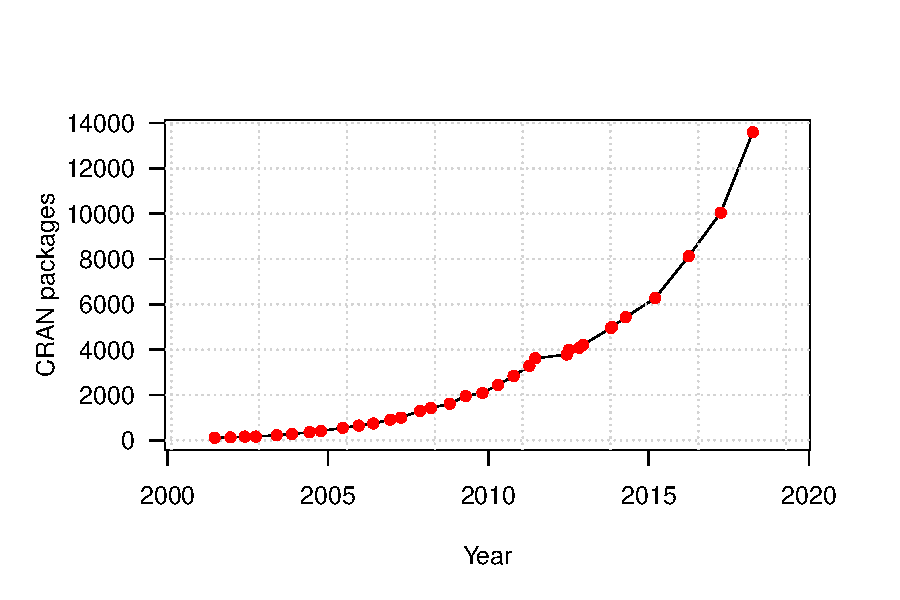
\includegraphics[width=0.7\textwidth]{figura13.pdf}
\caption[Number of R packages on CRAN since 2002]{Number of R packages on CRAN has been growing at an exponential rate since 2002.}
\label{figura13}
\end{figure}

With the huge number of packages at the disposal of \texttt{R} users, many advanced functions have already been programmed and are available for their use or reuse when programming new functionalities. Apart from the main repository (CRAN) there are other important repositories with thousands of packages more such as \textit{R-Forge}, \textit{Bioconductor} or even \textit{Github}. All this functionallity and the fact that R is open source motivated the election of \texttt{R} as the language for developing all the techniques and tools presented in this thesis.

\subsection{\texttt{R} packages for the analysis of three-way data}
Most three-way data procedures are implemented in MATLAB\textsuperscript{\tiny\textregistered} \textcite{MATLAB:2010} (or previous versions of the software). Concretely, the $N$-way toolbox by \textcite{andersson2000n} provides a comprehensive set of functions for dealing with three- and multi-way arrays in MATLAB\textsuperscript{\tiny\textregistered}. \texttt{R}, on the other hand, only has two packages dedicated to the analysis of three- or multi-way data. The packages \texttt{PTAk} \parencite{leibovici2010spatio} and \texttt{ThreeWay} \parencite{giordani2014three}, offer a suit of functions for handling three-way arrays in \texttt{R}. These functions include Tucker3 and PARAFAC models and also some processing methods for three-way data such as centering, scaling, unfolding and normalizing arrays. However, $N$-PLS is notably missing from these packages, so no prediction method for three-way arrays was implemented in \texttt{R} before the release of the \texttt{sNPLS} package developed in this thesis. In this way, with the development of the package, it has not only been implemented a newly developed method such as sparse $N$-PLS, but also enabled the use of standard $N$-PLS regression models to \texttt{R} users.

% ---------------------------------------------------------------------
% ---------------------------------------------------------------------
% ---------------------------------------------------------------------
\part{Results}
\chapter[Sparse \textit{N}-PLS, a method for variable selection in multiway data sets]{Sparse \textit{N}-PLS, a method for variable selection in multiway data sets}



% ---------------------------------------------------------------------
% ---------------------------------------------------------------------
\section{Sparse \textit{N}-PLS, integration of L1 penalization in the \textit{N}-PLS algorithm}
\label{NPLSpenalization}
As commented in the previous chapter, it is proposed to introduce the L1-penalization in the $N$-PLS algorithm. Since there are three modes, the aim is to perform selection not only on the second mode (variables), but also on the third mode. To this aim, a similar approach to that of \cite{le2008sparse} is used. Briefly, to achieve sparse versions of $\textbf{\text{w}}^\text{J}$ and $\textbf{\text{w}}^\text{K}$ for each latent variable, the soft-thresholding penalty function $\beta_j^{lasso}=sgn(\beta_j^{LS})(|\beta_j^{LS}|-\lambda)^+$ is introduced in the $N$-PLS algorithm right after the SVD at the $\textbf{\text{w}}^\text{J}$ and $\textbf{\text{w}}^\text{K}$ determination. The complete algorithm is as follows \autoref{figura40}:


\vspace{20pt}
Center \textbf{\underline{X}} and \textbf{\underline{Y}}, and unfold \textbf{\underline{X}} (and \textbf{\underline{Y}} when necessary) into a two-way matrix.

Let \textbf{u} be some column of \textbf{Y}, and set \textit{f}=1

\begin{enumerate}
    \item $\textbf{\text{w}}^\text{T}=\textbf{\text{u}}^\text{T}\textbf{\text{X}}/\textbf{\text{u}}^\text{T}\textbf{\text{u}}$
    \item Build \textbf{Z} by refolding \textbf{w} according to the modes dimensions
    \item Determine $\textbf{\text{w}}^\text{J}$ and $\textbf{\text{w}}^\text{K}$ by SVD
    \item L1-penalization inclusion
    \begin{enumerate}
        \item Apply soft-thresholding on $\textbf{\text{w}}^\text{J}$: $\beta_j^{lasso}=sgn(\beta_j^{LS})(|\beta_j^{LS}|-\lambda)^+$ 
        \item Apply soft-thresholding on $\textbf{\text{w}}^\text{K}$: $\beta_j^{lasso}=sgn(\beta_j^{LS})(|\beta_j^{LS}|-\lambda)^+$ 
        \item Input the new \textbf{w} as kronecker($\textbf{\text{w}}^\text{K}, \textbf{\text{w}}^\text{J}$)
    \end{enumerate}
    \item $\textbf{\text{t}}=\textbf{\text{Xw}}/\textbf{\text{w}}^\text{T}\textbf{\text{w}}$
    \item $\textbf{\text{q}}=\textbf{\text{Y}}^\text{T}\textbf{\text{t}}/\text{norm}(\textbf{\text{Y}}^\text{T}\textbf{\text{t}})$
    \item $\textbf{u}=\textbf{Yq}$
    \item Check for convergence. If it is achieved, continue; otherwise, go to 1
    \item $\textbf{\text{b}} = (\textbf{\text{T}}^\text{T}\textbf{\text{T}})^{-1}\textbf{\text{T}}^\text{T}\textbf{\text{u}} \text{; where} \ \textbf{\text{T}}=[\text{t1}\ \text{t2} \text{…} \text{t}_f]$
    \item $\textbf{\text{X}} = \textbf{\text{X}}-\textbf{\text{tw}}^\text{T} \ \text{and} \ \textbf{\text{Y}} = \textbf{\text{Y}}-\textbf{\text{tbq}}^\text{T}$
    \item \textit{f} = \textit{f}+1. Continue from step 1 until a good description of \textbf{Y}
\end{enumerate}
\vspace{20pt}

This algorithm is applicable to both the standard regression (continuous response) and the discriminant version of the $N$-PLS model, i.e. $N$-PLS-DA. In the case of $N$-PLS-DA, \textbf{\underline{Y}} is a \textbf{y} vector formed by ones and zeros, each of the two values related to one of the two classes to be segregated. 

\begin{figure}[hbtp]
\centering
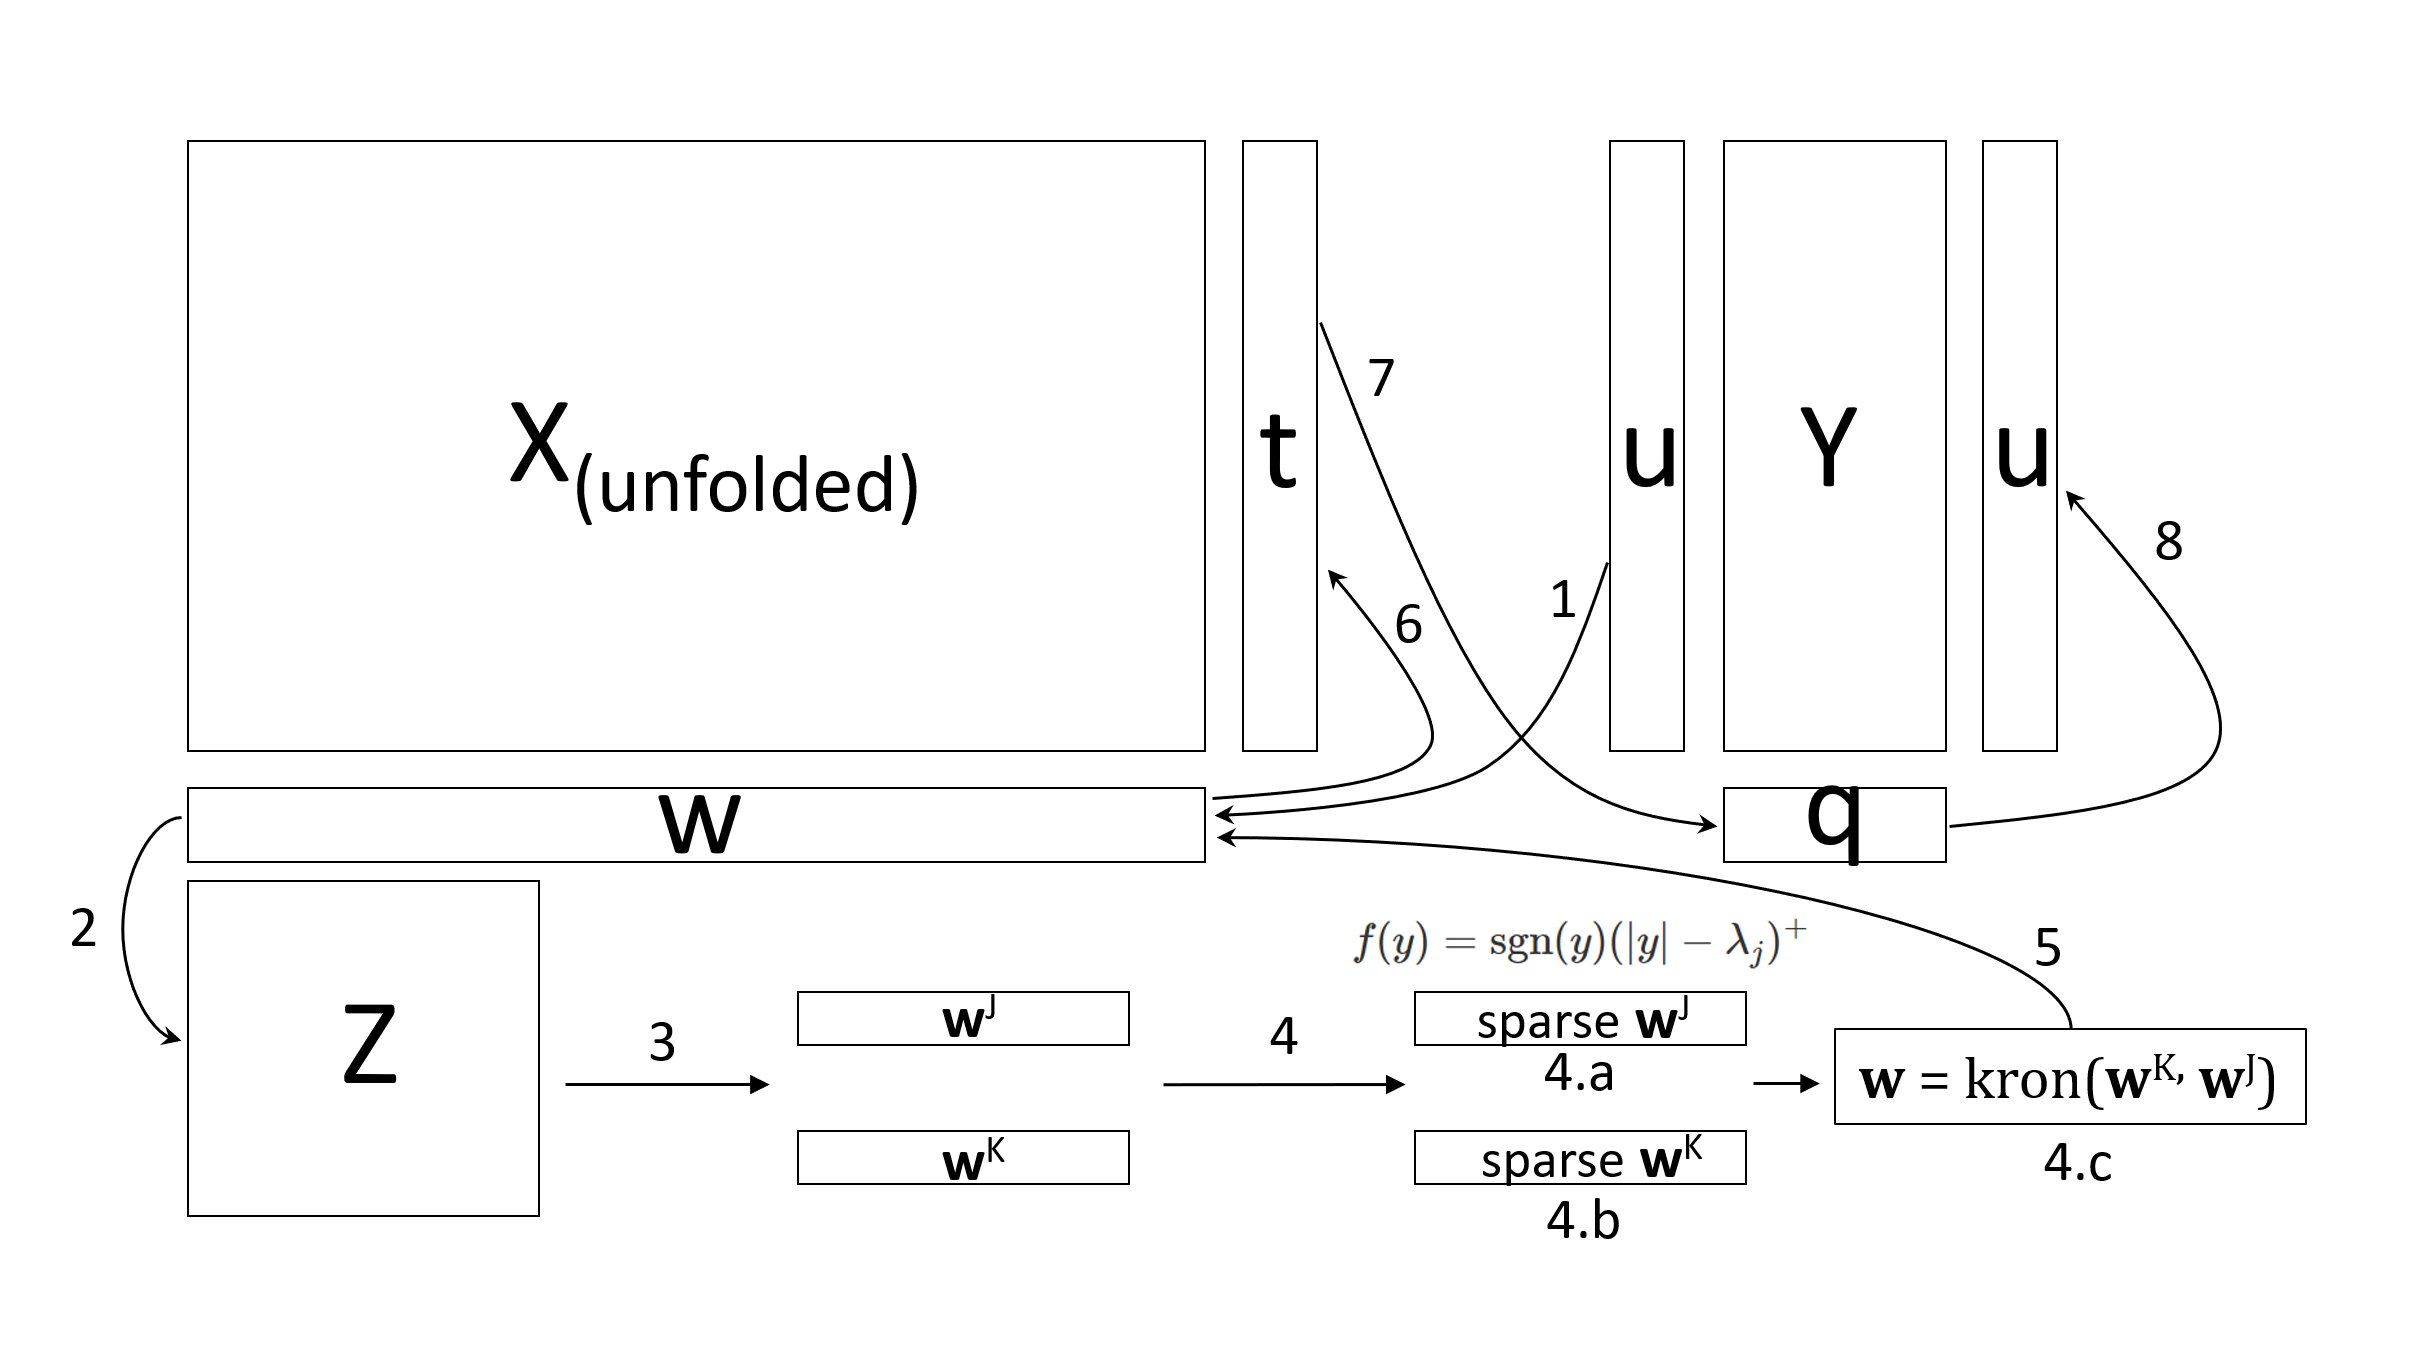
\includegraphics[width=1\textwidth]{figura40.png}
\caption[Scheme detailing the different steps of the sNPLS algorithm]{Scheme detailing the different steps of the sNPLS algorithm as explained in the previous page. \vspace{15pt}}
\label{figura40}
\end{figure}



\section{Hyperparameters of the sparse \textit{N}-PLS algorithm}
\label{hyperparameters}
Hyperparameters are tuneable parameters of the model, whose values are specified before starting the algorithm instead of determined inside the algorithm as standard parameters. L1-penalization has one hyperparameter, called the penalization factor (the amount of L1-penalization to apply). However, since the L1-penalization is applied to both $\textbf{\text{w}}^\text{J}$ and $\textbf{\text{w}}^\text{K}$ the number of hyperparameters for a sparse $N$-PLS model (sNPLS) is three: the number of components (shared with the standard $N$-PLS model), the number of variables to select at each component, and the number of elements of the third mode to select at each component. The number of components can range between one and $J$, and the number of variables per component or elements of the third mode per component can range between zero and $J$ and zero and $K$, respectively. It is necessary that at least one component includes one selected variable and one element of the third mode to fit a valid model. A sparse $N$-PLS model where all variables and all elements of the third mode are forced to be selected reduces to a general $N$-PLS model, where only the number of components acts as hyperparameter.

\subsection{Tuning of the parameters}
Optimization of the hyperparameter values is necessary to achieve optimal prediction power or optimal variable selection performance in the case of sNPLS. One important point to take into account is that consistency (selecting the right variables) and minimizing prediction error appear to be non-compatible \parencite{yang2005can}, so the tuning criterion has to be adapted depending on the main objective of the analysis. For the objective of variable selection, \textcite{zou2005regularization} mention the option of just choosing the desired number of non-zero coefficients as a viable alternative for interpretation purposes. In the present approach, the focus is set on minimizing prediction error, so to perform this tuning of the parameters, a grid search of the hyperparameter space \parencite{lameski2015svm} is proposed guided by the mean squared prediction error evaluated by cross-validation \parencite{duarte2017empirical}. More specifically, the approach consists on performing $K$-fold cross-validation repeatedly and averaging their results, to alleviate instability in the selection of parameters because of high variance in the single cross-validation results \parencite{krstajic2014cross}. This high variance entails that different runs of the cross-validation procedure can yield different results regarding the estimated best set of the parameters and also that the estimation of the best set of parameters is prone to overfitting (bias-variance tradeoff).

Briefly, K-fold cross-validation consists on randomly splitting the data set in a number of folds, $K$, and perform $K$ iterations of model fitting and testing, where a different fold is used as test set in each iteration while the other folds are used to train the model. This way, an out-of-sample estimate for the prediction error of the model is estimated at each iteration. Later, all estimates are averaged to get the mean cross-validated error. 

The procedure is performed as follows:
\vspace{20pt}
\begin{enumerate}
    \item Divide the data set in K subsets (ideally of equal size)
    \item For each k in 1, \dots K:
    \begin{itemize}
        \item Train the model on $(x_i, y_i)$ where $i \notin F_k$
        \item Estimate prediction error on $(x_k, y_k)$ as $E_k$
    \end{itemize}
    \item Average all errors to get the $CVE$ estimate
\end{enumerate}

\vspace{20pt}
A scheme of the procedure for K-fold cross-validation is represented in \autoref{figura39}.

\begin{figure}[hbtp]
\centering
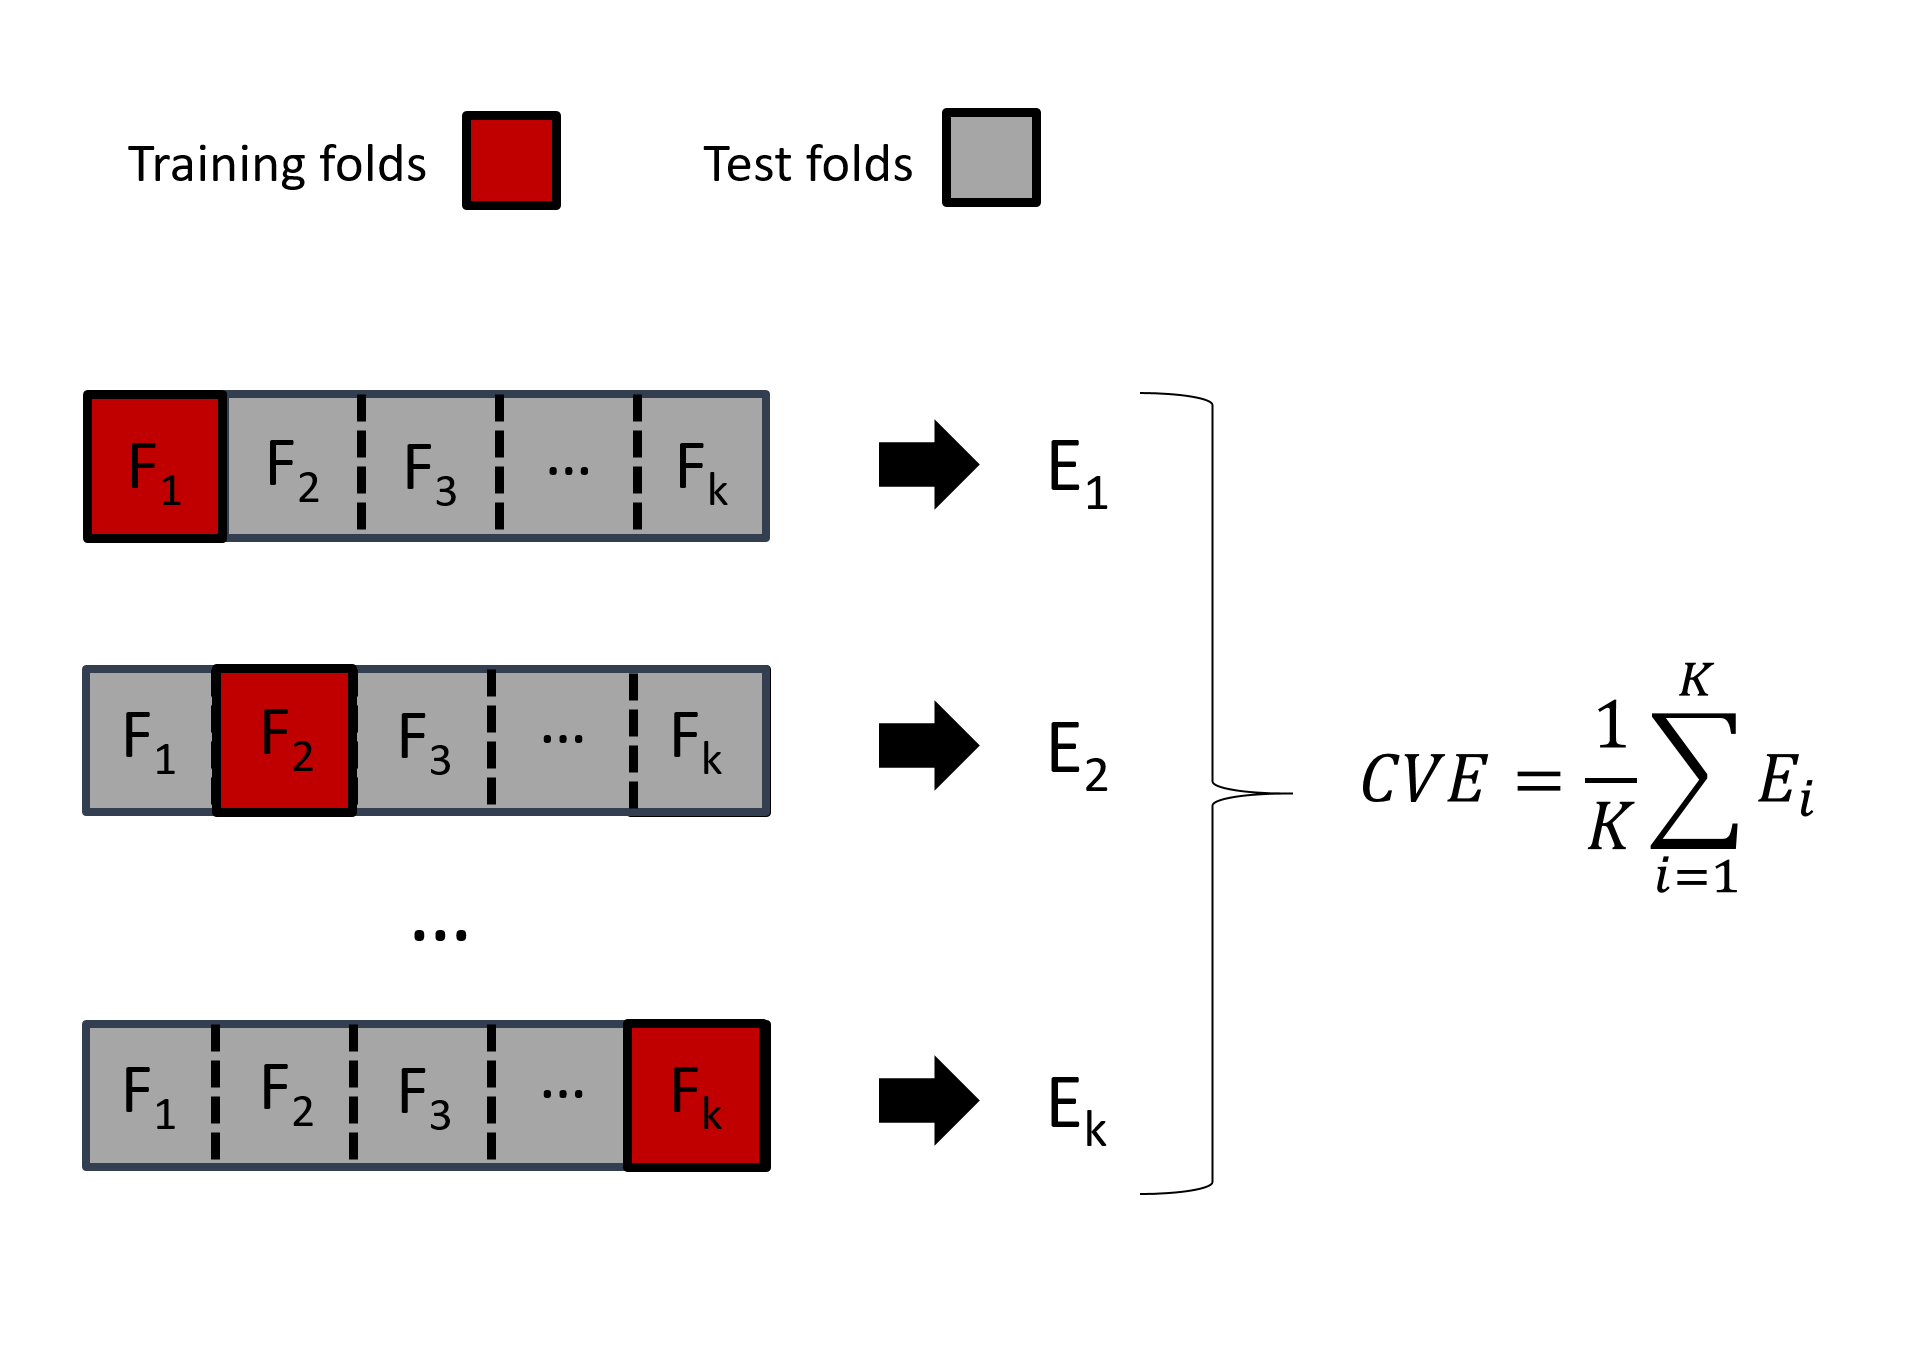
\includegraphics[width=0.7\textwidth]{figura39.png}
\caption[Scheme of a K-fold cross-validation procedure]{Scheme of a K-fold cross-validation procedure. At each iteration, one different fold acts as test fold while all the others act as training folds. At the end, the different prediction errors are averaged.}
\label{figura39}
\end{figure}


There are alternative ways to select or tune the hyperparameters apart from cross-validation \parencite{vujavcic2015computationally, zhang2010regularization}. These alternatives have the advantage of being computationally faster than cross-validation, but one important advantage of cross-validation is the possibility to estimate the standard error of the estimated cross-validated error performing the following steps: 

\vspace{15pt}
\begin{enumerate}
    \item \begin{equation}
    E_k=(y - \hat{y})^2
    \end{equation}
    \item \begin{equation}
    CVE=\frac{1}{K}\sum_{i=1}^{K}E_i
    \end{equation}
    \item \begin{equation}
    SD_{CVE}=\sqrt{var(E_1, E_2, \dots, E_k)}
    \end{equation}
    \item \begin{equation}
    SE_{CVE}=\frac{SD_{CVE}}{\sqrt{K}}
    \end{equation}
\label{secve}
\end{enumerate}

Performing a grid search on a three-dimensional hyperparameter step is computationally very demanding, so the fact that grid search is an embarrassingly parallel task \parencite{mcgibbon2016osprey} is exploited to parallelize the cross-validation procedure and be able to perform the repeated cross-validation in a reasonable time for medium and large data sets. Details on the parallelization algorithm will be presented in next chapter.


% ---------------------------------------------------------------------
% ---------------------------------------------------------------------
% ---------------------------------------------------------------------

\chapter[sNPLS package, a comprehensive software for N-PLS and sparse N-PLS analysis]{sNPLS package, a comprehensive software for \textit{N}-PLS and sparse \textit{N}-PLS analysis}
\label{chapter:package}


% ---------------------------------------------------------------------
% ---------------------------------------------------------------------
\section{Implementation of the sNPLS algorithm in \texttt{R}}
In this section the key functions of the code for the \textit{sNPLS} package implementing the sNPLS method will be exposed and commented. These include the main sNPLS function, the R-matrix function and the cross-validation functions. The full code for the package will be included in the appendix.

\subsection{Main algorithm}
This is the code of the main function of the package. It performs $N$-PLS regression as explained in \autoref{NPLSregression} and includes an L1-penalization step at the determination of $\textbf{\text{w}}^{J}$ and $\textbf{\text{w}}^{K}$ as explained in \autoref{NPLSpenalization}.
\vspace{15pt}
\begin{scriptsize}
\begin{lstlisting}[language=R, deletekeywords={scale, !=, <-, !, Q, qf, names, max, var}, otherkeywords={}, morekeywords={unfold3w}, caption=sNPLS main function]
sNPLS <- function(XN, Y, ncomp = 2, conver = 1e-16, max.iteration = 10000,
                  keepJ = rep(ncol(XN), ncomp), 
                  keepK = rep(rev(dim(XN))[1], ncomp),
                  scale.X=TRUE, center.X=TRUE, scale.Y=TRUE, center.Y=TRUE, 
                  silent = F) {
  
  mynorm <- function(x) sqrt(sum(diag(crossprod(x))))
  if (length(dim(Y)) == 3) Y <- unfold3w(Y)
  if (length(dim(XN)) != 3)
    stop("'XN' is not a three-way array")
  if (!is.null(rownames(XN)))
    y.names <- x.names <- rownames(XN) else {
    y.names <- x.names <- 1:dim(XN)[1]
    }
    if (!is.null(colnames(XN)))
      var.names <- colnames(XN) else {
      var.names <- paste("X.", 1:dim(XN)[2], sep = "")
      }
      if (!is.null(dimnames(XN)[[3]]))
        x3d.names <- dimnames(XN)[[3]] else {
        x3d.names <- paste("Z.", 1:dim(XN)[3], sep = "")
        }
        if (!is.null(colnames(Y)))
          yvar.names <- colnames(Y) else {
          yvar.names <- paste("Y.", 1:dim(Y)[2], sep = "")
          }
          if(!center.X) center.X <- rep(0, ncol(XN)*dim(XN)[3])
          if(!center.Y) center.Y <- rep(0, ncol(Y))
          if(!scale.X) scale.X <- rep(1, ncol(XN)*dim(XN)[3])
          if(!scale.Y) scale.Y <- rep(1, ncol(Y))
          
          # Matrices initialization
          Tm <- U <- Q <- WsupraJ <- WsupraK <- X <- P <- NULL
          Yorig <- Y
          Y <- scale(Y, center = center.Y, scale = scale.Y)
          y_center <- attr(Y, "scaled:center")
          y_scale <- attr(Y, "scaled:scale")
          B <- matrix(0, ncol = ncomp, nrow = ncomp)
          Gu <- vector("list", ncomp)
          S <- svd(Y)$d
          u <- Y[, S == max(S)]  #Column with the highest variance
          # Unfolding of XN en 2-D
          X <- unfold3w(XN)
          #Check for zero variance columns and fix them with some noise
          if(any(apply(X, 2, sd)==0)){
            X[,apply(X, 2, sd)==0] <- apply(X[,apply(X, 2, sd)==0, drop=F], 
                                            2, function(x) jitter(x))
          }
          # Center and scale
          Xd <- scale(X, center = center.X, scale = scale.X)
          x_center <- attr(Xd, "scaled:center")
          x_scale <- attr(Xd, "scaled:scale")
          
          # Main loop for each component
          for (f in 1:ncomp) {
            nj <- ncol(XN) - keepJ[f]
            nk <- dim(XN)[3] - keepK[f]
            it = 1
            while (it < max.iteration) {
              Zrow <- crossprod(u, Xd)
              Z <- matrix(Zrow, nrow = dim(XN)[2], ncol = dim(XN)[3])
              svd.z <- svd(Z)
              wsupraj <- svd.z$u[, 1]
              # L1 penalization for wsupraj
              if (nj != 0) {
                wsupraj <- ifelse(abs(wsupraj) > 
                                  abs(wsupraj[order(abs(wsupraj))][nj]),
                                  (abs(wsupraj) - 
                                  abs(wsupraj[order(abs(wsupraj))][nj])) *
                                  sign(wsupraj), 0)
              }
              ##########
              wsuprak <- svd.z$v[, 1]
              # L1 penalization for wsuprak
              if (nk != 0) {
                wsuprak <- ifelse(abs(wsuprak) > 
                                  abs(wsuprak[order(abs(wsuprak))][nk]),
                                  (abs(wsuprak) - 
                                  abs(wsuprak[order(abs(wsuprak))][nk])) *
                                  sign(wsuprak), 0)
              }
              ##########
              tf <- Xd %*% kronecker(wsuprak, wsupraj)
              qf <- crossprod(Y, tf)/mynorm(crossprod(Y, tf))
              uf <- Y %*% qf
              if (sum((uf - u)^2) < conver) {
                if (!silent) {
                  cat(paste("Component number ", f, "\n"))
                  cat(paste("Number of iterations: ", it, "\n"))
                }
                it <- max.iteration
                Tm <- cbind(Tm, tf)
                WsupraJ <- cbind(WsupraJ, wsupraj)
                WsupraK <- cbind(WsupraK, wsuprak)
                bf <- MASS::ginv(crossprod(Tm)) %*% t(Tm) %*% uf
                B[1:length(bf), f] <- bf
                Q <- cbind(Q, qf)
                U <- cbind(U, uf)
                TM <- MASS::ginv(crossprod(Tm)) %*% t(Tm)
                WkM <- MASS::ginv(crossprod(WsupraK)) %*% t(WsupraK)
                WjM <- MASS::ginv(crossprod(WsupraJ)) %*% t(WsupraJ)
                Gu[[f]] <- TM %*% X %*% kronecker(t(WkM), t(WjM))
                P[[f]] = t(as.matrix(Gu[[f]]) %*% 
                         t(kronecker(WsupraK, WsupraJ)))
                Y <- Y - Tm %*% bf %*% t(qf)
                S <- svd(Y)$d
                u <- Y[, S == max(S)]
              } else {
                u <- uf
                it <- it + 1
              }
            }
          }
          Yadjsc <- Tm %*% B %*% t(Q)
          Yadj <- Yadjsc * y_scale + y_center
          SqrdE <- sum((Yorig - Yadj)^2)
          rownames(WsupraJ) <- var.names
          rownames(WsupraK) <- x3d.names
          rownames(Q) <- yvar.names
          rownames(Tm) <- rownames(U) <- x.names
          colnames(Tm) <- colnames(WsupraJ) <- colnames(WsupraK) <- 
                          colnames(B) <- colnames(U) <- colnames(Q) <- 
                          names(Gu) <- names(P) <- paste("Comp.", 1:ncomp)
          output <- list(T = Tm, Wj = WsupraJ, Wk = WsupraK, B = B, U = U, 
                         Q = Q, P = P, Gu = Gu, ncomp = ncomp, Yadj = Yadj, 
                         SqrdE = SqrdE, 
                         Standarization = list(ScaleX = x_scale, 
                                               CenterX = x_center,
                                               ScaleY = y_scale, 
                                               CenterY = y_center))
          class(output)<-"sNPLS"
          return(output)
}
\end{lstlisting}
\end{scriptsize}

Lines 1-5 define the parameters of the function. Parameters with default values have that value assigned after an equal sign. Line 7 defines an internal function for normalization. Lines 8-30 check for inconsistencies in the data structure, unfold \textbf{\underline{Y}} (when necessary) and assign variable names. After this, all necessary matrices are initiallized in lines 33-52, \textbf{\underline{X}} is unfolded into \textbf{X} and optional centering and scaling is applied on \textbf{Y} and \textbf{X}. The following lines (55-113) correspond to the $N$-PLS algorithm described in \autoref{NPLSpenalization}. Last lines (114-133) include the estimation of \textbf{Y}, the computing of the squared prediction error, and the generation of the output object of the function, defined as an S3 object of class \textit{sNPLS}. This object includes the different output matrices of the model as well as all the information regarding the model fit such as centering on \textbf{X} and/or \textbf{Y} and used values for the hyperparameters. 


\subsection{R matrix computation}
\label{rmatrixf}
This function is used for computing the coefficients used for prediction of \textbf{Y} in the \texttt{predic.sNPLS} function.
\vspace{15pt}
\begin{scriptsize}
\begin{lstlisting}[language=R, deletekeywords={scale, !=, <-, !, Q, qf, names, max, var}, otherkeywords={}, morekeywords={unfold3w}, caption=R matrix function]
Rmatrix<-function(x) {
  WsupraK <- x$Wk
  WsupraJ <- x$Wj
  R <- matrix(nrow = dim(x$Wj)[1] * dim(x$Wk)[1], ncol = x$ncomp)
  ncomp <- x$ncomp
  kroneckers<-sapply(1:x$ncomp, function(x) {
                     kronecker(WsupraK[, x], WsupraJ[, x]))
                     }
  tkroneckers<-apply(kroneckers, 2, function(x) t(x))
  R[,1] <- kroneckers[,1]
  if(ncomp>1){
    for(i in 2:ncomp){
      pi <- pi0 <- Matrix::Matrix(diag(dim(R)[1]), sparse=TRUE)
      for (j in 1:(i - 1)) {
        pi <- Matrix::Matrix(pi %*% pi0 - kroneckers[,j] %*% 
        t(tkroneckers[,j]), sparse=TRUE)
      }
      w <- kroneckers[, i]
      pi <- pi %*% w
      R[, i] <- Matrix::as.matrix(pi)
    }
  }
  return(R)
}
\end{lstlisting}
\end{scriptsize}

Of note, most of the computations performed inside the \texttt{Rmatrix} function make use of sparse matrices (lines 12-19), taking advantage of the sparsity created by the \texttt{sNPLS} function when adjusting the model to greatly reduce computing times. The \texttt{Rmatrix} function is an internal function (not exported to the end user) called by the \texttt{sNPLS} and \texttt{predict.sNPLS} functions to get the regression coefficients in order to be able to perform predictions from new \textbf{\underline{X}} as explained in \textcite{leardi2005multi}:

The \textbf{R} matrix is defined as:

\begin{equation}
    \textbf{\text{R}}=[\textbf{\text{w}}_1(\textbf{\text{I}}-\textbf{\text{w}}_1\textbf{\text{w}}^T_1)\textbf{\text{w}}_2 \dots (\prod_{f=1}^{F-1}(\textbf{\text{I}}-\textbf{\text{w}}_f\textbf{\text{w}}^T_f)\textbf{\text{w}}_F)]
\end{equation}

From this, it derives that

\begin{equation}
    \textbf{\text{T}}=\textbf{\text{XR}}
\end{equation}

So, from the equation

\begin{equation}
    \hat{\textbf{\text{y}}}=\textbf{\text{Tb}}
\end{equation}

it is obtained

\begin{equation}
    \textbf{\text{b}}_{NPLS}=\textbf{\text{Rb}}
\end{equation}

\subsection{Cross validation (\texttt{cv\_snpls})}
The \texttt{cv\_snpls} function is used to estimate the best combination of parameters for adjusting sNPLS models using $K$-fold cross-validation. Since the hyperparameter space can be huge when considering a grid search for three different hyperparameters, it has been parallelized using the \textit{parallel} package to greatly speed up computation times. For simple problems or small data sets it can also be run in single thread mode.
\vspace{15pt}
\begin{scriptsize}
\begin{lstlisting}[language=R, deletekeywords={scale, !=, <-, !, Q, qf, names, max, var, drop, se, search.grid, mean, grid, search}, otherkeywords={}, morekeywords={unfold3w}, caption=Cross validation function]
cv_snpls <- function(X_npls, Y_npls, ncomp = 1:3, keepJ = 1:ncol(X_npls),
                     keepK = 1:dim(X_npls)[3], nfold = 10, parallel = TRUE, 
                     free_cores = 2, ...) {
    #Creation of cluster and exportation of data to the nodes
    if (parallel & (parallel::detectCores()>1)) {
        cl <- parallel::makeCluster(max(2, 
                                    parallel::detectCores() - free_cores))
        parallel::clusterExport(cl, list(deparse(substitute(X_npls)),
                                         deparse(substitute(Y_npls))))
        parallel::clusterCall(cl, function() require(sNPLS))
    }
  if(length(dim(Y_npls)) == 3) Y_npls <- unfold3w(Y_npls)
  top <- ceiling(dim(X_npls)[1]/nfold)
    foldid <- sample(rep(1:nfold, top), dim(X_npls)[1], replace = F)
    #Expansion of hyperparameters grid
    search.grid <- expand.grid(list(ncomp = ncomp, 
                                    keepJ = keepJ, 
                                    keepK = keepK))
    SqrdE <- numeric()
    #Main function
    applied_fun <- function(y) {
        sapply(1:nfold, function(x) {
            tryCatch(cv_fit(xtrain = X_npls[x != foldid, , ],
                            ytrain = Y_npls[x != foldid, , drop = FALSE],
                            xval = X_npls[x == foldid, , ],
                            yval = Y_npls[x == foldid, , drop = FALSE],
                            ncomp = y["ncomp"],
                            keepJ = rep(y["keepJ"], y["ncomp"]),
                            keepK = rep(y["keepK"], y["ncomp"]), ...),
                     error=function(x) NA)
          })
    }
    #Parallelization of main function
    if (parallel) {
        cv_res <- parallel::parApply(cl, search.grid, 1, applied_fun)
        parallel::stopCluster(cl)
    } else cv_res <- pbapply::pbapply(search.grid, 1, applied_fun)
    cv_mean <- apply(cv_res, 2, function(x) mean(x, na.rm = TRUE))
    cv_se <- apply(cv_res, 2, function(x) sd(x, na.rm=TRUE)/sqrt(nfold))
    best_model <- search.grid[which.min(cv_mean), ]
    output <- list(best_parameters = best_model, cv_mean = cv_mean,
                   cv_se = cv_se, cv_grid = search.grid)
    class(output)<-"cvsNPLS"
    return(output)
}
\end{lstlisting}
\end{scriptsize}

Of note, regarding the \texttt{cv\_snpls} function, is the code related to the parallelization of the procedure using the \texttt{parallel} package (lines 5-11 for the definition of the cluster and lines 34-37 for the execution of the parallelized procedure). The function makes use of the \texttt{parApply} function, which splits the search grid in $n$ nodes and runs the cross-validation procedure on each split independently, combining all results at the end of the computations. Lines 21-32 of the function correspond to the cross-validation procedure defined in \autoref{hyperparameters}.

\subsection{Repeated Cross validation (\texttt{repeat\_cv})}
\label{repeatcv}
The \texttt{repeat\_cv} calls the \texttt{cv\_snpls} function repeated times, but it changes the way of parallelizing the computations. 

In this function, each \texttt{cv\_snpls} call is run in single thread mode, but assigned to a different node. So, instead of on subsets of the search grid, the parallelization is performed on repetitions of the procedure on the whole grid. This handling of the parallelization allows for a more efficient distribution of the jobs across the different nodes of the defined cluster, assuming the number of repetitions is greater than the number of folds $K$ of the $K$-fold cross-validation procedure.

\vspace{12pt}
\begin{lstlisting}[language=R, deletekeywords={scale, !=, <-, !, Q, qf, names, max, var, drop, se, search.grid, mean, grid, search, rep, repeat}, otherkeywords={}, morekeywords={unfold3w, pbreplicate, parSapply}, caption=Repeated cross validation function]
repeat_cv<-function(X_npls, Y_npls, ncomp = 1:3, keepJ = 1:ncol(X_npls), 
                    keepK = 1:dim(X_npls)[3], nfold = 10, 
                    parallel = TRUE, free_cores = 2, times=30, ...){
  #Definition of the cluster and exportation of data to the nodes
  if(parallel & (parallel::detectCores()>1)){
    cl <- parallel::makeCluster(max(2, 
                                parallel::detectCores() - free_cores))
    parallel::clusterExport(cl, list(deparse(substitute(X_npls)), 
                                     deparse(substitute(Y_npls))))
    parallel::clusterCall(cl, function() require(sNPLS))
    #Parallelization of the repetitions of K-fold cross-validation
    rep_cv<-parallel::parSapply(cl, 1:times, function(x){
                                cv_snpls(X_npls, Y_npls, ncomp=ncomp, 
                                keepJ = keepJ, keepK = keepK, 
                                parallel = FALSE, nfold = nfold, ...))
                                }
    parallel::stopCluster(cl)
  } else {
    #Single threaded version (Not use, slow)
    rep_cv<-pbapply::pbreplicate(times, cv_snpls(X_npls, Y_npls, 
                                 ncomp=ncomp, keepJ = keepJ, 
                                 keepK = keepK, parallel = FALSE, 
                                 nfold = nfold, ...))
  }
  resdata<-data.frame(ncomp=sapply(rep_cv[1,], function(x) x[[1]]), 
                      keepJ=sapply(rep_cv[1,], function(x) x[[2]]),
                      keepK=sapply(rep_cv[1,], function(x) x[[3]]))
  class(resdata)<-c("repeatcv", "data.frame")
  return(resdata)
}
\end{lstlisting}

\section{The sNPLS package}
In the following section, the use of the different functions of the \texttt{sNPLS} package will be presented, as well as examples of their application to the different parts of the analysis in two data sets. A special emphasis will be given to the main \texttt{sNPLS} function, as well as to both cross-validation functions for the selection of the hyperparameters and to the different plot functions for the interpretation of results. This section is based on the published paper for the \textit{sNPLS} package \parencite{hervas2018sparse}.

\subsection{Functions}
\subsubsection{\texttt{sNPLS} function}
Function \texttt{sNPLS} is used to fit $N$-PLS and sNPLS models to three-way data, depending on the input settings of the algorithm. The following \textit{R} code shows an example of a model fit to a simulated three-way dataset with fifty observations ($I$), 50 variables ($J$) and three elements in the third mode ($K$).
\vspace{15pt}
\begin{lstlisting}[basicstyle=\small, language=Python, morekeywords={array, matrix, sNPLS, rep, rpois, rnorm}]
R> library("sNPLS")
R> X_npls <- array(rpois(7500, 10), dim=c(50, 50, 3))
R> Y_npls <- matrix(2+0.4*X_npls[,5,1]+0.7*X_npls[,10,1]- 
+    0.9*X_npls[,15,1] + 0.6*X_npls[,20,1] - 0.5*X_npls[,25,1]+
+    rnorm(50), ncol=1)
R> fit <- sNPLS(X_npls, Y_npls, ncomp=3, keepJ = rep(2,3), 
+    keepK = rep(1,3))
\end{lstlisting}

Note that the function \texttt{sNPLS} needs a $N$-way array for \textbf{\underline{X}} and an $N$-way array, a two-dimensional matrix or a numeric vector for \textbf{Y} as inputs. If data is in another format the function will stop and throw an error. In the following paragraph, a generic call with a short description of each of the arguments of the function is presented.
\vspace{15pt}
\begin{lstlisting}[basicstyle=\small, language=R, deletekeywords={max, scale}, morekeywords={array, matrix, rep, rpois, rnorm, function}, otherkeywords={}]
sNPLS(XN, Y, ncomp = 2, conver = 1e-16, 
+    max.iteration = 10000, keepJ = rep(ncol(XN), ncomp), 
+    keepK = rep(rev(dim(XN))[1], ncomp), scale.X=TRUE, 
+    center.X=TRUE, scale.Y=TRUE, center.Y=TRUE, silent = F)
\end{lstlisting}
\vspace{10pt}
\begin{itemize}[leftmargin=2.5cm]
\item[XN] $N$-dimensional array containing the predictors
\item[Y] Array containing the response(s)
\item[ncomp] Number of components to use in the projection
\item[conver] Convergence criterion
\item[max.iteration] Maximum allowed number of iterations to achieve convergence
\item[keepJ] Number of variables to keep at each component. If all variables are kept, NPLS regression is performed, if any variable is removed then sNPLS is performed.
\item[keepK] Number of elements of the third mode to keep at each component.
\item[scale.X] Perform scaling on \textbf{\text{X}}?
\item[center.X] Perform centering on \textbf{\text{X}}?
\item[scale.Y] Perform scaling on \textbf{\text{Y}}?
\item[center.Y] Perform centering on \textbf{\text{Y}}?
\item[silent] Allows to choose if information regarding number of iterations should be displayed
\end{itemize}
\vspace{7pt}
The function \texttt{sNPLS} produces an \texttt{S3 sNPLS} object with defined \texttt{coef}, \texttt{predict} and \texttt{plot} methods that will be discussed later. The object consists of a list containing the following components: [1-6] The \textbf{T}, $\textbf{\text{W}}^{J}$, $\textbf{\text{W}}^{K}$, \textbf{B} (regression coefficients between \textbf{\underline{X}} and \textbf{\underline{Y}}), \textbf{Y} and \textbf{Q} matrices, [7-8] \textbf{P} and \textbf{G}u (the unfolded \textbf{G} core array of the Tucker decomposition), [9] The number of components, [10] Fitted values, [11] Squared error, [12] Scale and centering information performed on \textbf{\underline{X}} and \textbf{Y}.

\subsubsection{\texttt{cv\_sNPLS} and \texttt{repeat\_cv} functions}
Selecting parameter values for the \texttt{sNPLS} function requires choosing values for the number of components, the number of variables to select and the number of elements of the third mode to select. An appropriate way of selecting these parameters is performing a grid search with cross-validation. The function \texttt{cv\_snpls} performs cross-validation on a grid of different \texttt{ncomp}, \texttt{keepJ} and \texttt{keepK} values estimating $RMSE$ (Root Mean Square Error) for each combination of values and selecting the best set producing the lowest $RMSE$.

\vspace{15pt}
\begin{lstlisting}[basicstyle=\small, language=Python, deletekeywords={max, scale}, morekeywords={array, matrix, rep, rpois, rnorm, function, cv_snpls}, otherkeywords={}]
R> X_npls<-array(rpois(7500, 10), dim=c(50, 50, 3))
R> Y_npls<-matrix(2+0.4*X_npls[,5,1]+0.7*X_npls[,10,1]-
+    0.9*X_npls[,15,1]+0.6*X_npls[,20,1]- 0.5*X_npls[,25,1]+
+    rnorm(50), ncol=1)
R> cv1<- cv_snpls(X_npls, Y_npls, ncomp=1:2, keepJ = 1:10, 
+    keepK = 1:3, parallel = FALSE)
\end{lstlisting}

The generic call for \texttt{cv\_snpls} is the following:
\vspace{15pt}
\begin{lstlisting}[basicstyle=\small, language=R, deletekeywords={max, scale}, morekeywords={array, matrix, rep, rpois, rnorm, function, cv_snpls}, otherkeywords={}]
cv_snpls(X_npls, Y_npls, ncomp = 1:3, keepJ = 1:ncol(X_npls),
+   keepK = 1:dim(X_npls)[3], nfold = 10, parallel = FALSE)
\end{lstlisting}

It contains the same parameters as \texttt{sNPLS} but now admits vectors of values for each parameter in \texttt{ncomp}, \texttt{keepJ} and \texttt{keepK}. Since grid search can be computationally intensive, it makes use of the \texttt{parallel} package. Being able to perform computations in parallel greatly reduces running times, being able to finish between 1.5 and 6 times faster in an eight-core computer, depending on the data set. Parallel mode is activated by setting \texttt{parallel} argument to \texttt{TRUE} and selecting a suitable number of free cores. As explained in \autoref{repeatcv}, in the case of \texttt{cv\_snpls}, the parallelization applies to the grid search, not to the different folds of the cross-validation.

To further reduce computation times and improve memory use, sparse matrices from the \texttt{R} package \texttt{Matrix} \parencite{matrixsparse} are used whenever possible in the matrix multiplication steps of the function. Sparse matrices achieve these goals by using an alternative representation to that of dense matrices: instead of being stored as two-dimensional arrays, only their non-zero values are stored, along with an index linking these values with their location in the matrix. The function \texttt{cv\_snpls} returns a \texttt{cvsnpls} object which is a list with a component containing the best combination parameters and other components containing information about the grid and its corresponding \texttt{RMSE}. \texttt{cv\_snpls} objects  can be plotted for better interpretation of the results. The resulting plot is a grid of scatterplots with the different combinations of \texttt{keepJ}, \texttt{keepK} and \texttt{ncomp} and their resulting cross-validation errors (\autoref{figura04}).

\vspace{10pt}
\begin{figure}[!ht]
	\centering
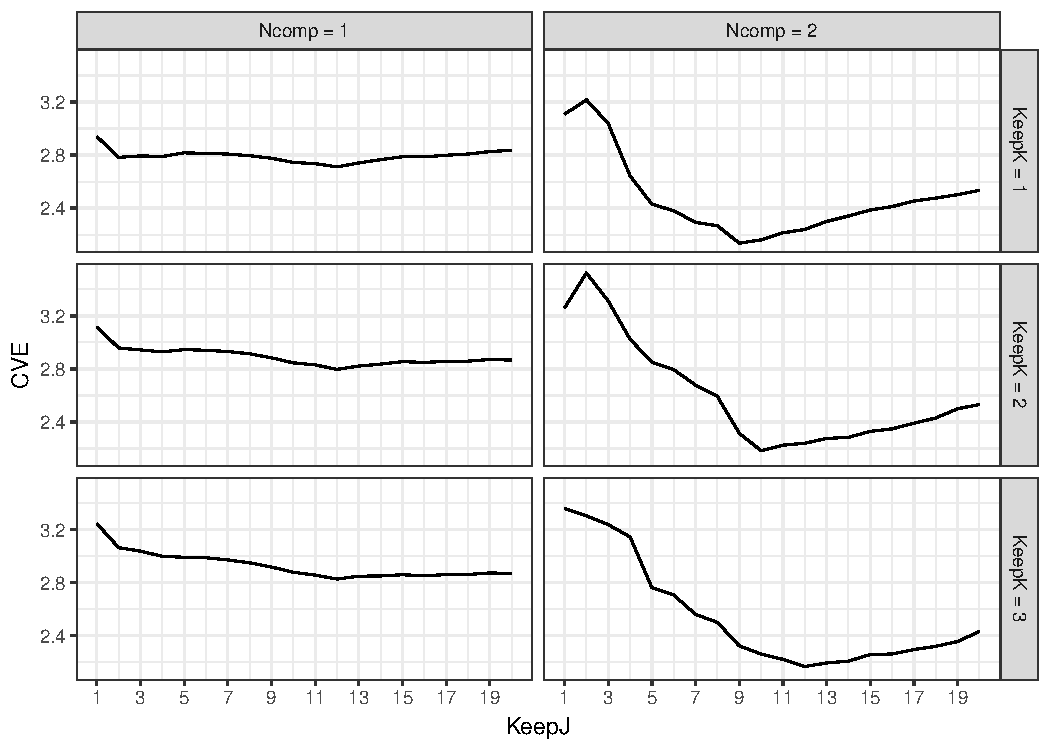
\includegraphics[width=0.85\textwidth]{figura04.pdf}
\caption[Results of cross-validation]{Results of cross-validation. Lines depicting the cross-validated error (CVE) for each combination of the parameters are presented in a grid layout combining \texttt{KeepJ} values (number of variables selected), \texttt{KeepK} values (number of elements of the third mode) and \texttt{Ncomp} values (number of components).}
\label{figura04}
\end{figure}
\vspace{10pt}

A known issue of cross-validation is the variance in its results \parencite{krstajic2014cross}, which entails that different runs of the cross-validation procedure can yield different results regarding the estimated best set of parameters and, more importantly, that the cross-validation procedure can overfit in the estimation of the error. This overfitting would entail that repeating the same cross-validation procedure on another sample of the population would yield totally different results. A reasonable solution is performing repeated cross-validation and selecting the most frequently selected set of parameters along a round of different runs. The function \texttt{repeat\_cv} performs repeated cross-validation by calling the function \texttt{cv\_snpls} repeated times and storing each result in a \texttt{data.frame} object. The syntax is the same as in \texttt{cv\_snpls} with an extra argument \texttt{times} for specifying the number of repetitions to perform. In the case of \texttt{repeat\_cv} the parallelization applies to the replicates instead of applying to the grid search. The following code explains how to perform repeated cross-validation with \texttt{repeat\_cv}.

\vspace{15pt}
\begin{lstlisting}[basicstyle=\small, language=Python, deletekeywords={max, scale}, morekeywords={array, matrix, rep, rpois, rnorm, function, repeat_cv}, otherkeywords={}]
R> repcv <- repeat_cv(X_npls, Y_npls, ncomp=1:2, keepJ = 1:10, 
+    keepK = 1:3, parallel = FALSE, times=10)
\end{lstlisting}

The result of the \texttt{repeat\_cv} call is a \texttt{data.frame} storing the results (best combination of \texttt{ncomp}, \texttt{keepJ} and \texttt{keepK} of each cross-validation repetition (\autoref{output1}). 

\vspace{15pt}
\begin{lstlisting}[basicstyle=\small, language=Python]
R> repcv
\end{lstlisting}

\vspace{5pt}
\begin{lstlisting}[basicstyle=\small, backgroundcolor=\color{output}, numbers=none, label={output1}, language=Python, caption=Results of \texttt{repeat\_cv} function.]
   ncomp keepJ keepK
1      2     9     1
2      2     9     1
3      2    10     1
4      2     9     1
5      2    11     2
6      2    12     1
7      2     7     1
8      2    10     1
9      2     8     1
10     2    12     2
\end{lstlisting}

This output can be presented as a cross-tabulation table with the absolute frequencies of each combination of the different parameters (\autoref{output2}. In this example, the table shows that the combination \texttt{ncomp}=2, \texttt{keepJ}=9 and \texttt{keepK}=1 is the most recurrent (3 out of 10 repetitions), followed by the combination \texttt{ncomp}=2, \texttt{keepJ}=10 and \texttt{keepK}=1 with two repetitions and five other different combinations with just one occurrence each. It can also be noticed that none of the best combinations included only one component.

\vspace{15pt}
\begin{lstlisting}[basicstyle=\small, language=Python, deletekeywords={max, scale}, morekeywords={ftable, table}, otherkeywords={}]
R> ftable(table(repcv))
\end{lstlisting}

\begin{lstlisting}[basicstyle=\small, backgroundcolor=\color{output}, numbers=none, label={output2}, language=Python, caption=Cross-tabulation table of the results of \texttt{repeat\_cv}.]
            keepK 1 2
ncomp keepJ          
2     7           1 0
      8           1 0
      9           3 0
      10          2 0
      11          0 1
      12          1 1
\end{lstlisting}

Results of the \texttt{repeat\_cv} function can also be plotted to obtain a kernel density plot, which can be one-, two- or three-dimensional depending of the number of constant parameters obtained in the repeated cross-validation procedure. This density plot depicts the most frequently selected parameters (\autoref{figura05}). 
\vspace{10pt}
\begin{figure}[hbtp]
	\centering
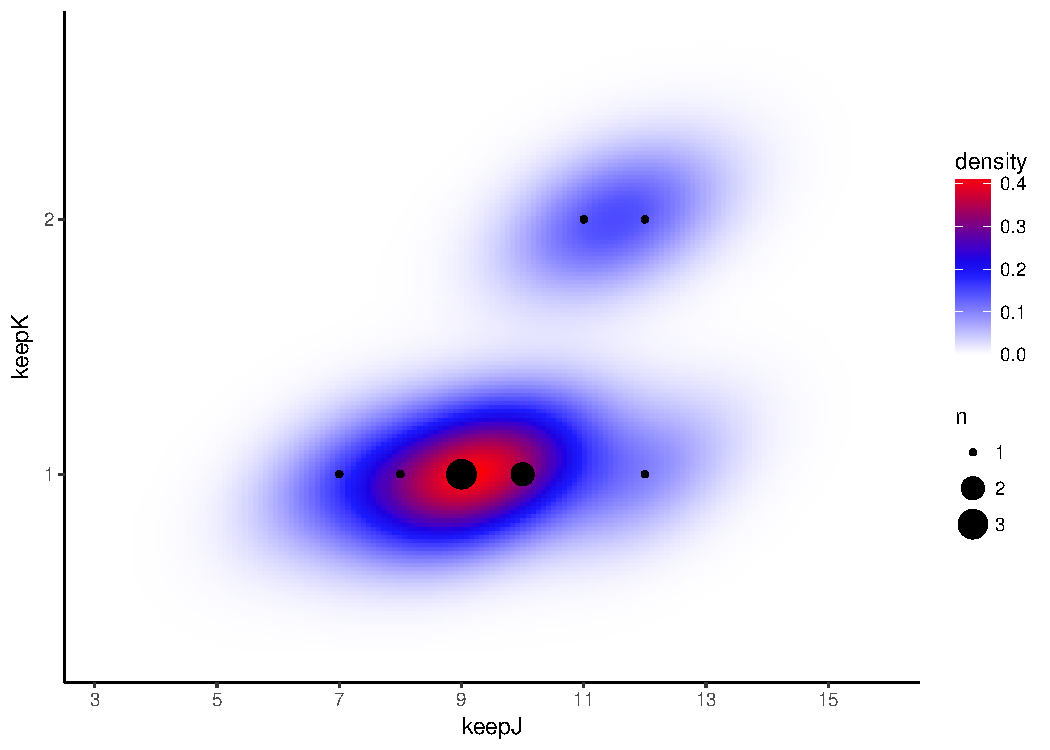
\includegraphics[width=0.7\textwidth]{figura05.pdf}
\caption[Kernel density plot with the results of repeated cross-validation]{Kernel density plot with the result of the repeated cross-validation. Highest density lies around \texttt{keepJ}=9 and \texttt{keepK}=1. Points scaled in size by frequency of appearance are additionally included on top of the density plot. The number of components is not represented since it was constant at 2 in all repetitions of the cross-validation.}
\label{figura05}
\end{figure}

In this example, according to the plot, the most likely combination after all repetitions of the cross-validation was between 9 and 10 in the case of \texttt{keepJ} and \texttt{keepK}=1. Since the optimal number of components did not vary along all the repetitions, this parameter is not represented in the plot. Instead, the message \texttt{'ncomp is(are) constant with a value of 2'} is returned by the function. The density plot leads to a similar interpretation of the results as the cross-tabulation table, but the smoothing can result in more sensible estimates in the case of multiple and/or wide spread modes. It also provides a visual measure of the uncertainty in the selection of the best combination of parameters.

\subsubsection{Full example functionality}
To exhibit all package functionality, next it is provided a complete analysis of the \texttt{bread} dataset \parencite{bro1998multi} included in the \textit{sNPLS} package. This data set consists on data of five different breads that were baked in duplicate giving a total of ten samples. Eight different judges assessed the breads with respect to eleven different sensorial attributes. The data can be regarded as a three-way array (10 x 11 x 8). The data are quite noisy as opposed to, e.g., spectral data. The salt content of each bread was also measured and it is considered as the response variable \textbf{y}.
\vspace{15pt}
\begin{lstlisting}[basicstyle=\small, language=Python, morekeywords={data, repeat_cv}]
R> data(bread)
R> Xbread <- bread$Xbread
R> Ybread <- bread$Ybread
R> cv_bread <- repeat_cv(Xbread, Ybread, ncomp=1:3, keepJ = 1:11,   
+    keepK = 1:8, parallel = FALSE, times=50, nfold=3)
\end{lstlisting}

After importation of the data set and preparation of the \textbf{\underline{X}} array and \textbf{y} vector (first three lines of the code above), repeated cross-validation is performed on the data to select the optimal combination of hyperparameters. 50 repetitions of 3-fold cross-validation should be enough to get stable estimates, but using such a large number of repetitions would increase computing times dramatically. Therefore, using the option \texttt{parallel=TRUE} when performing repeated cross-validation is recommended. Results of this procedure yield a cross-tabulation table with the appearance frequencies for each combination of parameters \autoref{output3}.

\vspace{15pt}
\begin{lstlisting}[basicstyle=\small, language=Python, morekeywords={ftable, table}]
R> ftable(table(cv_bread)) 
\end{lstlisting}

\begin{lstlisting}[basicstyle=\small, backgroundcolor=\color{output}, numbers=none, label={output3}, language=Python, caption=\texttt{repeat\_cv} results for the \texttt{bread} data set.]
            keepK 1 2 3 4 5 6 7 8
ncomp keepJ                      
1     1           1 2 2 4 3 3 1 1
      2           0 0 1 1 2 1 0 2
2     1           0 0 0 0 0 0 0 1
      2           0 0 0 0 0 0 0 2
      3           0 0 0 0 0 1 0 4
      4           0 0 0 0 0 0 1 1
      5           1 0 0 0 0 0 0 1
      6           0 0 0 0 0 0 1 0
      7           0 0 0 0 0 0 1 0
      8           0 0 0 0 0 0 0 2
      9           0 0 0 0 0 0 0 1
3     1           0 0 1 0 0 2 0 1
      2           0 0 0 0 0 0 1 1
      3           0 0 0 0 0 0 0 1
      5           0 0 0 0 0 0 0 1
\end{lstlisting}    
      
This table shows that there are two possible combinations of parameters that are almost equally selected by cross-validation. One is \texttt{ncomp}=1, \texttt{keepJ}=1 and \texttt{keepK}=4 and the other is \texttt{ncomp}=2, \texttt{keepJ}=3 and \texttt{keepK}=8, both with 4 appearances out of 50 repetitions. Also most of the other combinations are close to one of these two mentioned 'hotspots'. A plot of the \texttt{cv\_bread} object (\autoref{figura06}) reveals a similar information with a representation of a sliced three-dimensional kernel density estimate.


\begin{figure}[!ht]
	\centering
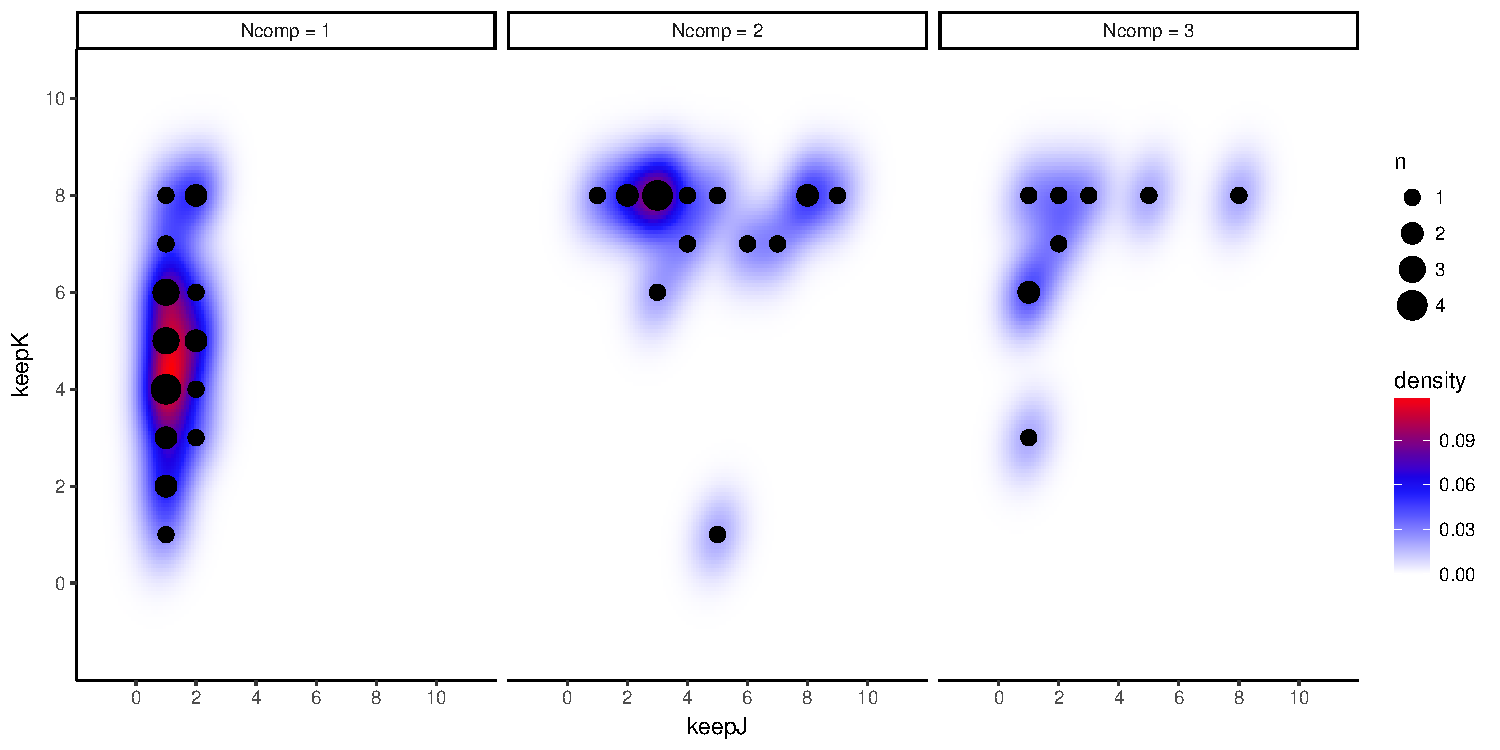
\includegraphics[width=0.98\textwidth]{figura06.pdf}
\caption[Results of the repeated cross-validation function performed on the \texttt{bread} dataset]{Results of the repeated cross-validation function performed on the \texttt{bread} dataset. The plot consists on the faceted representation of a three-dimensional density plot sliced in different planes (one per number of components). The kernel density estimation is created with the observed frequencies of the combinations of the different parameters. Additionally, points scaled in size by frequency of appearance are added to the density plots.}
\label{figura06}
\end{figure}

Next step would be fitting the \texttt{sNPLS} model using the \texttt{sNPLS} function with the selected set of parameters. As discussed before, the results point to two possible combinations and, based on the density plot, the option with \texttt{ncomp}=1, \texttt{keepJ}=1 and \texttt{keepK}=4 seems more likely. Nevertheless, the combination with \texttt{ncomp}=2 will be used to get working examples of the \texttt{plot} function (which needs, at least, two dimensions). It is important to take into account that \texttt{keepJ} and \texttt{keepK} have to be specified for each component, so they must be a vector of length equal to the number of components. Note that, in this case, the same number of attributes and judges for each component have been chosen, although this is not necessarily the case.

\vspace{15pt}
\begin{lstlisting}[basicstyle=\small, language=Python, morekeywords={sNPLS, rep}]
R> fit <- sNPLS(Xbread, Ybread, ncomp = 2, keepJ = rep(3, 2), 
+    keepK = rep(8, 2), silent = F)
\end{lstlisting}   

The summary of the fit shows the number of components, the estimated squared error and a matrix with rows corresponding to attributes (second mode) and columns corresponding to judges (third mode). In this matrix there are five rows with non-zero coefficients which correspond to the 4th, 6th 7th 8th and 9th attributes from all the judges (no selection is performed on the third mode).

\vspace{15pt}
\begin{lstlisting}[basicstyle=\small, language=Python, morekeywords={summary}]
R> summary(fit)
\end{lstlisting}   

\begin{lstlisting}[basicstyle=\small, backgroundcolor=\color{output}, numbers=none, label={output4}, language=R, deletekeywords={model}, caption=Summary with the coefficients of the fitted model.]

sNPLS model with 2 components and squared error of 0.047 
 
Coefficients: 
        Z.1    Z.2    Z.3    Z.4    Z.5    Z.6    Z.7    Z.8
X.1   0.000  0.000  0.000  0.000  0.000  0.000  0.000  0.000
X.2   0.000  0.000  0.000  0.000  0.000  0.000  0.000  0.000
X.3   0.000  0.000  0.000  0.000  0.000  0.000  0.000  0.000
X.4  -0.041 -0.041 -0.043 -0.049 -0.074 -0.040 -0.042 -0.029
X.5   0.000  0.000  0.000  0.000  0.000  0.000  0.000  0.000
X.6   0.019  0.026  0.024  0.027  0.021  0.025  0.018  0.036
X.7   0.070  0.089  0.086  0.095  0.087  0.088  0.069  0.115
X.8  -0.030 -0.038 -0.037 -0.041 -0.038 -0.038 -0.030 -0.050
X.9  -0.009 -0.009 -0.010 -0.011 -0.017 -0.009 -0.009 -0.006
X.10  0.000  0.000  0.000  0.000  0.000  0.000  0.000  0.000
X.11  0.000  0.000  0.000  0.000  0.000  0.000  0.000  0.000
\end{lstlisting}  

To better understand and interpret the results, the plot function can be used to display different visualizations of the results. Values of the \textbf{T} (\autoref{figura07}), \textbf{U} (\autoref{figura08}), $\textbf{\text{W}}^{J}$ (\autoref{figura09} and \autoref{figura11}), and $\textbf{\text{W}}^{K}$ (\autoref{figura10} and \autoref{figura12}) matrices can be plotted by changing the \texttt{type} parameter of the function. 1st and 2nd components are plotted by default, but they can be changed using the \texttt{comps} parameter.

\vspace{15pt}
\begin{lstlisting}[basicstyle=\small, language=Python]
R> plot(fit, type="T", cex.axis=1.2, cex.lab=1.2, cex=1.2, 
+    las=1, bty="L")
R> plot(fit, type="U", cex.axis=1.2, cex.lab=1.2, cex=1.2, 
+    las=1, bty="L")
\end{lstlisting}


\begin{figure}[!ht]
\centering
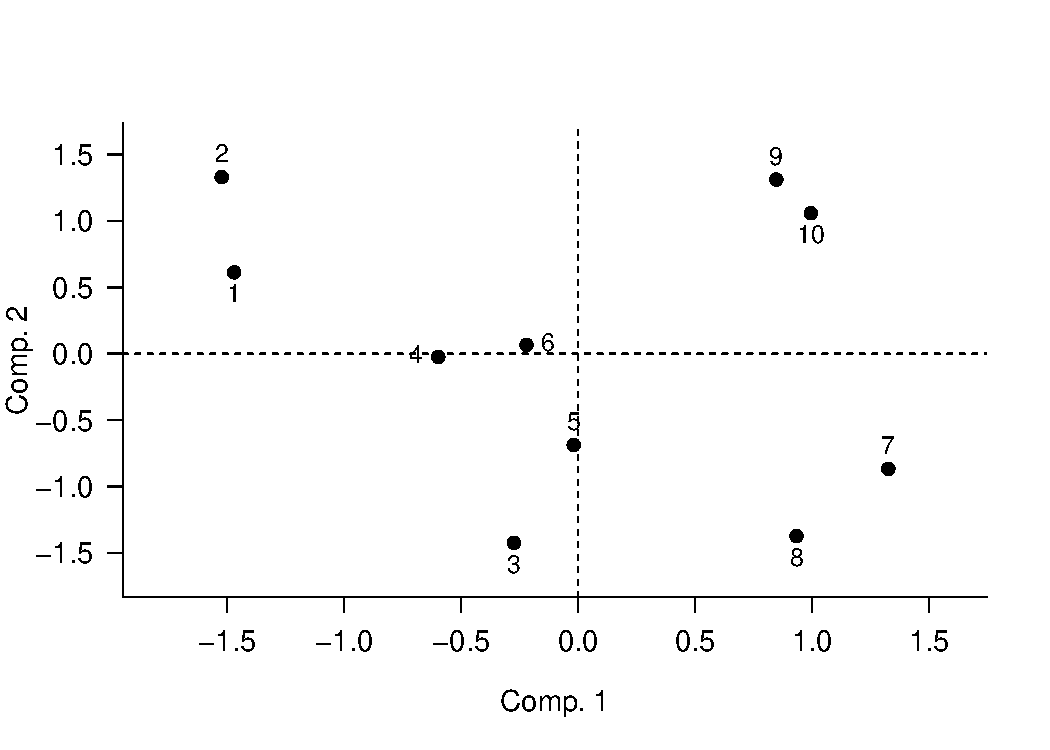
\includegraphics[width=0.65\linewidth]{figura07.pdf}
\caption{Score plot of the two first components in the \textbf{T} matrix}
\label{figura07}
\end{figure}

\begin{figure}[!ht]
\centering
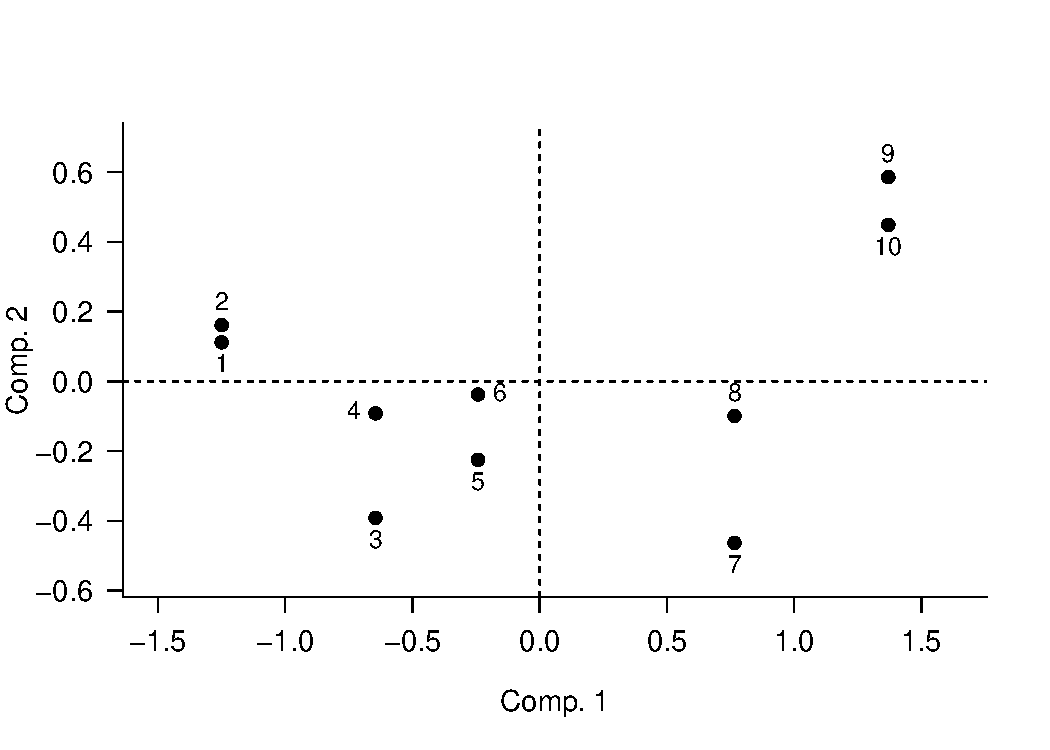
\includegraphics[width=0.65\linewidth]{figura08.pdf}
\caption{Score plot of the two first components in the \textbf{U} matrix}
\label{figura08}
\end{figure}

\autoref{figura07} shows how the 10 samples spread over the two first components. It can be seen how the samples evolve every two observations, from left to right, which seems reasonable attending to their different composition. \autoref{figura08} is similar, but related to the \textbf{y} scores. 

\vspace{15pt}
\begin{lstlisting}[basicstyle=\small, language=Python]
R> plot(fit, type="Wj", cex.axis=1.2, cex.lab=1.2, cex=1.2, 
+    las=1, bty="L")
R> plot(fit, type="Wk", cex.axis=1.2, cex.lab=1.2, cex=1.2, 
+    las=1, bty="L")
\end{lstlisting}

\begin{figure}[!ht]
\centering
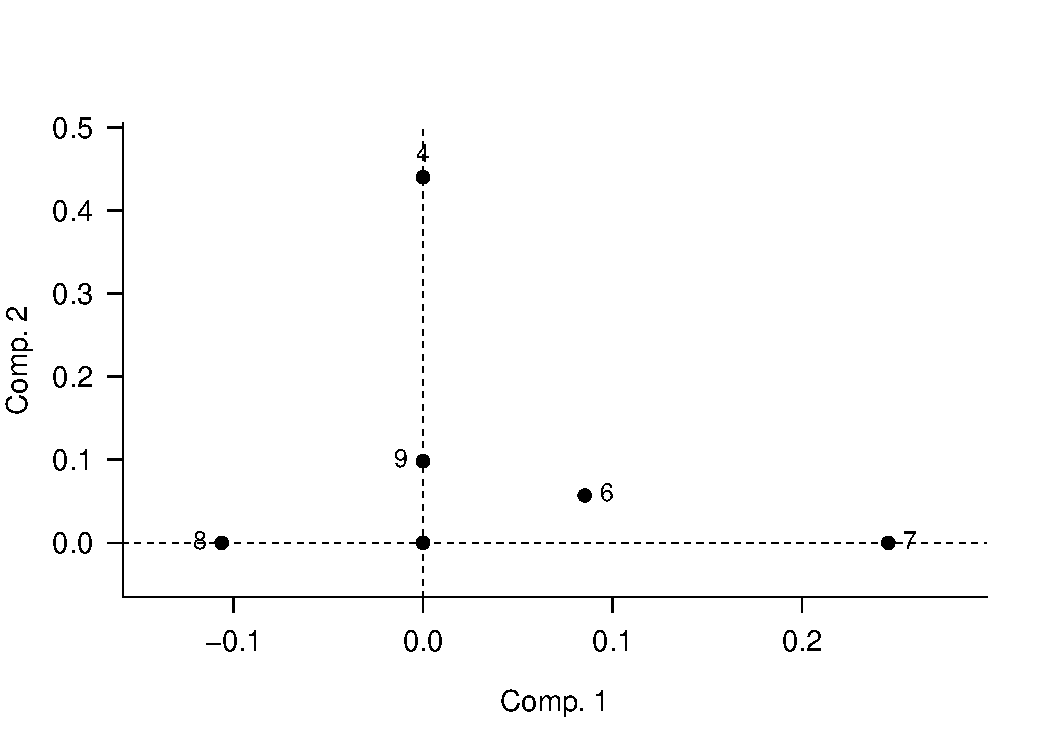
\includegraphics[width=0.65\linewidth]{figura09.pdf}
\caption{Weights Plot of the $\textbf{\text{W}}^{J}$ weights matrix}
\label{figura09}
\end{figure}

On the other hand, \autoref{figura09} presents the attributes and \autoref{figura10} the judges that help in predicting the \textbf{y} variable, for each of the two components. It can be seen that the first component of the attributes mode is related to attributes 7, 8 and 6 (in descending order in absolute values); whereas attributes 4, 9 and 6 are related to the second component. This can be also derived from \autoref{figura11}, which produces an equivalent graph. In this case, when trying to see what kind of relationship these attributes have with the judges’ mode, \autoref{figura12} provides easier-to-interpret results.

\begin{figure}[!ht]
\centering
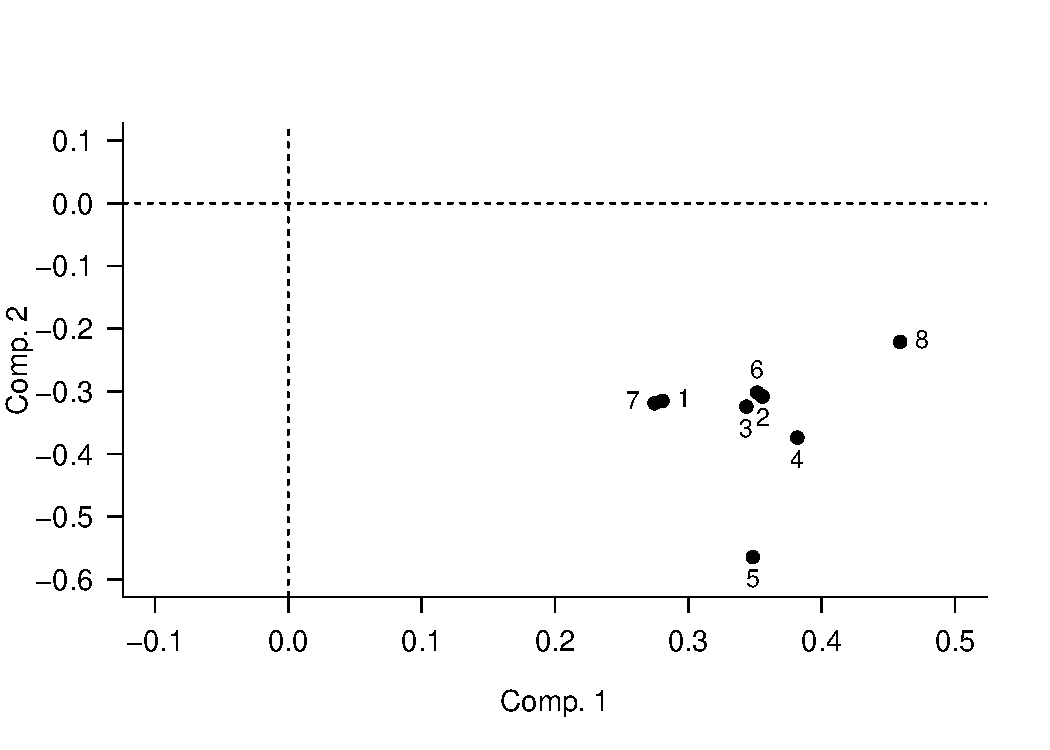
\includegraphics[width=0.65\linewidth]{figura10.pdf}
\caption{Weights Plot of the $\textbf{\text{W}}^{K}$ weights matrix}
\label{figura10}
\end{figure}

\vspace{15pt}
\begin{lstlisting}[basicstyle=\small, language=Python]
R> plot(fit, type="variables", cex.axis=1.2, cex.lab=1.2, 
+   cex=1.2, las=1, bty="L", lwd=2)
R> plot(fit, type="time", cex.axis=1.2, cex.lab=1.2, cex=1.2, 
+   las=1, bty="L", lwd=2, xlab="Judge")
\end{lstlisting}

\begin{figure}[!ht]
	\centering
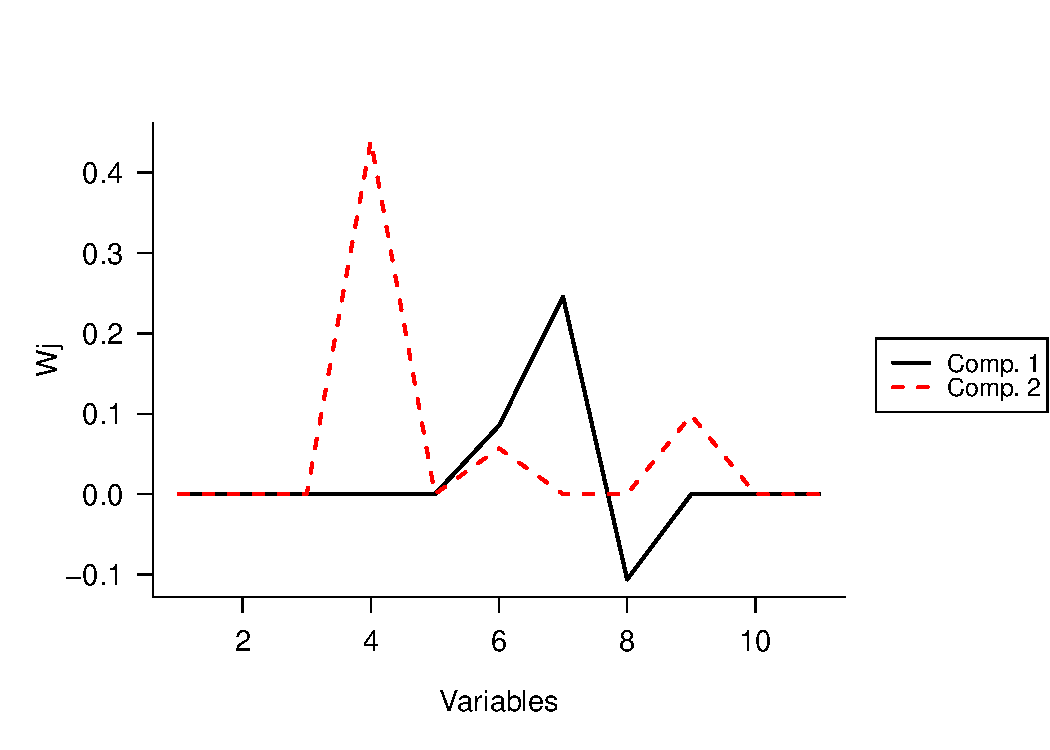
\includegraphics[width=0.65\textwidth]{figura11.pdf}
\caption{Plot of the second mode}
\label{figura11}
\end{figure}

It can be seen how, for the first component, there is approximately the same effect of all judges with respect to variables 7, 8 and 6 (those related to the first component in the attributes mode) when trying to predict the salt content. In this case, since the judges’ weights show positive values, the higher the value of attributes 7 and 6, and the lower the value of attribute 8, the higher the salt content. For the second component, attributes 4, 9 and 6 are more influenced by judge 5, even though the rest of judges also have a similar effect on the salt content scoring (y variable). Since the weights of the judges’ mode are all negative for the second component, the higher the value of attributes 4, 9 and 6, the lower the salt content. In this case, \autoref{figura10} is less interpretable. However, depending on the case, one representation or another might provide easier-to-interpret results; so it is decided to keep both graphs in the package.

\begin{figure}[!ht]
	\centering
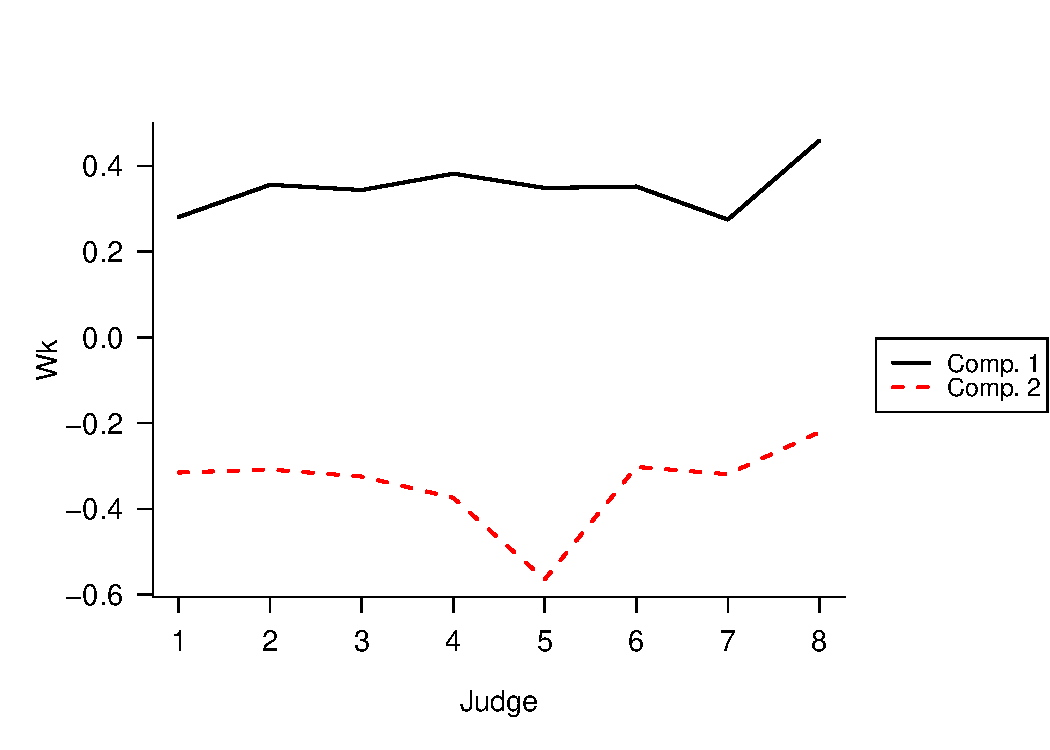
\includegraphics[width=0.7\textwidth]{figura12.pdf}
\caption{Plot of the third mode}
\label{figura12}
\end{figure}
\vspace{10pt}

As seen on these examples, all plots produced by the \texttt{plot.sNPLS} function are fully customizable, being able to change the titles, labels, orientation of labels, axis, size of the plot, etc., by using \textit{base} plot parameters such as \texttt{las}, \texttt{cex}, \texttt{bty}, etc. Since they are base \texttt{R} plots, they can be affected by all \texttt{par} options and also be combined in a single figure by using the \texttt{mfrow} and \texttt{mfcol} options or the \texttt{layout} function.

Finally, the \texttt{predict} function can be used to make predictions using new \textbf{\underline{X}} data. As explained before, it makes use of the coefficients matrix \textbf{B} computed by the \texttt{Rmatrix} function (\autoref{rmatrixf}). Here it is used to make a prediction from a new random \textbf{\underline{X}} array with 10 new observations (\autoref{output5}). This function also has an optional parameter, \texttt{scale}, which defaults to \texttt{TRUE} for controlling the final scale of the predictions (original scale vs. post-processing scale).

\vspace{15pt}
\begin{lstlisting}[basicstyle=\small, language=Python, morekeywords={array, sample, predict}]
newX <- array(sample(0:5, 10*11*8, replace = TRUE), 
+    dim = c(10, 11, 8))
predict(fit, newX)
\end{lstlisting}
\vspace{15pt}
\begin{lstlisting}[basicstyle=\small, backgroundcolor=\color{output}, numbers=none, label={output5}, language=Python, caption=Predictions of the model on new data \texttt{newX}.]
            Y.1
 [1,] 1.4196482
 [2,] 0.7819288
 [3,] 0.9619593
 [4,] 1.0523621
 [5,] 1.2585099
 [6,] 0.7243910
 [7,] 0.6458718
 [8,] 1.2693292
 [9,] 0.8194011
 [10,] 1.2753320
\end{lstlisting}

The output of the function is a \textbf{Y} matrix with the 10 predicted values.

\subsection{Performance}
The package offers a complete set of functions for tuning, fitting and interpreting $N$-PLS and sNPLS models. As tuning is a computationally intensive method, all cross-validation functions in the package allow the use of parallelization through the \textit{parallel} package and also use sparse matrices from the \textit{Matrix} package. This two optimizations allow for speedups of up to 20 times faster computation times compared to non-parallelized computations with dense matrices. The use of sparse matrices also alleviates the use of RAM memory which, in the case of large data sets, could be a limiting factor in some computers. \autoref{figura03} shows the improvements in computing times by using parallelization with different number of cores. As seen in the figure, the multicore scaling allows for tuning a model with a search grid length of 900 in an eight-core machine in less time than it takes to tune a model with a search grid of 90 in a single core running at the same speed.

\begin{figure}[hbtp]
	\centering
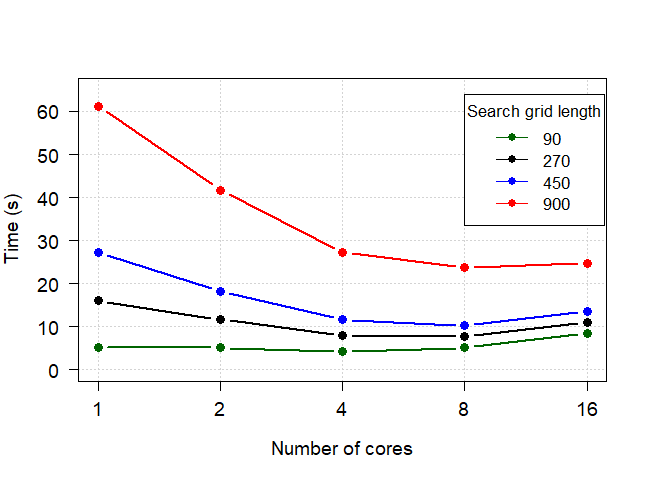
\includegraphics[width=0.65\textwidth]{figura03}
\caption[Computing times of \texttt{cv\_snpls} under different conditions of grid length and number of cores]{Computing times of \texttt{cv\_snpls} under different conditions of grid length and number of cores. The function scales efficiently up until 8 cores}
\label{figura03}
\end{figure}

The package also greatly benefits from the use of specialized Basic Linear Algebra Subprograms (BLAS) such as OpenBLAS, ATLAS or Intel\textsuperscript{\tiny\textregistered}  MKL, which can produce additional speedups of up to 10 times faster computation times \parencite{xianyi2014openblas, wang2014intel}. In this case, the potential benefit is left to the decision of the end user, that should install and link one of these BLAS libraries to \texttt{R}.



% ---------------------------------------------------------------------
% ---------------------------------------------------------------------
% ---------------------------------------------------------------------

\chapter[Validation of the sparse N-PLS method and sNPLS package]{Validation of the sparse N-PLS method and sNPLS package}



% ---------------------------------------------------------------------
% ---------------------------------------------------------------------
\section{Random synthetic data sets}
Our implementation of the L1 penalized $N$-PLS was first tested using data simulation. In total, fourteen different scenarios with different signal-to-noise ratios were tested. Tuning of the models was performed by 20 repetitions of 10-fold cross-validation following the methodology presented in \autoref{chapter:package}. Our simulations consisted on three-way \textbf{\underline{X}} arrays with $I$=50 samples, $J$=50 variables and $K$=3 times, where variables were simulated randomly from different kinds of distributions (Poisson, Normal and Uniform) with varying parameters as follows:

\begin{enumerate}
    \item If Normal: $\mathcal{X}\ {\raise.17ex\hbox{$\scriptstyle\sim$}}\ \mathcal{N}(\mu, \sigma)$\ where $\mu\ {\raise.17ex\hbox{$\scriptstyle\sim$}}\ \mathcal{N}(10, 10)$\ and $\sigma\ {\raise.17ex\hbox{$\scriptstyle\sim$}}\ \Gamma(5, 1)$
    \item If Poisson: $\mathcal{X}\ {\raise.17ex\hbox{$\scriptstyle\sim$}}\ \mathcal{P}(\lambda)$\ where $\lambda\ {\raise.17ex\hbox{$\scriptstyle\sim$}}\ \mathcal{N}(10, 2.5)$
    \item If Uniform: $\mathcal{X}\ {\raise.17ex\hbox{$\scriptstyle\sim$}}\ \mathcal{U}(a, b)$\ where $a\ {\raise.17ex\hbox{$\scriptstyle\sim$}}\ \mathcal{N}(10, 10)$\ and $b\ {\raise.17ex\hbox{$\scriptstyle\sim$}}\ \mathcal{N}(100, 10)$
\end{enumerate}

Only 5 out of the 50 variables were used to construct the response \textbf{\underline{Y}}. They were chosen randomly from the \textbf{\underline{X}} array and assigned randomly the following coefficients: 0.4, 0.5, 0.6, 0.7 and 0.9. In the first run, only one of the three times of the third mode was involved in the creation of, in this case, vector \textbf{y}. In the second run, the three times were involved, but with different coefficients for each variable. In all simulations, random Normal and Poisson errors were added in different amounts to \textbf{y}. For each combination of type and amount of random error, simulations were repeated 100 times. Ability to select the real variables involved in y generation as well as median and 1\textsuperscript{st} and 3\textsuperscript{rd} quartiles of the mean squared error are provided for each simulation run.

Results of the different simulations carried out on the synthetic datasets are provided in \autoref{table:results_synthetic}. Sparse $N$-PLS outperforms $N$-PLS regarding mean squared prediction error. When performing sparse $N$-PLS, the true variables were almost always included in the selected model. Median number of true variables selected in each model was 5 (100\%) in most of the simulations (9 out of 14). In the other 5 simulations, the median number of true variables selected was 4 (80\%). These simulations were the ones consisting in the more complex and noisy models, with the three times of the third mode affecting \textbf{\underline{Y}} and lower signal-to-noise ratios. Also, a varying amount of other noise variables were erroneously included in the models. The amount of noise variables that were included in the sparse $N$-PLS models increased as the signal-to-noise ratio of the data decreased, ranging from a median of 2 (4.4\%) to a median of 7 (15.6\%) noise variables included in the worst-case simulation.

\begin{table}[h!]
\begin{tabular}{ |c|c|c|c| } 
\hline
col1 & col2 & col3 \\
\hline
\multirow{3}{4em}{Multiple row} & cell2 & cell3 \\ 
& cell5 & cell6 \\ 
& cell8 & cell9 \\ 
\hline
\end{tabular}
\caption{Results of the analyses performed using N-PLS and sparse N-PLS on the different simulations. Median (1\textsuperscript{st}, 3\textsuperscript{rd} quartile) of the mean squared error and a 95\% confidence interval for the difference in mean squared error between sparse $N$-PLS and $N$-PLS is also provided. True variables selected column indicates the median of the occasions these are included in the models, as well as the 1\textsuperscript{st} and 3\textsuperscript{rd} quartiles (True positives). Noise variables selected column presents analogous results for the Noise variables (False positives)}
\label{table:results_synthetic}
\end{table}

\section{Data driven synthetic data sets}
To further test the performance of the method in selecting highly correlated variables, simulated data resembling the ones of a  toxicogenomics data set \parencite{heijne2004bromobenzene} was analysed. In this work, the effect of the hepatotoxicant bromobenzene in rats was studied. Groups of rats were treated with different doses of this toxic compound dissolved in corn oil for a 48 hours period. At three time points from the start of the treatment, rats were sacrificed. Liver samples were used to extract mRNA for microarray profiling and blood and urine was used for metabolite profiling. Additionally, 21 physiological parameters were recorded: Glucose, A/G ratio, GSH, Body Weight, Creatin, GGT, Urea, Kidneys, Kidney/BW, Triglycerides, Liver, Albumin, Total Protein, ALP, Liver/BW, Bilirubin, LDH, Phospholipids, Cholesterol, ASAT, ALAT. 

In this work, simulated profiles from 14 of these 21 physiological parameters were used to discriminate between two of the different groups (High and Low doses evolution). In order to compute these profiles, since they were not shown in \parencite{heijne2004bromobenzene}, we took advantage of those shown in \cite{conesa2010multiway}, which correspond to the same dataset. 25 samples for high doses and 25 for low doses were simulated, adding to the pattern random normal noise, with standard deviation 0.1.

\autoref{figura29} represents time course levels of the seven patterns corresponding to the 14 physiological parameters evaluated for high and low dose treatment groups. 

\begin{figure}[hbtp]
	\centering
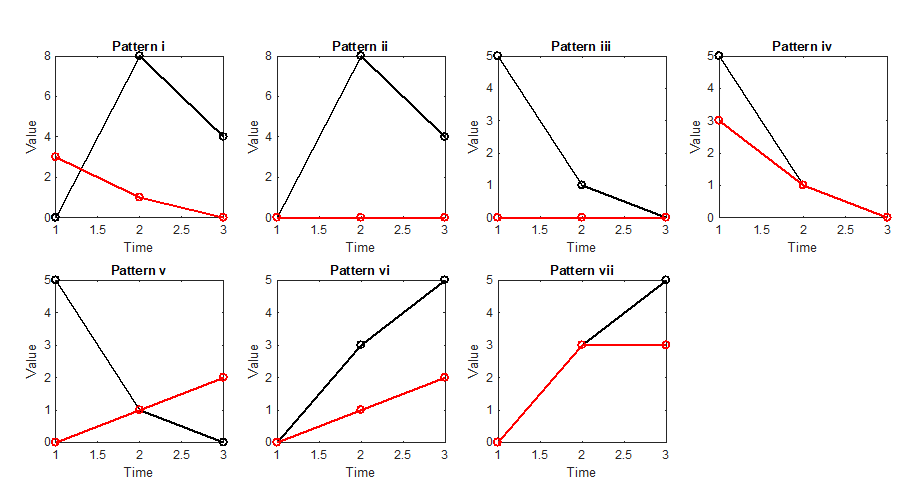
\includegraphics[width=0.7\textwidth]{figura29.png}
\caption{Patterns for the 14 different variables in both groups: High doses (red lines) and low doses (black lines).}
\label{figura29}
\end{figure}

These variable can be grouped attending to their common patterns in the following groups; i) ALT, AST, LDH and GSH; ii) Creatin and Albumin; iii) Kidney and Cholesterol; iv) Liver, Phospholipids and Triglycerides; v) Glucose; vi) A/G Ratio and vii) Urea.

In this case, the goal was to test the ability of the sparse N-PLS model for gathering those relevant variables within the Lasso selection procedure even in the case that these variables show correlation. \autoref{table:results_synth2} summarizes the model coefficients obtained in the data set analysis.. Overall, results of the analysis showed good agreement with the structure of the data. All the variables  following the pattern i (i.e., ALT, AST, LDH and GSH) were selected by the method and similar coefficients  were assigned Additionally, Creatinine and Albumin (pattern ii) were also selected with similar coefficients. Interestingly,  the A/G ratio (pattern vi), a variable uncorrelated to all the others was also selected. However, kidney and cholesterol were not selected by the model, probably because selection was also performed on the third mode and only the third element of the third mode was selected (\autoref{table:results_synth2}).

\begin{table}[!h]
\begin{tabular}{ |c|c|c|c| } 
 \hline
 \  & T1 & T2 & T3 \\ 
 Glucose & 0 & 0 & 0 \\ 
 Phospholipids & 0 & 0 & 0 \\ 
 Kidney & 0 & 0 & 0 \\ 
 Cholesterol & 0 & 0 & 0 \\ 
 Tryglycerids & 0 & 0 & 0 \\ 
 A/G ratio & 0 & 0 & 0.077 \\ 
 Urea & 0 & 0 & 0 \\ 
 Creatinine & 0 & 0 & 0.082 \\ 
 Albumin & 0 & 0 & 0.076 \\ 
 ALT & 0 & 0 & 0.221 \\ 
 AST & 0 & 0 & 0.221 \\ 
 LDH & 0 & 0 & 0.221 \\ 
 GSH & 0 & 0 & 0.101 \\ 
 \hline
\end{tabular}
\caption{Coefficients of the model}
\label{table:results_synth2}
\end{table}

\section{Real data sets}
Liquid chromatography–mass spectrometry (LC-MS) analyses of rat serum samples were performed in an Agilent 1290 Infinity LC system coupled to an Agilent 6550 Q-TOF mass spectrometer equipped with an ESI source (Agilent Technologies, Santa Clara, CA, USA). LC-MS grade solvents (i.e. water, acetonitrile and methanol) were acquired from Fisher Scientific (Loughborough, UK). All the LC-MS additives and standards were acquired from Sigma–Aldrich/Fluka (Madrid, Spain). Metabolites were separated on an Zorbax SB-Aq column (100 x 2.1 mm; 1.8 {\textmu}m (Agilent Technologies, Santa Clara, CA, USA). Mobile phases consisted of (A) 1mM ammonium fluoride and (B) acetonitrile. The separation was conducted under the following gradient at a flow of 0.3 mL/min: 0 min 3 \% (B); 0–2 min 40 \% (B); 2-5 min 7 \% (B); 5-7 min 50 \% (B); 7-12 min 100\% (B); 12-16min 100\% (B); 16-16.5 min 3\% (B); 16.5-18 min 3\% (B). Sample and column temperatures were maintained at 4 ºC and 40ºC, respectively. The injection volume was 5 {\textmu}L. 
The instrument was tuned in the 50-1700 m/z range using an Agilent tune mix in 2GHz extended dynamic range mode (mass resolving power 25,000 FWHM). Detection was performed in ESI (-) mode in the 50-1000 m/z range. A reference solution (m/z 119.0360 and m/z 980.0164) was used to correct small mass drifts during acquisition. The following conditions were employed: capillary voltage, 3.5 kV; nozzle voltage -1.0 kV; fragmentor voltage, 175 V; gas temperature, 200 ºC; drying gas (nitrogen), 14 L/min; nebulizer gas (nitrogen), 35 psi; sheath gas temperature, 350 ºC; and sheath gas flow (nitrogen), 11 L/min. The acquisition rate was set at 4 spectra/s in all cases. Data preprocessing was performed using ProgenesisQI software (Nonlinear Dynamics, UK).

Six-week-old male Oncins France Strain A (OFA) rats (200–240 g) were purchased from Charles River (Barcelona, Spain) and acclimatized to laboratory conditions for at least 7 days. Animals were housed (12-h light-dark cycle, 21–25°C, 30–70\% humidity, woodchip bedding) and fed ad libitum with a standard chow diet (Scientific Animal Food and Engineering, Augy, France). Rats were anesthetized with sodium thiobarbital (0.1 g/kg), and blood was collected by cardiac puncture. After coagulation and centrifugation (1,000 g for 10 min at 4°C), serum samples were aliquoted and stored at - 80°C until the analysis. All the experimental protocols were approved by the Institutional Animal Ethics Committee. 40 {\textmu}L of serum sample were mixed with 120 µL of methanol. After vortexing, samples were kept at -20 ºC for 20 min. Samples were centrifuged (14000 g, 4 ºC, 15 min) and the supernatants transferred to clean tubes and evaporated to dryness. Samples were resuspended in 80 {\textmu}L of water, centrifuged (14000 g, 4 ºC, 5 min), and the clean supernatants transferred to HPLC vials for their LC-MS analysis. Rats serum samples were separated in two groups of sizes 8 and 6 and subsequently fortified with a set of metabolites to generate the patterns showed in \autoref{figura30}. Metabolites and final concentrations used are summarized in \autoref{table:metabolites}.

\begin{figure}[hbtp]
	\centering
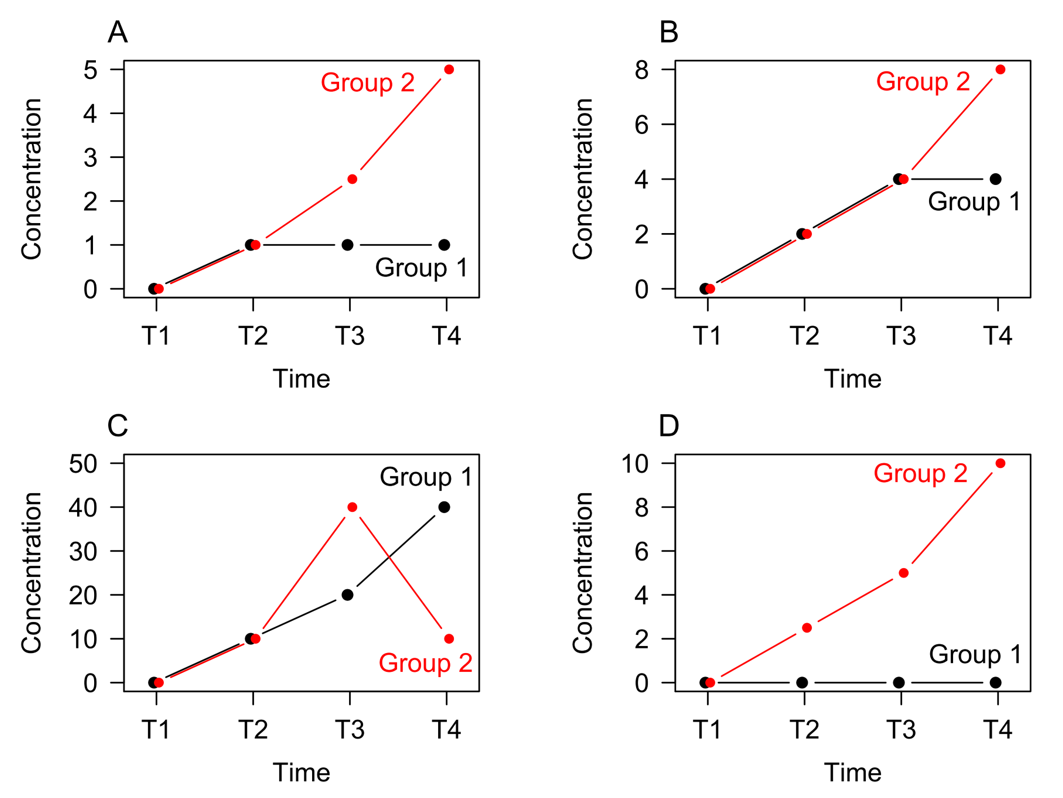
\includegraphics[width=0.7\textwidth]{figura30.png}
\caption{Expected patterns for the four different metabolite classes in group 1 (n=8) and group 2 (n=6).}
\label{figura30}
\end{figure}

\begin{table}[h!]
\begin{tabular}{ |c|c|c|c| } 
\hline
col1 & col2 & col3 \\
\hline
\multirow{3}{4em}{Multiple row} & cell2 & cell3 \\ 
& cell5 & cell6 \\ 
& cell8 & cell9 \\ 
\hline
\end{tabular}
\caption{List of metabolites for each variable class. Metabolites are grouped attending to their physical and chemical properties. Class A, comprises fatty acid; Class B, comprises bile acids; Class C, comprises amino acids; Class D comprises miscellaneous compounds}
\label{table:metabolites}
\end{table}

Simulated data sets provide a useful suitable first approach to test the performance of the new sNPLS method. However, to exemplify sNPLS its utility in a more complex context, the proposed method was faced to the analysis a real a real dataset, which was derived from a metabolomics study. In the metabolomics data sets usually hundreds of variables, with high noise and high correlation are obtained, which dramatically hinders biomarker discovery and variable selection for predictive models building.  Thus, real processed rat serum samples were used to artificially generate two different groups by adding a set of standards at different final concentrations that additionally  showed different trends along time (\autoref{figura30}).  In our opinion, this experimental design provides a suitable frame work to assess sNPLS capabilities when facing real -omics data sets.
Our cross-validation procedure (20 repetitions of 5-fold cross-validation) selected as the optimum parameter values 30 features of \textbf{W}\textsuperscript{J}, 3 features of \textbf{W}\textsuperscript{K} and 2 components. Therefore, 60 variables among the initial 1220 obtained from the LC-MS analysis (30 in each component) were selected by our final sparse $N$-PLS model. Out of the four variable classes which were different between both groups by design (\autoref{table:metabolites}), our model included at least one representative variable for each class. The model also included other variables not present among the four controlled variable classes, but many of them showed similar patterns to those included and could be derivatives or adducts of the original metabolites. Overall, the selection provided by the new model showed a quite feasible result, where not only the real assignable variables (added metabolites) but also those interfering ones can be selected. A list of all the selected variables is presented in \autoref{table:results_real}. The first column list those variables selected by sparse $N$-PLS, while  the second column indicates on which component these variables were selected. The third column shows wether these variables belong or not to one of the classes described in \autoref{table:metabolites}. Finally, column four shows whether those variables that do not belong to any of the assayed classes follows or not a pattern similar to those variables included (Table 1). Interestingly, variables of the classes 1, 2 and 3 and its derivatives or analogues were all exclusively selected in the first component and variables of the class 4 and its derivatives or analogues were all exclusively selected in the second component. Variables with different patterns to those of the four experimentally generated classes were included in both components, but were more prominent in the second one (13 in the first component versus 20 in the second). 

Finally, the performance of our model was compared with the standard $N$-PLS model. To this end, the metabolomics data set was analysis using both approaches. The sNPLS model clearly discriminated between the two rat groups (\autoref{figura31}A). However, similar groups’ separation was also obtained by suing the standard $N$-PLS (\autoref{figura31}B). The differences between both models appear when comparing \autoref{figura31}B vs \autoref{figura31}G, and \autoref{figura31}C vs \autoref{figura31}H, related to \textbf{W}\textsuperscript{J} and \textbf{W}\textsuperscript{K}, respectively; or \autoref{figura31}D vs \autoref{figura31}I, and \autoref{figura31}E vs \autoref{figura31}J respectively, which are alternative representations. For interpretation purposes, it seems better to compare \autoref{figura31}B vs \autoref{figura31}G for \textbf{W}\textsuperscript{J}, and \autoref{figura31}E vs \autoref{figura31}J for \textbf{W}\textsuperscript{K}. For \textbf{W}\textsuperscript{J}, it seems quite clear that the selection made from sparse $N$-PLS allows a clear interpretation of the metabolites responsible for the separation between the two groups. In the first component, are represented those metabolites belonging to the classes 1, 2 and 3. While, the second component is related to completely independent metabolites (with respect to component one), which could be related to the separation of rats 6 and 13. Many of these metabolites are from class 4, although some of them are not apparently related to any of the designed variable groups.
These interpretations are much more hard to do when using standard $N$-PLS due to the high number of variables to deal with in the second (metabolites) mode, so from this perspective the proposed approach seems to improve the standard $N$-PLS model when trying to directly select the variables of interest (metabolites in this case). However, it should be highlighted that variable selection is out of the $N$-PLS scope. These results shows that when variable selection is of prior relevance for interpretation or validation purposes sparse $N$-PLS come up as a valid alternative
For the interpretation of \textbf{W}\textsuperscript{K}, \autoref{figura31}E and \autoref{figura31}J have been selected. These plots show,  for the first component, a similar pattern, although a slight shift downwards is observed for the standard $N$-PLS. The similar trend observed for both methods strengths the use of the sparse $N$-PLS results, as it provides extra information as discussed above. However, regarding the second component, they do not provided the same result, which could be related to the clear separation of rats 6 and 13 observed in sparse $N$-PLS (\autoref{figura31}A).

\begin{figure}[hbtp]
	\centering
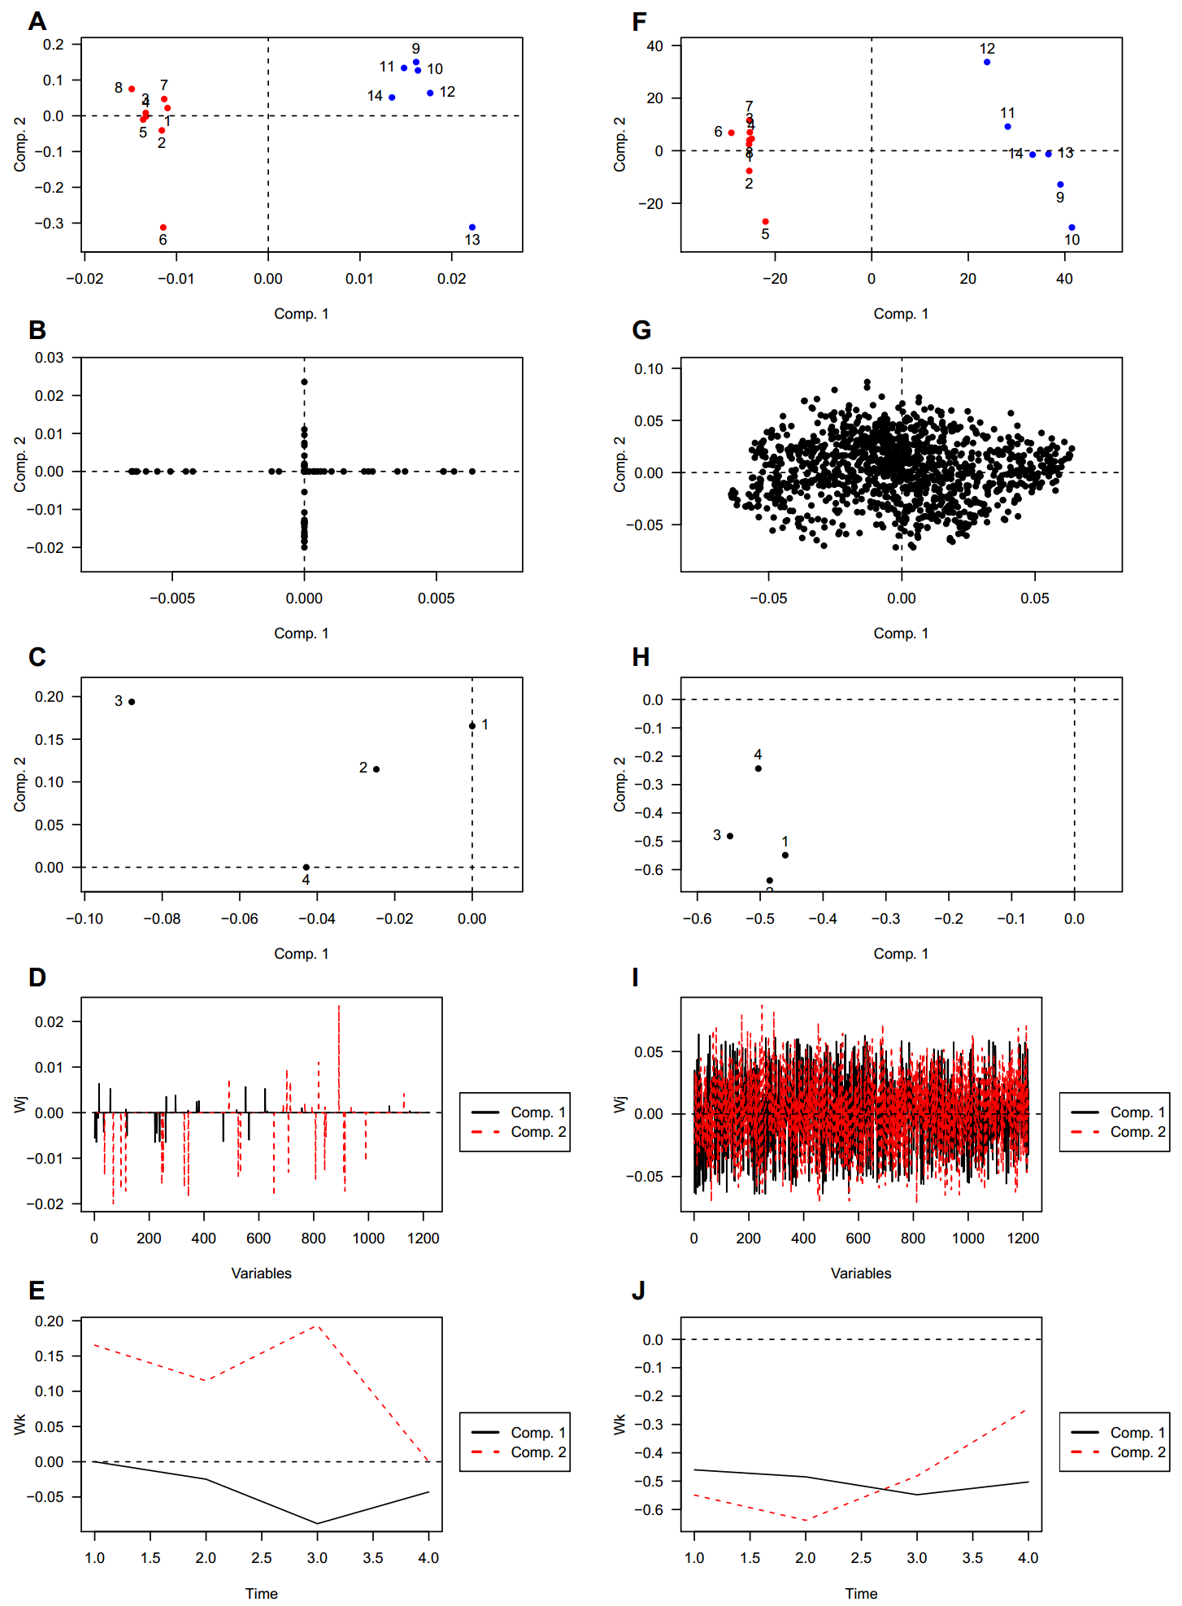
\includegraphics[width=0.95\textwidth]{figura31.png}
\caption{Plots of the sparse $N$-PLS model (left) and the standard $N$-PLS model (right). Score plots of the two first components in the \textbf{T} matrix (A, F); weighting plots of the \textbf{W}\textsuperscript{J} matrix (B, G); weighting plot of the \textbf{W}\textsuperscript{K} matrix (C, H); plots of the loadings of the second (D, I) and third (E, J) modes.}
\label{figura31}
\end{figure}

\section{Comparison with other methods}

% ---------------------------------------------------------------------
% ---------------------------------------------------------------------
% ---------------------------------------------------------------------
\part{Conclussions, discussion and future work}
\chapter[Conclusions]{Conclusions and future work}

% ---------------------------------------------------------------------
% ---------------------------------------------------------------------
\section{Developed topics and contributions}
This thesis has covered the issues and difficulties in analyzing metabolomic data and the different techniques able to deal with those problems. A special focus has been given to the treatment and analysis of three-way and, by extension, multi-way data sets and the development and implementation of a variable selection procedure integrated at the model-fitting step.

First, a review of the properties and particularities of 'omic' data and, more specifically, of metabolomic data was performed. The main characteristics of these data are their multicollinearity, the large number of variables and their organization in complex data structures. There are a wide range of methods available for analyzing metabolomic data sets. In this thesis, many of these techniques have been presented and explained; after a review of the classical statistical methods, such as univariate tests, were their limitations have been exposed, we have assessed the usefulness of PCA, PLS, ridge regression, lasso, elastic net, random forest and boosting for the analysis of metabolomic data. After this, we have focused on complex data structures such as three-way or multi-way arrays and the tools for their analysis regarding compression methods such as Tucker3 and PARAFAC and also predictive modelling methods such as $N$-PLS.

A new method for combining the $N$-PLS algorithm with L1-penalization has been developed. This method is applied at the determination of the $\textbf{\text{w}}^J$ and $\textbf{\text{w}}^K$ to achieve sparse versions of the latent variables and effectively perform variable selection at the model fitting step. The penalization of both vectors, $\textbf{\text{w}}^J$ and $\textbf{\text{w}}^K$, achieves not only variable selection on the second mode ($J$), but also on the third mode ($K$). Related to the variable selection, this method allows for the construction of simpler models than standard $N$-PLS. This makes the models more interpretable and less prone to overfitting.

The new developed method sNPLS has been implemented in an R package called \texttt{sNPLS}. This package includes not only the main sNPLS algorithm but also a complete set of functions for fitting predictive models with three-way data structures, including parallelized cross-validation and repeated cross-validation procedures, processing of the data such as centering, scaling and unfolding and a wide array of plots for interpretation of the modelling results. Additionally, this is the only package for performing $N$-PLS regression models in \texttt{R}, so with its development we have expanded the applicability of three-way methods to the \texttt{R} user community.

The method and its implementation in \texttt{R} has also been validated using synthetic simulations and real data sets, showing lower prediction error than standard $N$-PLS and good performance in variable selection. The method has also been validated for the case of high multicollinearity between variables, proving that the combination of L1-penalization and $N$-PLS projection behaves similarly to elastic net, being able to select all correlated variables instead of discarding most of them and selecting only one as happens with lasso. 

Additionally, we have compared the variable selection performance of sNPLS to other methods such as VIP scores and SR, obtaining similar results with the three methods, with any of them being superior to the other two in some cases and inferior in other cases.

\section{Future work and research lines}
The development of a new method for performing variable selection at the model-fitting step in $N$-PLS and its software implementation as an \texttt{R} package has opened a large range of research lines that should be explored in the future. These research lines can be framed in three different categories: methodological developments, software development and practical application of the method to real problems in biomedical research.

Regarding methodological developments, future research lines include:

\begin{enumerate}
    \item Study of other possible penalizations such as L0 or adaptive L1 penalization. The field of penalized regression methods is a very active research branch. Since our method is a combination of a projection based method with a penalization method, advances both fields could be incorporated into our technique. Adaptive L1 penalization is specially appealing for its oracle properties \parencite{zou2006adaptive}.
    \item Development of alternative methods for the selection and/or tuning of the hyperparameter space. Using $RMSE$ for the tuning of the hyperparameters results in a theoretically optimal prediction error performance at a cost of non-optimal variable selection performance. Finding an appropriate criterion for achieving optimal variable selection performance would greatly increase the flexibility and utility of the method.
    \item Derivation of standard errors and confidence intervals for sNPLS to further improve the inference capabilities of the method.
\end{enumerate}
\vspace{10pt}
In the case of software development, the proposed future research lines include:

\begin{enumerate}
    \item Improvement of the \texttt{sNPLS} \texttt{R} package as exposed in \autoref{packagedev}. This includes adding all the functionality developed by the methodological research lines, but also improving the efficiency of the computations and adding more data processing options and plots.
    \item Developing an alternative to the search grid method. Random search is one candidate, but other options should be studied such as gradient search or genetic algorithms.
    \item Study the impact of the use of different BLAS libraries on the performance of the package and implement optimizations in the algorithm based on this results.
\end{enumerate}
\vspace{10pt}
Finally, regarding practical application of the method to real biomedical problems, the potential number of research lines is immense, so a generic sample is provided:

\begin{enumerate}
    \item Application of the sNPLS method to biomarkers search in longitudinal studies.
    \item Development of prediction models for outcome in repeated measures studies.
    \item Use of the sNPLS method for the understanding of complex biological systems
\end{enumerate}


% -------------------------------------------------------
% -------------------------------------------------------
% -------------------------------------------------------
% Bibliografía

\bibitemsep = 3ex
\bibhang = 2em

\printbibliography[heading=bibintoc,title=\bibname]

% -------------------------------------------------------
% Índice alfabético

\cleardoublepage
\phantomsection
\addcontentsline{toc}{chapter}{\indexname}

\printindex

% -------------------------------------------------------
% Fin del documento

\end{document}

% ---------------------------------------------------------------------
% ---------------------------------------------------------------------
% ---------------------------------------------------------------------
